\documentclass[10pt, a4paper]{article}
\usepackage[slovene]{babel}
\usepackage[T1]{fontenc}
\usepackage[utf8]{inputenc}
\usepackage{lmodern}
\usepackage{amsmath}
\usepackage{amsthm}
\usepackage{amssymb}
\usepackage{parskip}
\usepackage{pgfplots}
\pgfplotsset{compat=1.16}
\usepgfplotslibrary{colormaps,fillbetween}
\usepackage{comment}
\usepackage{graphicx}
\usepackage{booktabs}
\usepackage{array}
%\usepackage{mdframed}
%\usepackage{thmbox}

%%%%%%%%%%%%%%%%%%%%%%%%%%%%%%%%%%%%%%%%%%%%%%%%%%%%%%%%%%%%%%%%%%%%%%

\usepackage[top=105pt, bottom=75pt, left=75pt, right=75pt]{geometry}
\setlength{\headsep}{15pt}
\setlength{\footskip}{45pt}

\usepackage{xcolor}
\usepackage{lipsum}

\usepackage{ifthen}
\usepackage{tikz}
\usetikzlibrary{calc}



%%%%%%%%%%%%%%%%%%%%%%%%%%%%%%%%%%%%%%%%%%%%%%%%%%%%%%%%%%%%%
\usepackage{tcolorbox}
\tcbuselibrary{skins, breakable}


%%%%%%%%%%%%%%%%%%%%%%%%%%%%%%
%%% with separate title
\xdefinecolor{thmTopColor}{RGB}{102, 102, 238}
\xdefinecolor{thmBackColor}{RGB}{245, 245, 255}

%%%%%%%%%%%%%%%%%%%%%%%%%%%%%%%%%%%%%%%%%%%%%%%%%%%%%%%%%%%%%%%%%%%%%%%%

\graphicspath{ {./images/} }

\newtheorem{izr}{Izrek}[section]

\newenvironment{thmbox}[1]{%
  \tcolorbox[%
  empty,
  parbox=false,
  noparskip,
  enhanced,
  breakable,
  sharp corners,
  boxrule=-1pt,
  left=2ex,
  right=0ex,
  top=0ex,
  boxsep=1ex,
  before skip=2.5ex plus 2pt,
  after skip=2.5ex plus 2pt,
  colback=thmBackColor,
  colframe=white,
  coltitle=black,
  colbacktitle=thmBackColor,
  fonttitle=\bfseries,
  title=#1,
  titlerule=1pt,
  titlerule style=thmTopColor,
  overlay unbroken and last={%
    \draw[color=thmTopColor, line width=1.25pt]
    ($(frame.north west)+(.5em, -4.1ex)$)
    -- ($(frame.south west)+(.5em, 1ex)$) -- ++(2em, 0);
  }]
}{\endtcolorbox}

\newenvironment{izrek}[1][]{% before
  \refstepcounter{izr}%
  \ifthenelse{\equal{#1}{}}{%
    \begin{thmbox}{Izrek \theizr.}\itshape\hspace{-.75ex}%
  }{%
    \begin{thmbox}{Izrek \theizr%
        \hspace{.75ex}(\textnormal{#1}).}\itshape\hspace{-.75ex}
    }}
  {\end{thmbox}
}

{\theoremstyle{plain}
\newtheorem{posledica}[izr]{Posledica}
\newtheorem{trditev}[izr]{Trditev}

}

{\theoremstyle{definition}
\newtheorem{defi}{Definicija}[section]
\newtheorem{aksiom}{Aksiom}[section]
}

\newenvironment{noticeB}{%
  \tcolorbox[%
  notitle,
  empty,
  enhanced,  % delete the edge of the bottom page for a broken box
  breakable,
  coltext=black,
  colback=white, 
  fontupper=\rmfamily,
  parbox=false,
  noparskip,
  sharp corners,
  boxrule=-1pt,  % width of the box' edges
  frame hidden,
  left=7pt,  % inner space from text to the left edge
  right=7pt,
  top=5pt,
  bottom=5pt,
  % boxsep=0pt,
  before skip=2.5ex plus 2pt,
  after skip=2.5ex plus 2pt,
  borderline west = {1.5pt}{-0.1pt}{blue!30!black}, % second argument = offset
  overlay unbroken and last={%
    \draw[color=black, line width=1.25pt]
    ($(frame.south west)+(1.pt, -0.1pt)$) -- ++(2em, 0);
  }
  ]}
{\endtcolorbox}

\newenvironment{definicija}{\begin{defi}\begin{noticeB}}{%
    \end{noticeB}\end{defi}}

{\theoremstyle{remark}
\newtheorem*{opomba}{Opomba}
}

\newtheorem{zgled}{Zgled}[section]
\tcolorboxenvironment{zgled}{%
  enhanced jigsaw,
  boxrule=-1pt,
  colframe=gray!15,
  %borderline west={2pt}{0pt}{black},  % second argument is the offset
  interior hidden,
  sharp corners,
  breakable,
  before skip=2.5ex plus 2pt,
  after skip=2.5ex plus 2pt
}

%%%%%%%%%%%%%%%%%%%%%%%%%%%%%%%%%%%%%%%%%%%%%%%%%%%%%%%%%%%%%%%%%%%%%%%%
\newtheorem{lema}[izr]{Lema}
\tcolorboxenvironment{lema}{%
  enhanced jigsaw,
  boxrule=-1pt,
  sharp corners,
  colframe=white,
  borderline west={2pt}{0pt}{orange},  % second argument is the offset
  interior hidden,
  breakable,
  before skip=2.5ex plus 2pt,
  after skip=2.5ex plus 2pt
}

%%%%%%%%%%%%%%%%%%%%%%%%%%%%%%%%%%%%%%%%%%%%%%%%%%%%%%%%%%%%%%%%%%
\newenvironment{noticeC}{%
  \tcolorbox[%
  notitle,
  empty,
  enhanced,  % delete the edge of the bottom page for a broken box
  breakable,
  coltext=black, 
  fontupper=\rmfamily,
  parbox=false,
  noparskip,
  sharp corners,
  boxrule=-1pt,  % width of the box' edges
  frame hidden,
  left=7pt,  % inner space from text to the left edge
  right=7pt,
  top=5pt,
  bottom=5pt,
  % boxsep=0pt,
  before skip=2.5ex plus 2pt,
  after skip=2.5ex plus 2pt,
  %borderline west = {1.5pt}{-0.1pt}{gray}, % second argument = offset
  overlay unbroken and last={%
    %\draw[color=gray, line width=1.25pt]
    %($(frame.west)$);
    %\draw[color=gray, line width=1.25pt]
    %($(frame.east)$);
  },
  ]}
{\endtcolorbox}

\newenvironment{dokaz}%
  {\begin{noticeC}\begin{proof}}%
  {\end{proof}\end{noticeC}}

%%%%%%%%%%%%%%%%%%%%%%%%%%%%%%%%%%%%%%%%%%%%%%%%%%%%%%%%%%%%%%%%%%%%

\makeatletter
\newlength\xvec@height%
\newlength\xvec@depth%
\newlength\xvec@width%
\newcommand{\xvec}[2][]{%
  \ifmmode%
    \settoheight{\xvec@height}{$#2$}%
    \settodepth{\xvec@depth}{$#2$}%
    \settowidth{\xvec@width}{$#2$}%
  \else%
    \settoheight{\xvec@height}{#2}%
    \settodepth{\xvec@depth}{#2}%
    \settowidth{\xvec@width}{#2}%
  \fi%
  \def\xvec@arg{#1}%
  \def\xvec@dd{:}%
  \def\xvec@d{.}%
  \raisebox{.2ex}{\raisebox{\xvec@height}{\rlap{%
    \kern.05em%  (Because left edge of drawing is at .05em)
    \begin{tikzpicture}[scale=1]
    \pgfsetroundcap
    \draw (.05em,0)--(\xvec@width-.05em,0);
    \draw (\xvec@width-.05em,0)--(\xvec@width-.15em, .075em);
    \draw (\xvec@width-.05em,0)--(\xvec@width-.15em,-.075em);
    \ifx\xvec@arg\xvec@d%
      \fill(\xvec@width*.45,.5ex) circle (.5pt);%
    \else\ifx\xvec@arg\xvec@dd%
      \fill(\xvec@width*.30,.5ex) circle (.5pt);%
      \fill(\xvec@width*.65,.5ex) circle (.5pt);%
    \fi\fi%
    \end{tikzpicture}%
  }}}%
  #2%
}
\makeatother

% --- Override \vec with an invocation of \xvec.
\let\stdvec\vec
\renewcommand{\vec}[1]{\xvec[]{#1}}
% --- Define \dvec and \ddvec for dotted and double-dotted vectors.
\newcommand{\dvec}[1]{\xvec[.]{#1}}
\newcommand{\ddvec}[1]{\xvec[:]{#1}}
\newcommand{\stcomp}[1]{{#1}^{\mathsf{c}}}

%%%%%%%%%%%%%%%%%%%%%%%%%%%%%%%%%%%%%%%%%%%%%%%%%%%%%%%%%%%%%%%%%%%%

\newcommand{\N}{\mathbb {N}}
\newcommand{\Z}{\mathbb {Z}}
\newcommand{\Q}{\mathbb {Q}}
\newcommand{\R}{\mathbb {R}}
\newcommand{\C}{\mathbb {C}}
\newcommand{\zap}[1]{(#1_n)_{n=1} ^{\infty}}
\newcommand{\podzap}[1]{(#1_{n_j})_{n=1 ^{\infty}}}
\newcommand{\limzap}[1]{\lim_{n \to \infty} {#1}}
\newcommand{\ve}[1]{\overrightarrow{#1}}
\newcommand{\vectors}[2]{\vec{{#1}_1},\vec{{#1}_2}, \dots \vec{{#1}_{#2}}}
\newcommand{\scalars}[2]{{#1}_1, {#1}_2, \dots, {#1}_{#2}}
\newcommand{\im}{\mathrm{\text{im}}\,}
\newcommand{\rang}{\mathrm{\text{rang}}\,}
\newcommand{\isom}{\stackrel{\sim}{=}}
\newcommand{\quot}[2]{{\raisebox{.2em}{$#1$}\left/\raisebox{-.2em}{$#2$}\right.}}
\newcommand{\sprod}[2]{\left\langle {#1},{#2} \right\rangle}
\newcommand{\cl}{\mathrm{Cl}}
\newcommand{\inte}{\mathrm{Int}}
\newcommand{\fr}{\mathrm{Fr}}
\newcommand{\F}{\mathcal{F}}
\DeclareMathOperator{\di}{d\!}

\newcolumntype{C}[1]{>{\centering\let\newline\\\arraybackslash\hspace\hspace{0pt}}m{#1}}

\setlength{\parskip}{1em}

\begin{document}

\title{ANALIZA 2a - ZAPISKI}
\author{Gal Anton Gorše}
\date{}
\maketitle

\section{FUNKCIJE IN PRESLIKAVE VEČ SPREMENLJIVK}

\subsection{Uvod}

Na množici $\overbrace{\R \times \dots \times \R}^n$ urejenih $n$-teric $(x_1, x_2, \dots, x_n)$
imamo operacijo seštevanja po komponentah in množenje s skalarjem po komponentah. Iz linearne algebre vemo, da 
ti operaciji ustrezata aksiomom vektorskega prostora. Množica $\R^n$ je torej 
$n$-razsežni vektorski prostor in njegovo standardno bazo sestavljajo vektorji $(1, 0, \dots, 0),\ (0, 1, \dots, 0), \dots, (0, 0, \dots, 1)$.

Na tem prostoru imamo definiran standardni skalarni produkt. Ta je za vektorja $x=(x_1, \dots, x_n)$
in $y = (y_1, \dots, y_n)$ podan s predpisom $\sprod{x}{y} = x_1 y_1 + \dots + x_n y_n$.
Ta skalarni produkt nam inducira normo $|x| = \sqrt{x \cdot x} = \sqrt{x_1 ^2 + \dots + x_n^2}$.
Slednja nam porodi standardno oziroma evklidsko metriko: $d_2 (x, y) = d_\mathrm{st} (x, y) = \sqrt{(x_1 - y_1)^2 + \dots + (x_n - y_n)^2}$.
Tako je $(\R^n, d_2)$ metrični prostor in v njem imamo odprte, zaprte in kompaktne množice.
Odprta krogla s središčem v $a \in \R^n$ in polmerom $r > 0$ je množica $K(a, r) = \{x \in \R^n;\ d(a, x) < r\}$.
Podobno je zaprta krogla $\overline{K} (a, r) = \{x \in \R^n;\ d(a, x) \leq r\}$. V prostoru $\R^n$
je zaprta krogla kar zaprtje odprte krogle, vendar pa to ne velja v splošnem.
Nazadnje definiramo še sfero, ki je definirana kot množica $S(a, r) = \{x \in \R^n;\ d(a, x) = r\}$.
V prostoru $\R^n$ velja $\partial K (a, r) = \partial \overline{K}(a, r) = S(a, r)$.

Naj bo $D \subseteq \R^n$. Točka $a \in D$ je notranja, če obstaja $r > 0$, da velja $K(a, r) \subseteq D$.
Množica $D$ je odprta, če je vsaka njena točka notranja, in zaprta, če je njen komplement odprt.
V prostoru $\R^n$ je množica kompaktna natanko tedaj, ko je omejena in zaprta.
Dovolj je dokazati, da je zaprt kvader v $\R^n$ kompakten, saj je vsaka zaprta podmnožica kompaktne množice prav tako kompaktna\footnote{glej: zapiski iz analize 1, poglavje o metričnih prostorih}.
Skico dokaza, da je kvader v $\R^n$ kompakten, smo naredili že lani in sicer z nekoliko prilagojeno metodo bisekcije.

Naj bosta $a, b \in \R^n$ in $a < b$ (tako bomo označevali, če velja $a_j < b_j,\ \forall j \in 1, \dots, n$). 
Zaprt kvader v prostoru $\R^n$ je množica $[a, b] = \{x \in \R^n;\ a_j \leq x_j \leq b_j,\ \forall j = 1, \dots, n\}$.
Podobno definiramo odprt kvader $(a, b)$. Dolžine njegovih stranic so $b_j - a_j$ za $\forall j = 1, \dots, n$.

\begin{opomba}
    Na prostoru $\R^n$ seveda poznamo tudi drugačne norme, na primer
    $|x|_\infty = \max \{|x_1|, \dots, |x_n|\}$.
    Ta norma porodi metriko $d_\infty (x, y) = \max \{|x_1 - y_1|, \dots, |x_n - y_n|\}$.
    Odprte množice v $(\R^n, d_2)$ in $(\R^n, d_\infty)$ so iste (ta dva metrična prostora imata isto topologijo).
\end{opomba}

Sedaj si oglejmo zaporedja v $\R^n$. Naj bo $(a_m)_{m \in \N}$ zaporedje v $\R^n$ 
in $a_m = (a_1 ^{(m)}, \dots, a_n ^{(m)})$. Vsako zaporedje v $\R^n$ nam po komponentah 
da $n$ zaporedij realnih števil, in sicer $(a_1 ^{(m)})_{m \in \N},\dots, (a_n ^{(m)})_{m \in \N}$.
Seveda velja tudi nasprotno in iz $n$ realnih zaporedij dobimo zaporedje v $\R^n$.
Dokaz naslednje trditve je skoraj enak tistemu lani pri konvergenci kompleksnih zaporedij.

\begin{trditev}
    Zaporedje $(a_m)_{m \in \N}$ v $\R^n$ konvergira natanko tedaj, ko za $\forall j = 1, \dots, m$ konvergira 
    zaporedje realnih števil $(a_j ^{(m)})_{m \in \R}$ v $\R$. Tedaj velja 
    $$\lim_{m \to \infty} a_m = (\lim_{m \to \infty} a_1 ^{(m)}, \dots, \lim_{m \to \infty} a_n ^{(m)}).$$
\end{trditev}

\subsection{Zvezne preslikave iz $\R^n$ v $\R^m$}

Naj bo $D \subseteq \R^n$ in $F: D \rightarrow \R^m$ preslikava.
Zveznost $F$ v $a \in D$ je definirana tako kot v metričnih prostorih.

\begin{definicija}
    Preslikava $F$ je zvezna v $a \in D$, če za $\forall \varepsilon > 0$ obstaja tak $\delta > 0$,
    da za vsak $x \in D$, ki zadostuje $d(a, x) < \delta$, velja $d(f(x), f(a)) < \varepsilon$.
    $F$ je zvezna na $D$, če je zvezna v vsaki točki $D$.
\end{definicija}

\begin{definicija}
    $F$ je enakomerno zvezna, če za $\forall \varepsilon > 0$ obstaja tak $\delta > 0$,
    da za poljuben par $x, x' \in D$, za katerega velja $d(x, x') < \delta$, velja tudi $d(f(x), f(x')) < \varepsilon$.
\end{definicija}

Če je množica $D$ kompaktna in je preslikava $F$ na $D$ zvezna, je $F$ enakomerno zvezna.
To smo v splošnem dokazali pri analizi 1 v sklopu metričnih prostorov.
Prav tako smo pokazali, da če je funkcija $f: K \subseteq \R^n \to \R$ zvezna in je $K$ kompaktna podmnožica, potem $f$ na $K$ zavzame minimum in maksimum
(ne pa nujno tudi vse vmesne vrednosti).

\begin{opomba}
    Če je $m = 1$ oziroma imamo preslikavo $f:D \subseteq \R^n \rightarrow \R$, taki preslikavi običajno rečemo funkcija.
    Po dogovoru pišemo $f(x_1, \dots, x_n)$ namesto $f((x_1, \dots, x_n))$.
    To je funkcija $n$ spremenljivk, definirana na $D$.    
\end{opomba}

\begin{izrek}
    Naj bosta $f, g : D \subseteq \R^n \rightarrow \R$ funkciji, zvezni v $a \in D$.
    Tedaj so v točki $a$ zvezne tudi funkcije:
    $$f \pm g, \quad f \cdot g, \quad \lambda \cdot f, \quad \frac{f}{g},\ g(a) \neq 0$$
    zvezne v $a \in D$.
\end{izrek}

\begin{dokaz}
    Dokaz je enak kot v primeru $n = 1$.
\end{dokaz}

\begin{zgled}
    Sedaj lahko podamo nekaj primerov zveznih funkcij na $\R^n$.
    \begin{itemize}
        \item Vse konstantne funkcije so zvezne na $\R^n$.
        \item Vse koordinatne funkcije (funkcije $f(x_1, \dots, x_n) = x_j$ za $\forall j = 1, \dots, n$) so zvezne na $\R^n$.
        \item Vsi polinomi $p(x) = p(x_1, \dots, x_n)$ so zvezni na $\R^n$.
        \item Vse racionalne funkcije $r(x) = \frac{p(x)}{q(x)}$ so zvezne na svojem definicijskem območju.
        \item Kompozitum zveznih preslikav iz evklidskih prostorov je prav tako zvezna preslikava.
    \end{itemize}
\end{zgled}

Naj bo $f: D \subseteq \R^n \rightarrow \R$ funkcija in $a = (a_1, \dots, a_n)$ točka v $\R^n$.
Naj bo za $j \in \{1, \dots, n\}$ funkcija $\Pi_j: \R^n \rightarrow \R$ s predpisom 
$x= (x_1, \dots, x_n) \rightarrow x_j$ projekcija na $j$-to koordinatno os.
Definirajmo še množico $D_j = \Pi_j (D) \cap \{(a_1, \dots, a_{j-1}, t, a_{j+1}, \dots, a_n),\ t \in \R\}.$

\begin{trditev}
    Če je funkcija $f$ zvezna v točki $a$, je za vsak $j \in \{1, \dots, n\}$ funkcija
    $$\phi_j (t) = f(a_1, \dots, a_{j-1}, t, a_{j+1}, \dots, a_n),$$ ki je definirana na $D_j$,
    zvezna v $t = a_j$.
\end{trditev}

\begin{dokaz}
    Naj bo $\varepsilon > 0$.
    Ker je $f$ zvezna v $a$, obstaja tak $\delta > 0$, da za vsak $x \in D$,
    ki zadošča pogoju $|x - a| < \delta$, velja $|f(x) - f(a)| < \varepsilon$.
    Naj bo $|t - a_j| < \delta$ za $t \in D_j$.
    Tedaj je $|(a_1, \dots, a_{j-1}, t, a_{j+1}, \dots, a_n) - (a_1, \dots, a_n)| = |t - a_j| < \delta.$
    Od tod sledi $$|\phi_j(t) - \phi_j(a_j)| = |f(a_1, \dots, a_{j-1}, t, a_{j+1}, \dots, a_n) - f(a)| < \varepsilon.$$
    To pa pomeni, da je $\phi_j$ zvezna v $a_j.$
\end{dokaz}

\begin{opomba}
    V tem primeru rečemo, da je $f$ v $a$ zvezna kot funkcija vsake spremenljivke posebej.
\end{opomba}

\begin{zgled}\label{zgl:1}
    Obrat zgornje trditve v splošnem ne velja.
    Funkcija, ki je zvezna kot funkcija vsake spremenljivke posebej ni nujno zvezna kot funkcija $n$ spremenljivk.
    Enostaven protiprimer je funkcija $$f(x) = \begin{cases}
        \frac{2xy}{x^2 + y^2} ;& (x, y) \neq 0\\
        0 ;& (x, y) = 0
    \end{cases}.$$
    To je racionalna funkcija, definirana na množici $\R^2 \setminus {(0,0)}$,
    zato je na tem območju tudi zvezna. Iz trditve sledi, da je za vsak $(a, b) \neq (0,0)$
    $f$ zvezna kot vsake spremenljivke posebej. Ker je $f(x, 0) = 0$ za vsak $x$ in $f(0, y) = 0$ za vsak $y$,
    je torej $f$ zvezna kot funkcija vsake spremenljivke posebej tudi v točki $(0,0).$
    Vendar pa funkcija $f$ sama ni zvezna v $(0,0)$, saj za vsak $x \neq 0$ velja $f(x, x) = \frac{2x^2}{2x^2} = 1$.
    Tako velja hkrati $\lim_{x \to 0} f(x,x) = 1$ in $f(0,0) = 0 \neq 1$, zato $f$ ni zvezna v $(0,0).$
    Funkcijo $f$ pa lahko obravnavamo tudi tako, da vpeljemo polarne koordinate $x = r \cos \phi$ in $y = r \sin \phi$.
    Tako dobimo $$f(r \cos \phi, r \sin \phi) = \begin{cases}
        \sin (2 \phi) ;& r \neq 0\\
        0 ;& r = 0
    \end{cases}.$$
    Torej je vrednost $f$ odvisna le od smeri v ravnini (kota $\phi$)
    in ne od oddaljenosti točke $(x, y)$ do $(0,0)$ (parameter $r$).    
\end{zgled}

\begin{figure}
    \centering
    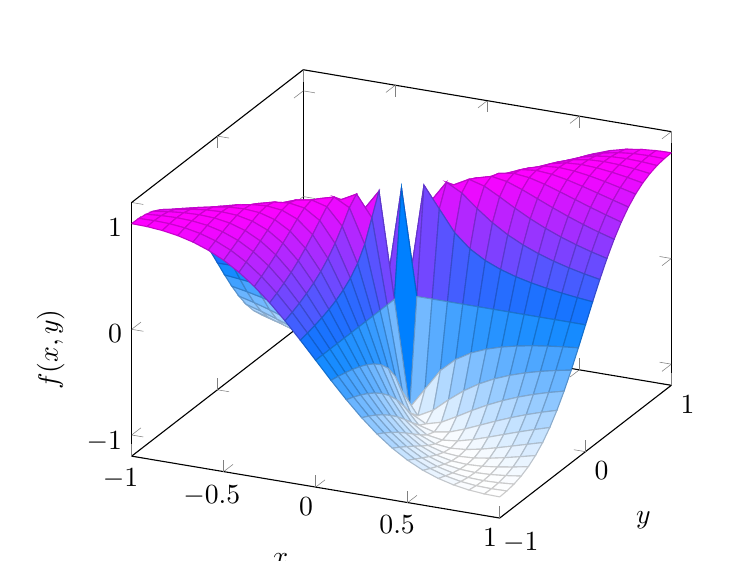
\begin{tikzpicture}
        \begin{axis}[xlabel = $x$,
            ylabel = $y$,
            zlabel = {$f(x,y)$},]
          \addplot3[domain=-1:1,y domain=-1:1, surf, colormap/cool] {2*x*y/(x^2 + y^2)};
          %\addplot3[domain=0.01:1,y domain=0.01:1, surf] {2*x*y/(x^2 + y^2)};
        \end{axis}
      \end{tikzpicture}
    \caption{Graf funkcije $f(x, y)$ iz zgleda \ref{zgl:1}.}
\end{figure}

\subsection{Preslikave iz $\R^n$ v $\R^m$}

Naj bo $D \subseteq \R^n$ in $f: D \subseteq \R^n \rightarrow \R^m$.
Koordinate $f(x_1, \dots, x_n)$ so torej funkcije na $D$. Zato velja 
$f(x_1, \dots, x_n) = (f_1 (x_1, \dots, x_n), \dots, f_m (x_1, \dots, x_n))$,
kjer so $f_j : D \rightarrow \R$ funkcije na $D$ za $j = 1, \dots, m$.
Seveda velja tudi obratno, saj $m$ funkcij $f_1, \dots, f_m$
določa preslikavo $f = (f_1, \dots, f_m)$ iz $D$ v $\R^m$.

\begin{trditev}
    Preslikava $f$ je zvezna v $a \in D$ natanko tedaj, ko so vse funkcije $f_1, \dots, f_n$ zvezne v $a$.
\end{trditev}

\begin{dokaz}
    $(\Rightarrow)$ Naj bo $\epsilon > 0.$
    Ker je $f$ zvezna v $a$, obstaja $\delta > 0$, da iz 
    $|x - a| < \delta$, $x \in D$ sledi $|f(x) - f(a)| < \varepsilon$.
    Torej iz $$|f(x) - f(a)| = \sqrt{(f_1 (x) - f_1 (a))^2 + \dots + (f_m (x) - f_m (a))^2} < \varepsilon$$
    dobimo $|f_j (x) - f_j (a)| < \varepsilon$ za vsak $j = 1, \dots, m$.
    Torej so vse funkcije $f_j$ zvezne v $a$.

    $(\Leftarrow)$ Denimo, da je za vsak $j$ funkcija zvezna v $a$.
    Torej obstaja $\delta_j$, da iz $|x - a| < \delta_j$, $x \in D$
    sledi $|f_j (x) - f_j (a)| < \frac{\varepsilon}{\sqrt{m}}$.
    Naj bo $\delta = \min \{\delta_1, \dots, \delta_m\}$ in sedaj je očitno,
    da je $f$ zvezna v $a$.
\end{dokaz}

Vsaka linearna preslikava $A: \R^n \rightarrow \R^m$ je zvezna na $\R^n$,
saj so vse njene koordinatne funkcije linearne oziroma polinomi prve stopnje.
To pa tudi implicira, da je vsaka linearna preslikava iz $\R^n$ v $\R^m$ omejena.
Lahko namreč pokažemo, da za $\forall x \neq 0$ velja $\frac{\|Ax\|}{\|x\|} < M$.
Naj bo $A = [a_{ij}]$ in $C = \max_{i, j} |a_{ij}|$.
Za vsako komponentno funkcijo $L_i (x) = a_{i1} x_1 + \dots + a_{in} x_n$ velja 
\begin{align*}
    |L_i (x)| &\leq |a_{i1}| |x_1| + \dots + |a_{in}| |x_n|\\
    &\leq C (|x_1| + \dots + |x_n|)\\
    &\leq C \sqrt{n} \|x\|,
\end{align*}
zaradi Cauchy-Schwartzove neenakosti.
Torej je $\|Ax\| = \sqrt{|L_1 (x)|^2 + \dots + |L_m (x)|^2} \leq C \sqrt{n \cdot m} \|x\|$
in tako imamo možno mejo $M = C \sqrt{m \cdot n}$.

\begin{opomba}
    Preslikave oblike $x \in \R^n \mapsto Ax + b \in \R^m$, kjer je $A$ matrika in $b \in \R^m$,
    so afine preslikave.
\end{opomba}

\subsection{Parcialni odvodi in diferenciabilnost}

Naj bo $D \subseteq \R^n$ in $f: D \rightarrow \R$ funkcija.
Naj bo $a = (a_1, \dots, a_n) \in D$ notranja točka, torej obstaja tak $r > 0$, da je 
$K(a, r) \subseteq D$. Tedaj je za vsak $j \in \{1, \dots, n\}$ funkcija 
$x_j \mapsto f(a_1, \dots, a_{j-1}, x_j, a_{j + 1}, \dots, a_n)$
definirana na $(a_j - r, a_j + r)$.

\begin{definicija}
    Naj bo $j \in \{1, \dots, n\}$. Če obstaja limita 
    $$\lim_{h \to 0} {\frac{f(a_1, \dots, a_{j-1}, a_j + h, a_{j+1}, \dots, a_n) - f(a)}{h}}$$
    oziroma če je funkcija $x_j \mapsto f(a_1, \dots, a_{j-1}, x_j, a_{j+1}, \dots, a_n)$
    odvedljiva v $a_j$, to limito imenujemo parcialni odvod funkcije $f$ po spremenljivki 
    $x_j$ v točki $a$ in ga označimo kot $\frac{\partial f}{\partial x} (a)$,
    $f_{x_j} (a)$ ali $(D_j f) (a)$.
\end{definicija}

\begin{zgled}
    Oglejmo si funkcijo $f(x, y) = x^2 y + \sin (x^2 + y^3)$.
    Njena parcialna odvoda sta $f_x (x, y) = 2 xy + 2x \cos (x^2 + y^3)$
    in $f_y (x, y) = x^2 + 3y^2 \cos (x^2 + y^3)$.
\end{zgled}

\begin{opomba}
    Obstoj parcialnih odvodov $f$ po vseh spremenljivkah v točki $a$ še ne pomeni, da je 
    funkcija v $a$ tudi zvezna (primer je zgled \ref{zgl:1}).
    Zahtevati moramo še omejenost vseh parcialnih odvodov v neki okolici točke $a$.
\end{opomba}

\begin{definicija}
    Funkcija $f: D \subseteq \R^n \rightarrow \R$ je v notranji točki $a \in D$
    diferenciabilna, če obstaja taka linearna funkcija $L: \R^n \rightarrow \R$,
    da je $f(a + h) = f(a) + L(h) + o(h)$, kjer je $\lim_{h \to 0} \frac{|o(h)|}{|h|} = 0$.
\end{definicija}

V standardnih koordinatah je vsaka linearna funkcija $L$ oblike $L(x) =l_1 x_1 + \dots + l_n x_n$, kar pa 
je ekvivalentno skalarnemu produktu vektorja $x$ z vektorjem $l = (l_1, \dots, l_n)$.
Spomnimo, da je pri $n = 1$ ta definicija ekvivalentna odvedljivosti $f$ v točki $a$.

Sedaj dokažimo, da če tak $L$ obstaja, je enolično določen. Denimo, da linearni funkciji $L_1, L_2$
ustrezata pogojema. Potem iz definicije diferenciabilnosti sledi $(L_1 - L_2) (h) = (o_1(h) - o_2 (h)) = o(h)$
in $\lim_{h \to 0} \frac{|o_1 (h)|}{|h|} = \lim_{h \to 0} \frac{|o_2 (h)|}{|h|} = 0$.
Torej je $\lim_{h \to 0} \frac{|o (h)|}{|h|} = 0$. Sedaj vzemimo tak $x \in \R^n$, da je $|x| = 1$ in naj bo $h = tx$ za $t > 0$.
Tedaj je $(L_1 - L_2) (h) = o(h)$ oziroma $(L_1 - L_2) (tx) = o (tx)$
in od tod $(L_1 - L_2) (x) = \frac{|o(tx)|}{|tx|}$ za $|x| = 1$.
Ker je $\lim_{h \to 0} \frac{|o(h)|}{|h|} = 0$, je tudi $\lim_{t \downarrow 0} \frac{|o (tx)|}{|tx|} = 0$
in zato je za vsak $|x| = 1$ $(L_1 - L_2) (x) = 0$. Torej je $L_1 - L_2 = 0$
oziroma $L_1 = L_2$ in $L$, če obstaja, je enolično določen.

\begin{opomba}
    $L= d_a f$ je diferencial funkcije $f$ v točki $a$ in funkcija $h \mapsto f(a) + d_a f(h)$
    je najboljša afina aproksimacija funkcije $h \mapsto f(a + h)$ v okolici točke $0$.
    To pa pomeni, da je $x \mapsto f(a) + d_a f(x-a)$ dobra aproksimacija $f(x)$ v okolici točke $a$.
\end{opomba}

\begin{izrek}
    Če je $f$ v notranji točki $a \in D$
    diferenciabilna, je v $a$ zvezna in parcialno odvedljiva na vse spremenljivke.
    V tem primeru je diferencial $f$ v točki $a$ oblike 
    $$(d_a f) (h) = \frac{\partial f}{\partial x_1} (a) h_1 + \dots + \frac{\partial f}{\partial x_n} (a) h_n.$$
\end{izrek}

\begin{opomba}
    Diferencial $d_a f$ lahko identificiramo z vektorjem $(\frac{\partial f}{\partial x_1} (a), \dots, \frac{\partial f}{\partial x_n} (a))$,
    ki ga imenujemo gradient funkcije $f$ v točki $a$. Tako velja 
    $$(d_a f) (h) = (\mathrm{\text{grad \(f\)}}) (a) \cdot h.$$
\end{opomba}

\begin{dokaz}
    Naj bo $f$ v $a \in D$ diferenciabilna, zato obstaja linearna funkcija $L: \R^n \rightarrow \R$,
    da velja $f(a + h) = f(a) + L(h) + o(h)$ in $\lim_{h \to 0} \frac{|o (h)|}{|h|} = 0$.
    Linearna funkcija $L$ je oblike $L(h) = l_1 h_1 + \dots + l_n h_n$, 
    kjer so $l_1, \dots, l_n \in \R$. Ker je $L$ linearna funkcija, je zvezna v $0$.
    Zato velja 
    \begin{align*}
        \lim_{h \to 0} f(a + h) &= \lim_{h \to 0} (f(a) + L(h) + o(h))\\
        &= f(a) + \lim_{h \to 0} L(h) + \lim_{h \to 0} o(h)\\
        &= f(a) 
    \end{align*}
    in $f$ je zvezna v $a$. Naj bo $h = (h_1, 0, \dots, 0)$.
    Potem je $|h| = |h_1|$. Za $h_1 \neq 0$ je 
    $\frac{f(a + h) - f(a)}{h_1} = \frac{L(h)}{h_1} + \frac{o(h)}{h_1} = l_1 + \frac{o (h)}{h_1}$
    in velja $\lim_{h_1 \to 0} \frac{f(a + h) - f(a)}{h_1} = l_1$.
    Torej obstaja parcialni odvod $\frac{\partial f}{\partial x_1} (a) = l_1.$
    Podobno sklepamo o obstoju ostalih parcialnih odvodov.
    Nazadnje smo tudi dokazali, da velja $(d_a f) (h) = \frac{\partial f}{\partial x_1} (a) h_1 + \dots + \frac{\partial f}{\partial x_n} (a) h_n.$
\end{dokaz}

Obrat trditve v splošnem ne velja, kar pokaže že primer $$f(x, y) = \begin{cases}
    \frac{2xy}{x^2 + y^2} ;& (x, y) \neq (0,0)\\
    0; & (x, y) = (0,0)
\end{cases},$$
katere oba parcialna odvoda v vsaki točki obstajata, a $f$ ni zvezna v $(0,0)$ in 
torej v tej točki tudi ni diferenciabilna. Lahko pa gremo še dlje in dokažemo, da tudi če je $f$ zvezna 
v neki točki in je tam tudi parcialno odvedljiva na vse spremenljivke, to še ne pomeni,
da je v tej točki tudi diferenciabilna. 

\begin{zgled}
    Oglejmo si funkcijo $$f(x, y) = \begin{cases}
        \frac{2xy}{\sqrt{x^2 + y^2}} ;& (x, y) \neq (0,0)\\
        0 ;& (x, y) = (0,0)
    \end{cases}.$$
    Tudi tukaj lahko z vpeljavo polarnih koordinat hitro dokažemo, da je $f$ zvezna v $(0,0)$.
    Ker velja $f(x, 0) = f(0, y) = 0$ za $\forall x, y \in \R$, obstajata parcialna odvoda $f_x (0,0) = f_y (0,0) = 0$ v točki $(0,0)$.
    Če bi bila $f$ torej diferenciabilna v $(0,0)$, je njen diferencial $d_{(0,0)} f(h) = 0.$
    Iz definicije diferenciabilnosti sledi $f(h) = f(0) + d_0 f(h) + o(h) = o(h)$ in posledično 
    $\lim_{h \to \infty} \frac{|f(h)|}{|h|} = 0.$ Sedaj pa vstavimo $h \neq 0$, $h = (r \cos \phi, r \sin \phi)$, $r > 0$ in dobimo 
    $\frac{|f(h)|}{|h|} = |\sin (2 \phi)|$, kar pa je odvisno le od parametra $\phi$.
    Limita $\lim_{h \to 0} \frac{|f(h)|}{|h|}$ ne obstaja, torej $f$ ni diferenciabilna v $(0,0)$,
    čeprav je tam zvezna in parcialno odvedljiva na obe spremenljivki.
\end{zgled}

\begin{izrek}
    Naj bo $f$ v okolici $a$ odvedljiva na vse spremenljivke in naj bodo
    parcialni odvodi zvezni v $a$. Potem je $f$ v $a$ diferenciabilna.
\end{izrek}

\begin{dokaz} [Dokaz za $n = 2$]
    Naj bo $f$ parcialno odvedljiva po $x$ in $y$ v okolici $(a, b)$.
    Naj bosta $h, k$ dovolj majhna, da je točka $(a + h, b + k)$
    v okolici $(a, b)$, kjer veljajo predpostavke izreka.
    Oglejmo si 
    \begin{align*}
        I &= f(a + h, b + k) - f(a, b)\\
        &=  f(a + h, b + k) - f(a, b + k) + f(a, b + k) - f(a, b).
    \end{align*}
    Sedaj dvakrat uporabimo Lagrangev izrek in dobimo $I = f_x(a^*, b + k) \cdot h + f_y (a, b^*) \cdot k$,
    kjer $a^*$ leži med $a$ in $a + h$ ter $b^*$ leži med $b$ in $b + h$.
    Zapišemo $f_x (a^*, b + k) = f_x (a, b) + \eta_1 (h, k)$ in $f_y (a, b^*) = f_y (a, b) + \eta_2 (h, k)$ in 
    ker sta parcialna odvoda $f_x, f_y$ zvezna v $(a, b)$, velja 
    $\lim_{(h, k) \to (0,0)} \eta_j (h, k) = 0$ za $j = 1, 2$.
    Sedaj definiramo $o(h, k) = \eta_1 (h, k) \cdot h + \eta_2 (h, k) \cdot k$.
    Naravno se zdi, da bomo kot kandidat za diferencial v $(a, b)$
    vzeli $(d_{(a, b)} f) (h, k) = f_x (a, b) \cdot h + \cdot f_y (a, b) \cdot k$.
    Preveriti moramo le še, da velja $\lim_{(h, k) \to (0, 0)} \frac{|o(h, k)|}{\sqrt{h^2 + k^2}} = 0.$
    To pa sledi iz trikotniške neenakosti:
    \begin{equation*}
        \frac{|o(h, k)|}{\sqrt{h^2 + k^2}} \leq \frac{|h|}{\sqrt{h^2 + k^2}} |\eta_1 (h, k)| + \frac{|k|}{\sqrt{h^2 + k^2}} |\eta_2 (h, k)| \leq |\eta_1 (h, k)| + |\eta_2 (h, k)| \qedhere 
    \end{equation*}
\end{dokaz}

\begin{opomba}
    Vse elementarne funkcije so diferenciabilne povsod, kjer so definirane.
\end{opomba}

\subsubsection{Višji parcialni odvodi}

Naj bo $f$ definirana v okolici $a \in \R^n$. Naj v tej okolici obstajajo 
njeni parcialni odvodi $\frac{\partial f}{\partial x_1}, \dots, \frac{\partial f}{\partial x_n}$.
Tako v okolici $a$ dobimo $n$ funkcij, ki pa so tudi lahko parcialno odvedljive:
tedaj obstajajo $\frac{\partial}{\partial x_1} \left(\frac{\partial f}{\partial x_1}\right) = \frac{\partial^2 d}{\partial x_1^2}$,
$\frac{\partial}{\partial x_2} \left(\frac{\partial f}{\partial x_1}\right) = \frac{\partial^2 d}{\partial x_2 \partial x_1}$,
$\frac{\partial}{\partial x_1} \left(\frac{\partial f}{\partial x_2}\right) = \frac{\partial^2 d}{\partial x_1 \partial x_2}$
in tako dalje.

\begin{zgled}
    Za primer vzemimo funkcijo $f(x, y) = x^2 y^3 + e^{x^4 y}$.
    Če začnemo izačunavati njene višje odvode,
    \begin{itemize}
        \item $f_x (x, y) = 2xy^3 + 4e^{x^4 y} (x^3 y)$
        \item $f_y (x, y) = 3x^2 y^2 + e^{x^4 y} x^4$
        \item $f_{xx} (x, y) = 2y^3 + 16 e^{x^4 y} (x^6 y^2) + 12 e^{x^4 y} x^2 y$
        \item $f_{xy} (x, y) = 6xy^2 + 4 e^{x^4 y} (x^7 y) + 4 e^{x^4 y} x^3$
        \item $f_{yx} (x, y) = 6xy^2 + 4 e^{x^4 y} (x^7 y) + 4 e^{x^4 y} x^3$
        \item $f_{yy} (x, y) = 6x^2 y + e^{x^4 y} x^8$
    \end{itemize}
    opazimo, da je $f_{xy} = f_{yx}$.
\end{zgled}

\begin{izrek}
    Naj bosta $\frac{\partial f}{\partial x_j}$ in $\frac{\partial f}{\partial x_i}$
    v okolici $a$ zvezna in naj na tej okolici obstajata $\frac{\partial}{\partial x_i} \left(\frac{\partial f}{\partial x_j}\right)$
    in $\frac{\partial}{\partial x_j} \left(\frac{\partial f}{\partial x_i}\right)$, ki sta zvezna v $a$.
    Tedaj velja $\frac{\partial}{\partial x_i} \left(\frac{\partial f}{\partial x_j}\right) = \frac{\partial}{\partial x_j} \left(\frac{\partial f}{\partial x_i}\right)$.
\end{izrek}

\begin{opomba}
    V tem primeru rečemo, da parcialni odvodi komutirajo oziroma velja $D_i \cdot D_j = D_j \cdot D_i.$
\end{opomba}

\begin{dokaz}
    Dovolj je, da dokažemo za primer, ko je $n = 2$,
    saj so pri parcialnih odvodih ostale spremenljivke konstantne.
    Naj bo $f$ definirana v okolici $(a, b)$ in naj tam obstajata $f_x, f_y$, ki sta zvezna v tej okolici.
    Predpostavimo še, da na tej okolici obstajata tudi $(f_x)_y$ in $(f_y)_x$, ki sta zvezna v $(a, b)$.
    Za dovolj majhna $(h, k)$ si oglejmo izraz $$I = f(a+h, b + k) - f(a, b+ k) - f(a + h, b) + f(a, b).$$
    Naj bo $\phi(x) = f(x, b + k) - f(x, b)$. Tedaj je $I = \phi(a + h) - \phi(a) = \phi'(a^*) \cdot h$
    kjer smo uporabili Lagrangev izrek in je $a^*$ med $a$ in $a + h$. Od tod naprej pa je
    $\left(f_x (a^*, b + k) - f_x (a^*, b)\right) h = (f_x)_y (a^*, b^*) hk$
    za nek $b^*$ med $b$ in $b + k$.
    Sedaj pa definirajmo $\psi(y) = f(a + h,y) - f(a, y)$ in po podobnem razmisleku 
    dobimo $I = (f_y)_x (a^{**}, b^{**}) hk$, kjer je $b^{**}$ med $b$ in $b + k$ 
    in $a^{**}$ med $a$ in $a + h$.
    Tako imamo $(f_y)_x (a^{**}, b^{**})= (f_x)_y (a^*, b^*)$. Ko pošljemo $(h, k) \to (0,0)$
    in upoštevamo zveznost $(f_x)_y$ in $(f_y)_x$ v $(a, b)$, dobimo enakost.
\end{dokaz}

\begin{opomba}
    Če so prvi parcialni odvodi zvezni, je funkcija diferenciabilna.
    Če so drugi parcialni odvodi zvezni, so mešani odvodi enaki.
    Če so tudi tretji odvodi zvezni, so tudi vsi mešani tretji odvodi enaki,
    saj so tretji odvodi hkrati drugi odvodi prvih odvodov. 
    To se nadaljuje v neskončnost.
\end{opomba}

\begin{definicija}
    Naj bo $D$ odprta podmnožica na $\R^n$. Vektorski prostor vseh $k$-krat ($k \in \N$)
    zvezno parcialno odvedljivih funkcij na $D$ označimo s $C^k(D)$.
    Prostor gladkih funkcij na $D$ je $C^{\infty} (D) = \bigcap_{k = 1} ^\infty C^k (D)$,
    prostor zveznih funkcij na $D$ pa je $C(D)$.
\end{definicija}

To pomeni, da je $f \in C^k (D)$, če obstajajo vsi parcialni odvodi funkcije $f$ 
do reda $k$ in so zvezne funkcije na $D$.

\subsection{Diferenciabilnost preslikav iz $\R^n$ v $\R^m$}

Naj bo $D \subseteq \R^n$ in $F: D \rightarrow \R^m$
preslikava. Naj bo $a$ notranja točka $D$ oziroma naj bo $F$ definirana 
v okolici točke $a$.

\begin{definicija}
    Preslikava $F$ je diferenciabilna v točki $a$, 
    če obstaja taka linearna preslikava $A: \R^n \to \R^m$, 
    da je $F(a + h) = F(a) + A(h) + o(h),$ kjer je $\lim_{h \to 0} \frac{|o(h)|_m}{|h|_n} = 0.$
\end{definicija}

\begin{opomba}
    Kot pri funkcijah vidimo, da je tak $A$, če obstaja, enolično določen.
    To je diferencial $F$ v točki $a$ in ga označimo z $d_a F$ ali $(DF) (a)$.
\end{opomba}

\begin{zgled}
    Oglejmo si nekaj primerov diferencialov funkcij.
    \begin{itemize}
        \item Naj bo $A: \R^n \to \R^m$ matrika in $F(x) = Ax$.
        Ker je $F(a + h) = A(a + h) = Aa + Ah = F(a) + Ah$, je $(DF)(a) = A$ 
        za $\forall a \in \R^n$.
        \item Naj bo $F: \R^{n \times n} \to \R^{n \times n}$ s predpisom $X \mapsto X^2$.
        Potem je $F(A + H) = A^2 + AH + HA + H^2$ in preslikava $H \mapsto AH + HA$ je linearna na $\R^{n \times n}$.
        Hkrati pa preslikava $H \mapsto H^2$ ustreza pogojem, saj po Cauchy-Schwartzovi neenakosti velja $|A \cdot B| \leq |A| \cdot |B|$ in torej velja $\lim_{H \to 0} \frac{|H^2|}{|H|} \leq \lim_{H \to 0} |H| = 0$.
        Torej je $H \mapsto AH + HA$ res diferencial $F$ v $A$.
    \end{itemize}
\end{zgled}

Naj bo preslikava $F = (f_1, \dots, f_m)$, kjer so $f_1, \dots, f_m$ funkcije $n$ spremenljivk,
definirane v okolici $a$.

\begin{izrek}
    Preslikava $F$ je diferenciabilna v $a$ natanko tedaj, 
    ko so $f_1, \dots, f_m$ diferenciabilne v $a$.
    V tem primeru velja 
    $$(DF) (a) = \begin{bmatrix}
        (D f_1) (a)\\
        \vdots\\
        (Df_m) (a)
    \end{bmatrix} = \begin{bmatrix}
        \frac{\partial f_1}{\partial x_1} (a) & \cdots & \frac{\partial f_1}{\partial x_n} (a)\\
        \vdots & & \vdots\\
        \frac{\partial f_m}{\partial x_1} (a) & \cdots & \frac{\partial f_m}{\partial x_n} (a)
    \end{bmatrix}.$$
\end{izrek}

\begin{posledica}
    Če so vsi parcialni odvodi funkcij $f_1, \dots, f_m$ zvezni v $a$, je $F = (f_1, \dots, f_m)$
    diferenciabilna v točki $a$.
\end{posledica}

\begin{dokaz}
    $(\Rightarrow)$ Naj bo $F$ diferenciabilna v $a$. Torej obstaja linearna preslikava
    $A: \R^n \to \R^m$, da je $F(a + h) = F(a) + A(h) + o(h)$.
    Naj bo $$A = \begin{bmatrix}
        A_{11} (a) & \cdots & A_{1n} (a)\\
        \vdots & & \vdots\\
        A_{m1} (a) & \cdots & A_{mn} (a)
    \end{bmatrix}$$
    in $o(h) = (o_1 (h), \dots, o_m (h))$.
    Če sedaj gledamo prejšnjo enačbo po komponentah, dobimo za vsak $j \in \{1, \dots, m\}$ zvezo 
    $$f_j (a + h) = f_j (a) + (A_{j1} h_1 + \dots + A_{jn} h_n) + o_j (h).$$
    Ker je preslikava $h \to A_{j1} h_1 + \dots + A_{jn} h_n$ linearna in je 
    $\lim_{h \to 0} \frac{|o_j(h)|}{|h|} \leq \lim_{h \to 0} \frac{\sqrt{o_1^2 (h) + \dots + o_m^2 (h)}}{|h|} = \lim_{h \to 0} \frac{|o_j(h)|}{|h|} = 0$,
    je $f_j$ diferenciabilna in njen diferencial 
    $$(d_a f_j) (h) = A_{j1} h_1 + \dots + A_{jn} h_n.$$
    Trditev v obratno smer $(\Leftarrow)$ je podoben.
\end{dokaz}

\begin{izrek}[Verižno pravilo]
    Naj bosta $D \subseteq \R^n$ in $\Omega \subseteq \R^m$.
    Naj bo $a$ notranja točka $D$ in naj bo $b$ notranja točka $\Omega$.
    Naj bo $F: D \to \Omega$, $F(a) = b$, diferenciabilna v $a$.
    Naj bo $G: \Omega \to \R^k$ diferenciabilna v $b$. Tedaj je $\Phi = G \circ F$ diferenciabilna 
    v $a$ in velja $(D \Phi) (a) = (DG) (F(a)) \cdot (DF) (a)$ oziroma zapisano z matrikami:
    \begin{equation*}
        (D \Phi) (a) = \begin{bmatrix}
            \frac{\partial g_1}{\partial y_1} (b) & \cdots & \frac{\partial g_1}{\partial y_m} (b)\\
            \vdots & & \vdots\\
            \frac{\partial g_k}{\partial y_1} (b) & \cdots & \frac{\partial g_k}{\partial y_m} (b)
        \end{bmatrix}
        \begin{bmatrix}
            \frac{\partial f_1}{\partial x_1} (a) & \cdots & \frac{\partial f_1}{\partial x_n} (a)\\
            \vdots & & \vdots\\
            \frac{\partial f_m}{\partial x_1} (a) & \cdots & \frac{\partial f_m}{\partial x_n} (a)
        \end{bmatrix}
    \end{equation*}
\end{izrek}

\begin{posledica} \label{pos:1}
    Oglejmo si primer $k = 1$, kjer je $g$ funkcija.
    Naj bo diferenciabilna v okolici $\Omega$ točke $b$.
    Naj bo $F = (f_1, \dots, f_m)$ diferenciabilna preslikava v okolici $D$ točke $a$,
    torej imamo $F: D \to \Omega$ in $F(a) = b$.
    Tedaj je funkcija $\Phi(x_1, \dots, x_n) = g(f_1(x_1, \dots, x_n), \dots, f_m(x_1, \dots, x_n))$
    diferenciabilna v $a$ in velja 
    $$\frac{\partial \Phi}{\partial x_j} = \frac{\partial g}{\partial y_1} (b) \frac{\partial f_1}{\partial x_j} (a) + \dots + \frac{\partial g}{\partial y_m} (b) \frac{\partial f_m}{\partial x_j} (a).$$
\end{posledica}

\begin{dokaz}
    Vemo, da velja $F(a + h) = F(a) + (DF)(a)h + o_F (h)$ in $G(b + k) = G(b) + (DG) (b) k + o_G (k)$,
    kjer je $\lim_{h \to 0} \frac{|o_F (h)|}{|h|} = 0$ ter $\lim_{k \to 0} \frac{|o_G (k)|}{|k|} = 0$.
    Sedaj v drugo enačbo vstavimo $F(a) = b$ in $k = (DF)(a)h + o_F (h)$ in poračunamo.
    Dokazali bomo, da je linearna preslikava $h \mapsto (DG)(b) (DF) (a) h$, ki jo s tem dobimo, res diferencial.
    To pomeni, da moramo za $$o(h) = (DG) (b) o_F (h) + o_G ((DF) (a) h + o_F (h))$$ preveriti, 
    če res velja $\lim_{h \to 0} \frac{|o(h)|}{|h|}$. Linearna preslikava $(DG) (b)$ je omejena in obstaja $M$,
    da je $|(DG) (b) \cdot v| \leq M|v|$, $\forall v$. Torej je $0 \leq \frac{|(DG) (b) \cdot o_F (h)|}{|h|} \leq M \frac{|o_F(h)|}{|h|}$ 
    in $\lim_{h \to 0} \frac{|(DG) (b) \cdot o_F (h)|}{|h|} = 0$.
    Naj bo sedaj $\varepsilon > 0$. Potem obstaja $\delta > 0$, da za $|k| < \delta$ velja $|o_G (k)| < \varepsilon |k|$.
    Ker je $\lim_{h \to 0} ((DF)(a)h + o_F(h)) = 0$, obstaja $\delta_1 > 0$, da za $|h| < \delta_1$ velja
    $|(DF)(a)h + o_F(h)| < \delta$ in posledično $|o_G ((DF)(a)h + o_F(h))| < \varepsilon |(DF)(a)h + o_F(h)|$.
    Iz omejenosti linearnih preslikav pa za $|h| < \delta_1$ sledi $$\frac{|o_G ((DF)(a)h + o_F(h))|}{|h|} < \varepsilon \frac{|(DF)(a)h + o_F(h)|}{|h|} < \varepsilon \left(M_1 + \frac{|o_F (h)|}{|h|}\right).$$
    To pa že implicira $\lim_{h \to 0} \frac{|o(h)|}{|h|}$.
\end{dokaz}

\begin{definicija}
    Naj bo $D \subseteq \R^n$ odprta. Preslikava $F: D \to \R^m$ je $C^k$, če so vse njene komponentne funkcije $C^k$.
\end{definicija}

\subsection{Izrek o implicitni funkciji}

Motivacija za ta razdelek je iskanje nekega zadostnega pogoja za enačbo $f(x, y) = 0$,
ki nam bo zagotovil, da v okolici neke točke $(a, b)$ za vsak $x$ blizu $a$ obstaja natanko določen $y = \phi(x)$ blizu $b$,
ki reši enačbo $f(x, \phi(x)) = 0$. Ta funkcija $\phi(x)$ je z enačbo $f(x, y) = 0$ implicitno podana funkcija spremenljivke $x$.
Včasih v okolici $(a, b)$ morda take funkcije ni in takrat se vprašamo, ali lahko rešimo enačbo $f(x, y) = 0$
na $x$ kot funkcijo $y$-a.

\begin{zgled}
    Izrek o implicitni funkciji se bo ohlapno navezoval na naslednja primera.
    \begin{itemize}
        \item Linearen primer: $ax + by = c$, kjer so $a,b,c \in \R$.
        Potreben in zadosten pogoj, da to enačbo lahko razrešimo na $x$, je $b \neq 0$.
        Opazimo lahko tudi, da je v tem primeru $b$ kar parcialni odvod po $y$.
        \item Nekatere enačbe nimajo rešitev: primer je recimo $x^2 + y^2 + 1 = 0$.
        Če torej želimo upati, da bomo enačbo lahko razrešili na $y$ kot funkcijo $x$-a,
        potrebujemo na začetku vsaj kakšno rešitev $(a, b)$, da je $f(a, b) = 0.$
    \end{itemize}
\end{zgled}

\begin{izrek}[Osnovna oblika izreka o implicitni funkciji]
    Naj bo $D \subseteq \R^2$ odprta množica. Naj bo $f \in C^1 (D)$.
    Naj bo $(a, b) \in D$ taka, da velja $f(a, b) = 0$ in $f_y (a, b) \neq 0$.
    Tedaj obstajata okolici $I = (a - \delta, a + \delta)$ in $J = (b - \varepsilon, b + \varepsilon)$,
    $\delta, \varepsilon > 0$, da je $I \times J \subseteq D$ ter za vsak 
    $x \in I$ obstaja natanko določen $y =\phi (x) \in J$, da velja 
    $f(x, \phi(x)) = 0.$
    Funkcija $\phi: I \to J$ je torej enolično določena funkcija, za katero velja:
    \begin{itemize}
        \item $\phi(a) = b$,
        \item $f(x, \phi(x)) = 0$, $\forall x \in I$,
        \item $\phi \in C^1 (I)$ in $\phi' (x) = - \frac{f_x (x, \phi(x))}{f_y (x, \phi(x))}$.
    \end{itemize}
\end{izrek}

\begin{opomba}
    Če je $f \in C^k (D)$, potem je tudi $\phi \in C^k (I)$.
\end{opomba}

\begin{dokaz}
    Vemo, da je $f \in C^1 (D)$, zato je $f_y \in C(D)$.
    Brez škode za splošnost predpostavimo $f_y (a, b) > 0$.
    Potem obstaja okolica točke $(a, b)$ $\overline{I}_1 \times \overline{J} \subseteq D$,
    kjer sta $I_1 = (a - \delta_1, a + \delta_1)$ in $J = (b - \varepsilon, b + \varepsilon)$ za 
    $\delta_1, \varepsilon > 0$, tako da je $f_y > 0$ na $\overline{I}_1 \times \overline{J}$.
    Pri fiksnem $x \in I_1$ je funkcija $y \mapsto f(x, y)$ strogo naraščajoča na $J$.
    Ker je $f(a, b) = 0$, je $f(a, b + \varepsilon) > 0$ in $f(a, b - \varepsilon) < 0$.
    Zaradi zveznosti obstaja $0 < \delta < \delta_1$, da je $f(x, b + \varepsilon) > 0$ in $f(x, b - \varepsilon) < 0$
    za $x \in I = (a - \delta, a + \delta)$.
    Za vsak $x \in I$ je funkcija $y \mapsto f(x, y)$ strogo naraščajoča na $J$ in na 
    krajiščih nasprotno predznačena, zato ima na $J$ natanko eno ničlo.
    Označimo jo s $\phi (x) = y$.
    Torej je $\phi: I \rightarrow J$ enolično določena funkcija, za katero veljata prvi dve lastnosti, ki smo ju navedli v besedilu izreka.
    Dokazati moramo še, da je ta funkcija zvezno odvedljiva.
    Naj bosta $x, x + \varDelta x \in I$ in $\phi(x) = y,\ \phi(x + \varDelta x) = y + \varDelta y$.
    Sedaj imamo 
    \begin{align*}
        0 &= f(x + \varDelta x, y + \varDelta y) - f(x, y)\\
        &= f(x + \varDelta x, y + \varDelta y) - f(x + \varDelta x, y) + f(x + \varDelta x, y) - f(x, y)\\
        &= f_y (x + \varDelta x, y^*) \varDelta y + f_x (x^*, y) \varDelta x,
    \end{align*}
    za nek $y^*$ med $y$ in $y + \varDelta y$ ter $x^*$ med $x$ in $x + \varDelta$.
    Od tod sledi $\varDelta y = - \frac{f_x (x^*, y)}{f_y (x + \varDelta x, y^*)} \varDelta x$.
    Ker je $\overline{I} \times \overline{J} \subseteq D$ kompakt in $f_x, f_y$ na njej zvezni funkciji,
    na tem območju zavzameta maksimume in minimume. To implicira $\lim_{\varDelta x \to 0} \varDelta y = 0$,
    torej je $\phi(x)$ zvezna na $I$. Na koncu pa sledi podoben razmislek še za odvod:
    \begin{equation*}
        \lim_{\varDelta x \to 0} \frac{\varDelta y}{\varDelta x} 
        = \lim_{\varDelta x \to 0} \left( -\frac{f_x (x^*, y)}{f_y (x + \varDelta x, y^*)} \right)
        \stackrel{\text{zveznost}}{=} - \frac{f_x (x, y)}{f_y (x, y)} \qedhere
    \end{equation*}
\end{dokaz}

\begin{opomba}
    Če bi vedeli, da je $\phi$ odvedljiva, bi lahko njen odvod izračunali s pomočjo verižnega pravila iz posledice \ref{pos:1}.
    Če odvajamo $f(x, \phi(x)) = 0$, dobimo $f_x (x, \phi(x)) + f_y (x, \phi(x)) \cdot \phi'(x) = 0$.
\end{opomba}

\begin{zgled}
    V nekaterih primerih lahko najdemo iskano funkcijo $\phi$, tudi če pogoji iz izreka niso izpolnjeni.
    \begin{itemize}
        \item Naj bo $f(x, y) = y^3 - x = 0$. V izhodišču je $f(0,0) = 0$ in $f_y (0,0) = 0$,
        kljub temu pa obstaja rešitev $y (x) = x^\frac{1}{3}$ (ki ni odvedljiva).
        \item Naj bo $f(x, y) = y^2 - x^2 - x^4 = 0$, $f(0,0) = 0$, $f_y (0,0) = 0$.
        Potem imamo dve rešitvi v okolici izhodišča: $f_1 = x \sqrt{1 + x^2}$ in $f_2 = - x \sqrt{1 + x^2}$.
    \end{itemize}
\end{zgled}

Sedaj si lahko naše vprašanje zastavimo splošneje.
Predpostavimo, da imamo preslikavo $n + m$ spremenljivk,
ki jo sestavlja $m$ koordinatnih funkcij (enačb).
Pričakujemo, da bomo lahko $m$ spremenljivk izrazili kot funkcije ostalih $n$ spremenljivk.
Kot poprej si najprej oglejmo linearni model $Ax + By = b$, kjer je $x \in \R^n$, $y \in \R^m$ in $b \in \R^m$.
Tedaj mora $A$ biti $m \times n$ matrika, $B$ pa $m \times m$ matrika.
Zadostni pogoj, ki zagotovi, da ta sistem lahko razrešimo na $y$, je zahteva, da je $B$ obrnljiva matrika
oz. $\det B \neq 0$. Tedaj je $y = B^{-1} (b - Ax)$.
Poseben primer je, ko vzamemo $n = 0$.
Takrat je naša enačba $By = b$ rešljiva za poljubno desno stran $B$ natanko tedaj, ko je $B$ obrnljiva.

\begin{definicija}
    Naj bosta $D, \Omega \subseteq \R^n$ odprti množici. Preslikava $F: D \rightarrow \Omega$
    je difeomorfizem, če je:
    \begin{enumerate}
        \item bijekcija,
        \item razreda $C^1$ na $D$ in 
        \item inverzna preslikava $F^{-1} :\Omega \to D$ je razreda $C^1$ na $\R$.
    \end{enumerate}
\end{definicija}

\begin{trditev}
    Če je $F: D \to \Omega$ difeomorfizem, je $(DF) (x)$ obrnljiva za vsak $x \in D$ in velja 
    $(DF^{-1}) (y) = (DF)^{-1} (x)$, kjer je $y = F(x)$.
\end{trditev}

\begin{dokaz}
    Velja $F^{-1} \circ F = Id$.
    To odvajamo in po verižnem pravilu dobimo 
    $(DF^{-1}) (F(x)) \cdot (DF) (x) = I$.
    Torej je $(DF)(x)$ obrnljiva in velja $(DF^{-1}) (y) = (DF)^{-1} (x)$.
\end{dokaz}

\begin{posledica}
    Potreben pogoj, da je $F: D \rightarrow \Omega$ difeomorfizem, je $\det (DF) (x) \neq 0$
    za $\forall x \in D$.
\end{posledica}

\begin{zgled}
    Obrat v splošnem ne velja za $F: \R^2 \to \R^2$ s predpisom
    $F(x, y) = (e^x \cos y, e^x \sin y)$. 
    Ta preslikava ima obrnljiv inverz, saj je 
    $$(DF) (x, y) = \begin{bmatrix}
        e^x \cos y & - e^x \sin y\\
        e^x \sin y & e^x \cos y
    \end{bmatrix}$$
    in $\det (DF)(x, y) = e^{2x} \neq 0$.
    Vendar pa $F$ ni difeomorfizem, saj velja $F(x, y + 2 \pi) = F(x, y)$ in $F$ ni bijekcija.
\end{zgled}

Kljub temu pa bomo pokazali, da obrat zgornje trditve velja lokalno.

\begin{izrek}[o inverzni funkciji]
    Naj bo $D \subseteq \R^n$ odprta in $F: D \to \R^n$ preslikava razreda $C^1$.
    Naj bo $a \in D$ in naj bo $\det (DF) (a) \neq 0$.
    Tedaj obstaja okolica $U$ točke $a$ v $D$ in okolica $V$ točke $b = F(a)$ v $\R^n$, da je 
    $F: U \to V$ difeomorfizem.
\end{izrek}

Dodatek tega izreka je, da če je $F \in C^k (D)$, je 
tudi $F^{-1} \in C^k$ za neko naravno število $k$. To sledi iz relacije $(DF^{-1}) (y) = (DF)^{-1} (F^{-1} (y))$.
Denimo, da je $F \in C^2 (D)$. Potem je po izreku $F^{-1} \in C^1 (V)$, torej je $y \mapsto (DF)^{-1} (F^{-1} (y))$
tudi $C^1$ (koeficienti inverzne matrike so kar polinomi koeficientov prvotne matrike, deljeni z determinanto).
Potem pa je tudi $y \mapsto (DF^{-1}) (y)$ $C^1$ preslikava in zato je $F^{-1} \in C^2 (V)$.
Za višje $k \in \N$ je enak sklep z indukcijo.

\begin{opomba}
    Če je $F: D \to \Omega$ taka, da je $\det (DF) (x) \neq 0$ na $D$, rečemo, da je $F$ lokalni difeomorfizem.
\end{opomba}

\begin{opomba}
    Pri dokazu izreka o inverzni preslikavi bomo uporabili predpostavke, da je $a = b = 0$ in $(DF) (0) = I$,
    ki jih dosežemo, če opazujemo preslikavo $x \mapsto (DF)^{-1} (a) (F(x + a) - F(a)) = G(x)$.
    Če pokažemo izrek za $G$, ga dokažemo za $F(x) = (DF) (a) G(x - a) + F(a)$.
\end{opomba}

Preden se lotimo dokaza izreka o inverzni preslikavi, bomo zapisali izrek o implicitni funkciji in ga dokazali 
s pomočjo izreka o inverzni preslikavi.
Naj bo $D \subseteq \R^n \times \R^m$ odprta množica. Naj bo $F: D \rightarrow \R^m$ $C^1$ preslikava,
$x = (x_1, \dots, x_n) \in \R^n$, $y \in (y_1, \dots, y_m) \in \R^m$ in $F = (f_1, \dots, f_m)$.
Rešujemo sistem enačb $F(x, y) = 0$ oziroma:
\begin{align*}
    f_1 &(x_1, \dots, x_n, y_1, \dots, y_m) = 0\\
    f_2 &(x_1, \dots, x_n, y_1, \dots, y_m) = 0\\
    \vdots & \\
    f_m & (x_1, \dots, x_n, y_1, \dots, y_m) = 0.
\end{align*}
Definirajmo še odvod preslikave $F$ po spremenljivkah $x$ in $y$.
Odvod po $x$, ki ga označimo kot $\frac{\partial F}{\partial x} (x, y) = (D_x F) (x, y)$,
je enak odvodu (če ta obstaja) preslikave $x \mapsto F(x, y)$ pri fiksnem $y$.
Podobno definiramo še $\frac{\partial F}{\partial y} = (D_y F) (x, y)$ in dobimo
\begin{equation*}
    (D_x F) (x, y) = \begin{bmatrix}
        \frac{\partial f_1}{\partial x_1} & \cdots & \frac{\partial f_1}{\partial x_n}\\
        \vdots & & \vdots\\
        \frac{\partial f_m}{\partial x_1} & \cdots & \frac{\partial f_m}{\partial x_n}
    \end{bmatrix} (x, y), \qquad 
    (D_y F) (x, y) = \begin{bmatrix}
        \frac{\partial f_1}{\partial y_1} & \cdots & \frac{\partial f_1}{\partial y_m}\\
        \vdots & & \vdots\\
        \frac{\partial f_m}{\partial xy_1} & \cdots & \frac{\partial f_m}{\partial y_m}
    \end{bmatrix} (x, y).
\end{equation*}

\begin{opomba}
    Celoten odvod $F$ se izraža s parcialnima odvodoma (če celoten odvod obstaja, obstajata tudi parcialna odvoda),
    in sicer kot matrika v bločnem zapisu $(DF)(x, y) = \begin{bmatrix}
        (D_x F) (x, y) & (D_y F) (x, y)
    \end{bmatrix}$.
    Od tod sledi $$(DF) (x, y) \begin{bmatrix}
        h\\ k
    \end{bmatrix} = (D_x F) (x, y) h + (D_y F) (x, y) k.$$
\end{opomba}

\begin{izrek}[o implicitni preslikavi]
    Naj bo $D \subseteq \R^n \times \R^m$ odprta množica.
    Naj bo $(a, b) \in D$ in naj bo $F: D \to \R^m$ taka $C^1$ preslikava, da je
    $F(a, b) = 0$ in $\det (D_y F) (a, b) \neq 0$.
    Potem obstaja okolica $U$ točke $a \in \R^n$ in okolica $V$ točke $b \in \R^m$,
    da je $U \times V \subseteq D$, ter taka enolično določena $C^1$ preslikava $\phi: U_x \to V_j$, da je 
    \begin{enumerate}
        \item $\phi (a) = b$,
        \item $F(x, y) = 0 \Leftrightarrow y = \phi (x)$ za $(x, y) \in U \times V$.
        \item $(D \phi) (x) = - (D_y F)^{-1} (x, y) (D_x F) (x, y)$, kjer je $y = \phi (x)$.
    \end{enumerate}
\end{izrek}

Tudi pri tem izreku lahko upoštevamo dodatek, da če je $F \in C^k (D)$, je tudi $\phi \in C^k (U)$ 
za $k \in \N$.

\begin{dokaz}
    Definirajmo preslikavo $\Phi: D \subseteq \R^n \times \R^m \to \R^n \times \R^m$ s predpisom $(x, y) \mapsto (x, F(x, y))$.
    $\Phi$ je razreda $C^1$ in odvod $\Phi$ v $(a, b)$ je 
    $$(D \Phi) (a, b) = \begin{bmatrix}
        I_{\R^n} & 0\\
        (D_x F) (a, b) & (D_y F) (a, b)
    \end{bmatrix}$$
    in $\det (D \Phi) (a, b) = \det (D_y F) (a, b) \neq 0$.
    Po izreku o inverzni preslikavi obstaja okolica $\mathcal{U}$ točke $(a, b)$ v $\R^n \times \R^m$ ter 
    okolica $\mathcal{V}$ točke $(a, 0) = \Phi(a, b)$ v $\R^n \times \R^m$, da je $\Phi: \mathcal{U} \to \mathcal{V}$ 
    difeomorfizem. Brez škode za splošnost lahko prevzamemo $\mathcal{U} = U_1 \times V$, kjer je 
    $U_1$ okolica $a$ v $\R^n$ in $V$ okolica $b$ v $\R^m$.
    Ker je $\Phi$ oblike $(x, y) \to (x, F(x, y))$, je inverz $\Phi^{-1}$ oblike $(x, w) \to (x, G(x, w))$
    in $G$ je $C^1$.
    Prav ta preslikava je kandidat za $\phi(x) = G(x, 0)$, ki pa morda ni definirana na okolici $U_1$.
    Res, naj bo $U$ okolica $a$ v $\R^n$, da za vsak $x \in U$ velja $(x, 0) \in \mathcal{V}$.
    Sedaj definiramo $C^1$ preslikavo $\phi: U \to V$ s predpisom $\phi (x) = G(x, 0)$, 
    za katero veljata prvi dve navedeni lastnosti iz izreka. Odvod pa preverimo tako, 
    da odvajamo obe strani enačbe $F(x, \phi(x)) = 0$ za $x \in U$ in dobimo 
    $D_x F + D_y F \cdot D \phi = 0$ ter od tod 
    \begin{equation*}
        (D\phi) (x) = - (D_y F)^{-1} (x, \phi (x)) (D_x F) (x, \phi(x)). \qedhere
    \end{equation*}
\end{dokaz}

\begin{zgled}
    Vzemimo funkciji $f(x, y, z) = y + yz + xz^2$ in $g(x, y, z) = z + zy + x^2$.
    Vidimo, da je $f(0,0,0) = g(0,0,0) = 0$.
    Če odvajamo, dobimo $f_y (x, y, z) = 1 + x$, $f_z (x, y, z) = 2xz$, $g_y = z$ in $g_z (x, y, z) = 1 + y$.
    V točki $(0,0,0)$ dobimo matriko $$\begin{bmatrix}
        1 & 0\\
        0 & 1
    \end{bmatrix},$$
    torej obstajata gladki funkciji $\phi(x)$ in $\psi (x)$, ki sta definirani v okolici $0$
    in za vsak $x$ iz te okolice rešita sistem, hkrati pa velja $\phi(0) = \psi (0) = 0$.
    Če ti dve funkciji še odvajamo v točki $x = 0$, dobimo:
    \begin{gather*}
        \frac{d}{dx} (y + xy + xz^2) = y' + xy' + y + z^2 + 2zxz' = 0\\
        \frac{d}{dx} (z + zy + x^2) = z' + z'y + z y' + 2x = 0.
    \end{gather*}
    V točki $(0,0,0)$ dobimo $y' = \phi'(0) = 0$ in $z' = \psi' (0) = 0$.
    Če odvajamo še enkrat, v $(0,0,0)$ dobimo $\phi'' (0) = 0$ in $\psi'' (0) = -2$.
    Torej imamo Taylorjev razvoj za $\phi$ in $\psi$ do členov 2. reda: $\phi(x) = o_\phi (x^2)$ in $\psi(x) = - x^2 + o_\psi (x^2)$.
\end{zgled}

\begin{opomba}
    Matrika prvih odvodov $DF = \left(\frac{\partial f_j}{\partial x_i}\right)$ se imenuje Jacobijeva matrika.
    Če je kvadratna, pa se njeni determinanti reče Jacobijeva detereminanta.
    Ta bo igrala pomembno vlogo pri vpeljavi novih spremenljivk v $n$-terni integral.
\end{opomba}

\begin{lema}
    Obstaja $r > 0$, da za vsak par $x_1, x_2 \in \overline{K(0, r)} \subseteq D$ velja 
    $$|H(x_1) - H(x_2)| \leq \frac{1}{2} |x_1 - x_2|.$$
\end{lema}

\begin{dokaz}[Dokaz izreka o inverzni preslikavi]
    Omenili smo že redukcijo na primer $F(0) = 0$ in $DF(0) = I$.
    Torej je $F$ oblike $F(x) = x + H(x)$, kjer $H$ slika iz okolice $a \in \R^n$ v $\R^n$
    in velja $H(0) = 0$ in $(DH)(0) = 0$.
    Uporabimo lemo in $r$ še nekoliko zmanjšamo, da na $\overline{K(0, r)}$ velja $\det (DF) (x) \neq 0$.
    Najprej dokažimo injektivnost $F: \overline{K(0, r)} \to \R^n$. Za $x_1, x_2 \in \overline{K(0, r)}$ velja 
    \begin{align*}
        |F(x_1) - F(x_2)| &= |x_1 + H(x_1) - x_2 - H(x_2)|\\
        &\geq |x_1 - x_2| - |H(x_1) - H(x_2)|\\
        &\geq \frac{1}{2} |x_1 - x_2|
    \end{align*}
    in torej iz $x_1 \neq x_2$ sledi $F(x_1) \neq F(x_2)$.
    Od tod sledi zveznost $F^{-1}: F(\overline{K(0, r)}) \to \overline{K(0, r)}$,
    saj velja $|y_1 - y_2| \geq \frac{1}{2} |F^{-1} (y_1) - F^{-1} (y_2)|$.

    Končno moramo še dokazati, da je $\overline{K \left(0, \frac{r}{2}\right)} \subseteq F(\overline{K(0, r)})$.
    Naj bo $y \in \overline{K \left(0, \frac{r}{2}\right)}$, torej $|y| \leq \frac{r}{2}$.
    Iščemo tak $x \in \overline{K \left(0, r\right)}$, da je $F(x) = y$ oziroma $x + H(x) = y$.
    Če definiramo $T_y (x) = - H(x) + y$ na $\overline{K(0, r)}$, iščemo negibno točko $T_y$
    na tej množici. Uporabili bomo Banachov izrek o negibni točki, saj vemo, da za 
    $|x| \leq r$ velja $|H(x)| = |H(x) - H(0)| \leq \frac{1}{2} |x|$.
    Ker je $|y| \leq \frac{r}{2}$, je $|T_y (x)| \leq |H(x)| + |y| \leq r$ in res velja, 
    da $T_y$ slika poln metrični prostor $\overline{K(0, r)}$ vase.
    Ker je $T_y$ skrčitev s faktorjem $q = \frac{1}{2}$, res obstaja negibna točka $T_y$ in velja 
    $\overline{K \left(0, \frac{r}{2}\right)} \subseteq F(\overline{K(0, r)})$.

    Sedaj je okolica $V$ točke $0$ določena z $V = K \left(0, \frac{r}{2}\right)$.
    Ker je $F$ zvezna, je $F^{-1} (V)$ odprta množica v $\R^n$.
    Definirajmo $U = K(0, r) \cap F^{-1} (V)$,
    kar je odprta okolica $0$ in velja $F: U \to V$ je bijekcija (homeomorfizem).
    Manjka nam le še odvedljivost preslikave $G = F^{-1}$.
    Vemo, da je za vsak $x \in \overline{K(0, r)}$ $\det (DF) (x) \neq 0$.
    Torej za vsak $x \in U$ obstaja $(DF)^{-1} (x)$.
    Naj bo $y \in V = K\left(0, \frac{r}{2}\right)$ in naj bo $k$ dovolj majhen, da je 
    $y + k \in V$. Naj bo $x = G(y)$ oziroma $F(x) = y$ in $x + h = G(y + k)$ oziroma $F(x + h) = y + k$.
    Prav tako vemo, da je $|h| = |G(y + k) - G(y)| \leq 2 |k|$ (iz dokaza zveznosti $F^{-1} = G$).
    Uporabimo še dejstvo, da je $F$ v $x$ odvedljiva.
    Sedaj imamo 
    \begin{align*}
        \frac{|G(y + k) - G(y) - (DF)^{-1} (x) k|}{|k|} &= \frac{|(x + h) - x - (DF)^{-1} (x) ((DF)(x) h + o_F (h))|}{|k|}\\
        &= \frac{|(DF)^{-1} (x) o_F (h)|}{|k|}\\
        &\leq M \frac{|o_F (h)|}{|h|} \frac{|h|}{|k|}\\
        &\leq 2M \frac{|o_F (h)|}{|h|},
    \end{align*}
    saj je linearna preslikava omejena ter $|h| \leq 2|k|$.
    Od tod tudi vidimo, da $\lim_{k \to 0} h = 0.$
    Sedaj pošljemo $k$ proti $0$ in res vidimo, da je $G = F^{-1}$ v $y$ odvedljiva
    in je $(DG) (y) = (DF)^{-1} (G(y))$.
    Ker je $G$ zvezna in ker je $F \in C^1 (D)$, je $DG$ tudi zvezna na $V$.
    Torej $G = F^{-1} \in C^1 (V)$.
\end{dokaz}

Manjka nam še dokaz pomožne leme. To bomo dokazali v nekaj korakih.

\begin{trditev}
    Naj bo $f: D \subseteq \R^n \to \R$ $C^1$ funkcija, kjer je $D$ odprta množica.
    Naj bosta $a, b\in D$ taki, da je daljica med $a$ in $b$ vsebovana v $D$.
    Tedaj obstaja točka $\xi$ iz daljice med $a$ in $b$, da je $f(b) - f(a) = (Df) (\xi) (b - a)$. 
\end{trditev}

\begin{dokaz}
    Oglejmo si funkcijo $\phi(t) = f((1 - t)a + tb)$ na $[0, 1]$.
    Potem $\phi$ zadošča pogojem Lagrangevega izreka in velja 
    \begin{align*}
        f(b) - f(a) &= \phi(1) - \phi(0)\\
        &= \phi'(\tau) (1 - 0)\\
        &= (Df) ((1 - \tau)a + \tau b) (b - a)\\
        &= (Df) (\xi) (b - a) \qedhere
    \end{align*}
\end{dokaz}

\begin{posledica}
    Če obstaja tak $M \in \R$, da za $\forall x \in D$ in vsak $j \in \{1, \dots, n\}$ velja $\left| \frac{\partial f}{\partial x_j} (x)\right| \leq M$,
    je $|f(b) - f(a)| \leq M \sqrt{n} |b - a|$ (daljica med $a$ in $b$ je v $D$ oziroma je $D$ konveksna).
\end{posledica}

\begin{posledica}
    Naj bo $F = (f_1, \dots, f_m) : D \subseteq \R^n \to \R^m$ $C^1$ preslikava.
    Če obstaja tak $M \in \R$, da za $\forall x \in D$, vsak $j \in \{1, \dots, n\}$ in vsak $i \in \{1, \dots, m\}$
    velja $\left| \frac{\partial f_i}{\partial x_j} (x) \right| \leq M$, tedaj velja neenačba 
    $|F(b) - F(a)| \leq M \sqrt{n \cdot m} |b - a|$.
\end{posledica}

Vemo, da je $H(0) = 0$ in $(DH) (0) = 0$.
Torej obstaja $r > 0$, da je $\overline{K(0, r)}$: $\left| \frac{\partial H_i}{\partial x_j} (x) \right| \leq \frac{1}{2n}$.
Potem za vse $x_1, x_2 \in \overline{K(0, r)}$ velja $\left| H(x_1) - H(x_2) \right| \leq \frac{1}{2} |x_1 - x_2|$.

\begin{zgled}
    Kot smo že pokazali, ima preslikava $F: \R^{n \times n} \to \R^{n \times n}$ s predpisom $X \mapsto X^2$
    diferencial $(DF) (A) H = AH + HA$.
    Torej je $(DF)(I_n) = 2 I_n$ in je izomorfizem prostora $\R^{n \times n}$.
    Po izreku o inverzni preslikavi ima $F$ v okolici $I_n$ inverz.
    Torej obstaja gladka preslikava $G: V \to U$, kjer sta $U, V$ okolici $I$, $G$ difeomorfizem,
    da za vsak $Y \in V$ obstaja enoličen $X \in U$, da je $F(X) = X^2 = Y$.
    Torej je kvadratni koren $Y \mapsto \sqrt{Y}$ dobro definiran v okolici $I_n$.
\end{zgled}
\begin{definicija}
    Naj bo $D \subseteq \R^n$ odprta množica in $F: D \subseteq \R^n \to \R^m$ $C^1$ preslikava.
    Naj bo $a \in D$. Rang preslikave $F$ v točki $a$ je definiran kot rang odvoda $(DF) (a)$.
    Če je rang $F$ na $D$ konstanten, je $F$ preslikava tega ranga.
    Preslikava $F$ je maksimalnega ranga v $a$, če je $\rang_a F = \min \{m, n\}$.
\end{definicija}

\begin{posledica}
    Naj bo $F: D \subseteq \R^n \to \R^m$, kjer je $D$ odprta in $m < n$, $C^1$ ($C^k$) preslikava maksimalnega ranga
    v točki $a \in D$. Tedaj obstajajo indeksi $i_1 < \dots < i_{n - m}$ in $j_1 < \dots < j_m$, kjer so si $i$-ji in $j$-ji med seboj paroma različni,
    in take $C^1$ ($C^k$) funkcije $\phi_1, \dots, \phi_m$, definirane v okolici točke $(a_{i_1}, \dots, a_{i_{n - m}})$, 
    da je v neki okolici $U$ točke $a$ enačba $F(x) = 0$ ekvivalentna sistemu enačb
    \begin{align*}
        x_{j_1} &= \phi_1 (x_1, \dots, x_{i_{n-m}})\\
        \vdots &\\
        x_{j_m} &= \phi_m (x_1, \dots, x_{i_{n-m}}).
    \end{align*}
    Torej je v okolici točke $a$ mogoče enačbo $F(x) = 0$ rešiti na $(x_{j_1}, \dots, x_{j_m})$
    kot funkcije $(x_{i_1}, \dots, x_{i_{n - m}})$ oz. obstaja permutacija $\sigma \in S_n$, da 
    v okolici $a$ velja 
    $$F(x) = 0 \Leftrightarrow (x_{\sigma (1)}, \dots, x_{\sigma (n)}) = (x_{\sigma (1)}, \dots, x_{\sigma (n - m)}, \phi(x_{\sigma (1)}, \dots, x_{\sigma (n - m)})).$$
\end{posledica}

\begin{dokaz}
    Koordinate permutiramo tako, da je v $(DF)(a)$ zadnjih $m$ stolpcev linearno neodvisnih
    in uporabimo izrek o implicitni preslikavi.
\end{dokaz}

\begin{posledica}
    Naj bo $F: D \subseteq \R^n \to \R^m$, kjer je $D$ odprta, $C^1$ preslikava, $m \leq n$ 
    ter $a \in D$.
    Denimo, da je $\rang F$ v $a$ maksimalen: $\rang DF (a) = m$.
    Potem obstaja okolica $V$ točke $b = F(a) \in \R^m$ in okolica $U$ točke $a \in D$, 
    da je $F: U \to V$ surjektivna. 
\end{posledica}

\begin{dokaz}
    Če je $m = n$, je to posledica izreka o inverzni preslikavi ($F$ je difeomorfizem).
    Naj bo $m < n$. Za $x \in D$ in $y \in \R^m$ si oglejmo $C^1$ preslikavo 
    $(x, y) \mapsto F(x) - y = \Phi(x, y)$.
    Potem velja $\Phi (a, b) = 0$ in $(D \Phi) (a, b) = \begin{bmatrix}
        (DF)(a) & - I_m
    \end{bmatrix}$
    in nato lahko uporabimo prejšnjo posledico.
    Ker je $\rang (DF)(a) = m$, lahko naredimo permutacijo koordinat,
    da je zadnjih $m$ stolpcev matrike $(DF)(a)$ linearno neodvisnih.
    To pa pomeni, da lahko enačbo $\Phi (x, y) = 0$ v okolici $(a, b)$
    razrešimo na spremenljivke $x_{n - m + 1}, \dots, x_n$ kot funkcije 
    $x_1, \dots, x_{n - m}, y_1, \dots, y_m$ (spremenljivka $x_1, \dots, x_{n - m}$ bi lahko fiksirali
    na $a_1, \dots, a_{n - m}$). Torej za vsak
    $y$ "`blizu"' $b$ obstaja $x$ "`blizu"' $a$, da je $F(x) = y$.
\end{dokaz}

\subsection{Taylorjeva formula}

\begin{izrek}
    Naj bo funkcija $f \in C^{k + 1} (D)$ in $D \subseteq \R^n$ odprta množica.
    Naj bo $a \in D$ in $h \in \R^n$ tak, da je daljica $t \in [0, 1] \mapsto a + th \in D$,
    ki povezuje $a$ in $a + h$, vsebovana v $D$.
    Potem obstaja tak $\theta \in (0, 1)$, da je 
    $$f(a + h) = f(a) + \sum_1 ^k \frac{(D_h ^k f)(a)}{k!} + R_k,$$
    kjer je $D_h = h_1 \frac{\partial}{\partial x_1} + \dots + h_n \frac{\partial}{\partial x_n}$ in 
    $R_k = \frac{1}{(k + 1)!} \left(D_h ^{k + 1} f\right) (a + \theta h)$ ostanek.
\end{izrek}

\begin{zgled}
    Naj bo $f(x, y) = e^{xy}$. Po levi strani vemo $f(x, y) = \sum_{0} ^\infty \frac{x^k y^k}{k!}$.
    Po drugi strani pa je $D_{(x, y)} ^n = \left(x \frac{\partial}{\partial x} + y \frac{\partial}{\partial y}\right)^n = \sum_{k = 0} ^n \binom{n}{k} x^k y^{n - k} \frac{\partial^n}{\partial x^k \partial{y^{n - k}}}$.
    Izračunati moramo $\left(D_{(x, y)} ^n f\right) (0,0)$ za $f(x, y) = e^{xy}$.
    Ko odvajamo $x^{xy}$ nekajkrat po $x$ in nato nekajkrat po $y$, bo ta izraz različen od $0$ le, če 
    bomo odvajali faktor $y^k$ natanko $k$-krat.
    Torej mora biti $n - k = k$ oziroma $n = 2k$.
    Torej dobimo v $(0,0)$ koeficient $k! \binom{2k}{k}$, torej je 
    $\left(D_{(x, y)} ^n f\right) (0,0) \neq 0$ le za sode $n = 2k$ 
    in tedaj dobimo $k! \binom{2k}{k} = \frac{(2k)!}{k!}$.
    V Taylorjevi vrsti zato res imamo 
    $e^{xy} = \sum_{0} ^\infty \frac{(2k)!}{k!} \frac{x^k y^k}{(2k)!} =  \sum_{0} ^\infty \frac{x^k y^k}{k!}$.
\end{zgled}

\begin{dokaz}
    Oglejmo si $\phi(t) = f(a + th)$, kjer je $t \in [0, 1]$ in $\phi \in C^{k + 1} ([0, 1])$.
    Z indukcijo dobimo $\phi^{(j)} (t) = (D_h ^j f) (a + th),$ kjer je $j \in \{0, \dots, k+1\}$.
    Zato je $$\phi (1) = f(a + h) = \sum_0 ^k \frac{(D_h ^j f)}{j!} (a) + R_k,$$
    kjer je $R_k = \frac{1}{(k + 1)!} \left(D_h ^{k + 1} f\right) (a + \theta h) = \phi^{(k + 1)} (\theta)$
    za nek $\theta \in (0, 1)$.
\end{dokaz}

\begin{posledica}
    Naj bodo dane predpostavke izreka.
    Tedaj velja 
    $$f(a + h) = \sum_0 ^k \frac{(D_h ^j f)}{j!} (a) + o(|h|^k) = \sum_0 ^k \frac{(D_h ^j f)}{j!} (a) + o(|h|^{k+1}).$$
\end{posledica}

Ta posledica sledi od tod, ker so vsi odvodi zvezni in so torej v neki okolici točke $a$ omejeni, hkrati pa je 
$$(D_h ^{k+1} f) (a + \theta h) = \sum_{j_1 = 1} ^n \sum_{j_2 = 1} ^n \dots \sum_{j_{k+1} = 1} ^n \left(D_{j_1} \dots D_{j_{k+1}} f\right) (a + \theta h) h_{j_1} \dots h_{j_{k+1}}$$
in ker je $|h_j| \leq |h|$ za $\forall j$, velja $|R_n| \leq M |h|^{k+1}$.

\begin{opomba}
    Če je $f \in C^\infty (D)$, ji lahko priredimo Taylorjevo vrsto $\sum_0 ^\infty \frac{(D_h ^j f)}{j!} (a)$,
    ki konvergira za $h = 0$. Kot pri primeru $n = 1$ pa lahko tudi ne konvergira.
    Tudi če konvergira, njena vsota ni nujno enaka $f (a + h)$.
\end{opomba}

\begin{definicija}
    Če je za vse dovolj majhne $h$ ($h < \delta$) Taylorjeva vrsta funkcije $f$ v točki $a$ konvergira k
    $f(a + h)$, je $f$ (realno) analitična v okolici $a$.
\end{definicija}

\subsection{Ekstremi funkcij več spremenljivk}

\begin{definicija}
    Naj bo $D \subseteq \R^n$ in $f: D \to \R$ funkcija.
    Funkcija $f$ ima v točki $a \in D$ lokalni maksimum, če obstaja tak $r > 0$,
    da je $f(a) \geq f(x)$ za vsak $x \in D \cap K(a, r)$.
    Podobno ima $f$ v $a \in D$ globalni maksimum, če je $f(a) \geq f(x)$ za $\forall x \in D$.
    Podobno sta definirana lokalni minimum in globalni minimum.
    Če so v neenakostih za $x \neq a$ stroge neenakosti govorimo o strogih ekstremih.
\end{definicija}

\begin{opomba}
    Če je $D$ kompakt in $f$ zvezna na $D$, potem na $D$ zavzame minimum in maksimum.
\end{opomba}

\begin{opomba}
    Naj bo $D$ odprta podmnožica $\R^n$ in $f: D \to \R$ diferenciabilna funkcija.
    Točke $a \in D$, v katerih je $(Df) (a) = 0$,
    imenujemo stacionarne točke funkcije $f$.
\end{opomba}

\begin{trditev}
    Naj bo $f: D \subseteq \R^n \to \R$ diferenciabilna v notranji točki $a \in D$.
    Naj ima $f$ v $a$ lokalni ekstrem. Potem je $a$ stacionarna točka za $f$: $(Df) (a) = 0$ oziroma $\frac{\partial f}{\partial x_j} (a) = 0$ za $j = 1, \dots, n$.
\end{trditev}

\begin{dokaz}
    Funkcija $f$ je definirana v okolici $a$ $K(a, r)$ za $r > 0$ in ima v $a$ lokalni ekstrem.
    Oglejmo si funkcijo $\phi: t \mapsto f(t, a_2, \dots, a_n)$ za $|t - a_1| <r$.
    Ker ima $f$ v $a$ lokalni ekstrem, ima $\phi$ v $a_1$ lokalni ekstrem.
    Torej je $\frac{\partial f}{\partial x_1} (a) = \phi' (a_1) = 0$.
    Podobno dokažemo, da so ostali odvodi v $a$ enaki $0$.
\end{dokaz}

Potreben pogoj, da ima $f$ v notranji točki $a$ lokalni ekstrem, je $(DF)(a) = 0$ (pri tem mora biti $f$
odvedljica v $a$).

\begin{zgled}
    Naj bo $K = \overline{K(0, 3)} \subseteq \R^2$ kompaktna množica in 
    $f(x, y) = x^2 - xy + y^2 - 3x + 4$.
    Funkcija $f$ je zvezna in zavzame minimum in maksimim na $K$.
    Če odvajamo, dobimo $$\frac{\partial f}{\partial x} (x, y) = 2x - y - 3\qquad \mathrm{in} 
    \qquad \frac{\partial f}{\partial y} (x, y) = -x + 2y.$$
    Rešitev tega sistema je $(2, 1)$, kar je točka v notranjosti $K$, in $f(2, 1) = 1$.
    Poglejmo še $f$ na robu $K$, torej krožnice s središčem v izhodišču in polmerom $r = 3$.
    Parametrizirajmo je s $(x, y) = (3 \cos \phi, 3 \sin \phi)$ za $\phi \in [0, 2 \pi)$.
    Dobimo funkcijo 
    \begin{align*}
        g(\phi) &= 9 \cos^2 \phi - 9 \cos \phi \sin \phi + 9 \sin^2 \phi - 9 \cos \phi + 4\\
        &= 13 - 9 \cos \phi \sin \phi - 9 \cos \phi.
    \end{align*}
    Če odvajamo, dobimo enačbo $2 \sin^2 \phi + \sin \phi - 1 = 0$.
    Od tod rešitvi $\sin \phi = - 1 \Leftrightarrow \phi = \frac{3 \pi}{2}$ in $\sin \phi = \frac{1}{2} \Leftrightarrow \phi = \frac{\pi}{6}\ \mathrm{ali}\ \frac{5\pi}{6}$.
    Če pogledamo vrednosti, dobimo $f \left(\frac{3\pi}{2}\right) = 13$, $f \left(\frac{\pi}{6}\right) = 13 - \frac{27 \sqrt{3}}{4}$ in $f \left(\frac{5\pi}{6}\right) = 13 + \frac{27 \sqrt{3}}{4}$.
    Pogledati moramo še krajišči $g(0) = g(2 \pi) = 4$ in vidimo, da je minimum $f$ na $K$ enak $1$ (dosežen v $(2, 1)$)
    in maksimum $f$ na $K$ enak $13 + \frac{27 \sqrt{3}}{4}$, dosežen v točki $\left(-\frac{3 \sqrt{3}}{2}, \frac{3}{2}\right)$.
\end{zgled}

\subsubsection{Potrebni in zadostni pogoji za lokalne ekstreme, izraženi z drugimi odvodi}

\begin{definicija}
    Naj bo $f \in C^2 (D)$. Matrika drugih odvodov
    $$H_f (x) = \begin{bmatrix}
        \frac{\partial^2 f}{\partial x_i \partial x_j} (x)
    \end{bmatrix}$$ je Hessejeva matrika.
\end{definicija}

\begin{opomba}
    Navedimo nekaj osnovnih lastnosti Hessejeve matrike.
    \begin{itemize}
        \item Ker je $f \in C^2 (D)$, je $H_f (x)$ simetrična matrika za vsak $x \in D$.
        \item Za $D_h = h_1 \frac{\partial}{\partial x_1} + \dots + h_n \frac{\partial}{\partial x_n}$ je 
        $(D_h ^2 f) (a) = \sprod{H_f (a) h}{h} = \sum_i \sum_j \frac{\partial^2 f}{\partial x_i \partial x_j} (a) h_i h_j$.
        \item $
            H_f (a) \geq 0 \Leftrightarrow \sprod{H_f (a) h}{h} \geq 0,\ \forall h
            \Leftrightarrow \mathrm{\text{$H_f (a)$ ima nenegativne lastne vrednosti.}}
        $ 
        \item $
            H_f (a) > 0 \Leftrightarrow \sprod{H_f (a) h}{h} > 0,\ \forall h
            \Leftrightarrow \mathrm{\text{$H_f (a)$ ima pozitivne lastne vrednosti.}}
        $ 
    \end{itemize}
\end{opomba}

\begin{trditev}[Potrebni pogoji]
    Naj bo $f \in C^2 (D)$, $D \subseteq \R^n$ odprta množica in $a \in D$.
    \begin{itemize}
        \item Če ima $f$ v $a$ lokalni minimum, je $H_f (a) \geq 0$.
        \item Če ime $f$ v $a$ lokalni maksimum, je $H_f (a) \leq 0$.
    \end{itemize}
\end{trditev}

\begin{dokaz}
    Dovolj je, če dokažemo prvo točko.
    Naj ima $f$ v $a$ lokalni minimum in naj bo $h \in \R^n$.
    Oglejmo si funkcijo $\phi: t \mapsto f(a + th)$, definirano v okolici $0$.
    Ta funkcija ima lokalni minimum v $0$.
    Torej je $\phi'(0) = 0$ in $\phi '' (0) \geq 0$.
    Prvi pogoj da $\sum_1 ^n \frac{\partial f}{\partial x_j} (a) h_j = 0$, drugi pa 
    $\sum_i \sum_j \frac{\partial^2 f}{\partial x_i \partial x_j} (a) h_i h_j \geq 0$ oziroma $H_f (a) \geq 0$.
\end{dokaz}

\begin{izrek}[Zadostni pogoji]
    Naj bo $D \subseteq \R^n$ odprta množica. Naj bo $f \in C^2 (D)$ in $a \in D$ 
    kritična točka $f$ (torej je $(Df) (a) = 0$).
    \begin{enumerate}
        \item Če je $H_f (a) > 0$, ima $f$ v $a$ (strogi) lokalni minimum.
        \item Če je $H_f (a) < 0$, ima $f$ v $a$ (strogi) lokalni maksimum.
        \item Če ima $H_f (a)$ tako pozitivne kot negativne lastne vrednosti, 
        $f$ v $a$ nima lokalnega ekstrema.
    \end{enumerate}
\end{izrek}

\begin{dokaz}
    Točka $(3)$ sledi iz prejšnje trditve, točka $(2)$ pa sledi iz $(1)$.
    Dovolj je torej, da dokažemo le prvo točko.
    Zapišimo Taylorjevo formulo za $f$ do členov drugega reda v okolici $a$:
    $$f(a + h) = f(a) + \frac{(D_h f) (a)}{1!} + \frac{(D_h ^2 f) (a + \theta h)}{2!} = f(a) + \frac{1}{2} \sprod{H_f (a + \theta h) h}{h}.$$
    Naj bo $\frac{\partial^2 f}{\partial x_1 \partial x_j} (a + \theta h) = \frac{\partial^2 f}{\partial x_i \partial x_j} (a) + e_{ij}$.
    Zaradi zveznosti velja $\lim_{h \to 0} e_{ij} (h) = 0$ za $\forall i, j$.
    Naj bo $E = \begin{bmatrix}
        e_{ij}
    \end{bmatrix}$. Potem velja 
    $$f(a + h) - f(a) = \frac{1}{2} \left(\sprod{H_f (a) h}{h} + \sprod{Eh}{h}\right).$$
    Naj bo $h \neq 0$. Pišimo $\nu = \frac{h}{|h|}$ oziroma $h = |h| \nu$, kjer je $|\nu| = 1$.
    Tako je 
    $$f(a + h) - f(a) = \frac{1}{2} |h|^2 \left( \sprod{H_f (a) \nu}{\nu} + \sprod{E\nu}{\nu} \right)$$
    in za vsak $\nu \neq 0$ je $\sprod{H_f (a) \nu}{\nu} > 0$, saj je $H_f (a) > 0$.
    Enotska sfera je kompaktna podmnožica $\R^n$.
    Torej obstaja $m > 0$, da je za vsak $|\nu| = 1$ omejitev $\sprod{H_f (a) \nu}{\nu} \geq m$.
    Dobimo $$f(a + h) - f(a) \geq \frac{1}{2} |h|^2 (m - |\sprod{E\nu}{\nu}|).$$
    Ker velja $\lim_{h \to 0} e_{ij} (h) = 0$ za vsak $i$ in $j$ in ker je enotska sfera omejena,
    sledi, da obstaja limita $\lim_{h \to 0} \sprod{E(h)\nu}{\nu} = 0$ in to enakomerno na $S (0, 1)$.
    Torej obstaja $\delta > 0$, da je za $|h| < \delta$ izraz 
    $|\sprod{E(h) \nu}{\nu}| \leq \frac{m}{2}$, od tod $f(a + h) - f(a) \geq |h|^2 \frac{m}{2}$ in $f$ ima v $a$ strogi lokalni minimum.
\end{dokaz}

\begin{posledica}
    Naj bo $D \subseteq \R^2$ odprta množica, $f \in C^2 (D)$ in $a \in D$ kritična točka za $f$.
    \begin{itemize}
        \item Če je $\det H_f (a) > 0$ in $f_{xx} (a) > 0$, ima $f$ v $a$ lokalni minimum.
        \item Če je $\det H_f (a) > 0$ in $f_{xx} (a) < 0$, ima $f$ v $a$ lokalni maksimum.
        \item Če je $\det H_f (a) < 0$, $f$ v $a$ nima lokalnega ekstrema.
    \end{itemize}
\end{posledica}

\begin{zgled}
    Naj bo $f: \R^3 \to \R$ funkcija $f(x,y,z) = x^2 + y^2 + z^2 + 2xyz$.
    Potem je $f_x (x,y,z) = 2x + 2yz$, $f_y (x,y,z) = 2y + 2xz$ in $f_z (x,y,z) = 2z + 2xy$.
    Tako dobimo kritične točke $(0,0,0)$, $(-1,1,1)$, $(1,-1,1)$, $(1,1,-1)$ in $(-1,-1,-1)$.
    Imamo Hessejevo matriko 
    $$H_f (x,y,z) = \begin{bmatrix}
        1 & z & y\\
        z & 1 & x\\
        y & x & 1
    \end{bmatrix}.$$
    \begin{itemize}
        \item $H_f (0,0,0) = 2 I > 0$ in $f$ ima v $(0,0,0)$ lokalni minimum, ki pa ni globalni ($f(t,t,t) = 3t^2 + 2t^3$).
        \item Za točko $(-1, 1, 1)$ je $$\det \begin{bmatrix}
            1 - \lambda & 1 & 1\\
            1 & 1 - \lambda & - 1\\
            1 & - 1 & 1 - \lambda\\
        \end{bmatrix} = -\lambda^3 + 3 \lambda^2 - 4$$ in lastne vrednosti so $\lambda_1 = -1, \lambda_{2, 3} = 2$.
        Torej $f$ nima lokalnega ekstrema v $(-1,1,1)$ in zaradi simetrije velja podobno v točkah $(1, -1, 1)$ in $(1, 1, -1)$.
        \item Prejšnji korak ponovimo še za točko $(-1, -1, -1)$. Ponovno dobimo 
        $$\det \begin{bmatrix}
            1-\lambda & -1 & -1\\
            -1 & 1-\lambda & -1\\
            -1 & -1 & 1-\lambda\\
        \end{bmatrix} = -\lambda^3 + 3 \lambda^2 - 4.$$
    \end{itemize}
\end{zgled}

\begin{opomba}
    Pri prejšnjem zgledu bi lahko pri zadnji točki opazili, da velja $\left\langle H_f \begin{bmatrix}
        1\\0\\0
    \end{bmatrix}, \begin{bmatrix}
        1\\0\\0
    \end{bmatrix} \right\rangle = 2$ in
    $\left\langle H_f \begin{bmatrix}
        1\\1\\1
    \end{bmatrix}, \begin{bmatrix}
        1\\1\\1
    \end{bmatrix} \right\rangle = 2
    \left\langle \begin{bmatrix}
        -1\\-1\\-1
    \end{bmatrix}, \begin{bmatrix}
        1\\1\\1
    \end{bmatrix} \right\rangle = -6$.
\end{opomba}

\subsection{Vezani ekstremi}

\begin{zgled}
    Naj bodo funkcije $g_1 (x,y,z) = x^2 + y^2 + z^2 - 1$, $g_2 (x,y,z) = x + y + z$ 
    in $f(x,y,z)$. Iščemo največjo in najmanjšo vrednost funkcije $f$ pri pogojih oziroma vezeh
    $g_1 (x,y,z) = 0$ in $g_2 (x,y,z) = 0$. Množica $M = \{g_1 = g_2 = 0\}$ je kompaktna.
    Ker je $f$ zvezna, ekstrema na $M$ obstajata.
\end{zgled}

\begin{zgled}\label{zgl:10}
    Naj bo sedaj $g_1 (x, y) = x^2 + y^2 - 1$ in $f(x, y) = x + y$.
    Nivojnice $f$ so premice vzporedne $y = - x$.
    Vidimo, da ima $f$ ekstremne vrednosti na množici $M = \{g_1 = 0\}$ v takih 
    nivojnicah, ki so tangentne, torej sta gradienta $f$ in $g_1$ vzporedna v ekstremih $f(M)$.
    %\begin{center}
    %    \begin{tikzpicture}[scale=1.3]
    %        \draw[->] (0,-1.5) -- (0,1.5);
    %        \draw[->] (-1.5,0) -- (1.5,0);
    %        \draw[color=blue!35, thick](0,0) circle (1);
    %        \draw[color=black!45, dashed, very thick] (0,{sqrt(2)}) -- ({sqrt(2)},0);
    %        \draw[color=black!65, dashed, very thick] ({-(sqrt(2))/2},{(sqrt(2))/2}) -- ({(sqrt(2))/2},{-(sqrt(2))/2});
    %        \draw[color=black!85, dashed, very thick] (0,{-sqrt(2)}) -- ({-sqrt(2)},0);
    %    \end{tikzpicture}        
    %\end{center}
    Če gradienta nista vzporedna, se bodo vrednosti $f\big| _M$ v bližnjih točkah lahko ali povečale ali pa zmanjšale.
\end{zgled}

\begin{figure}[htb!]
    \centering
    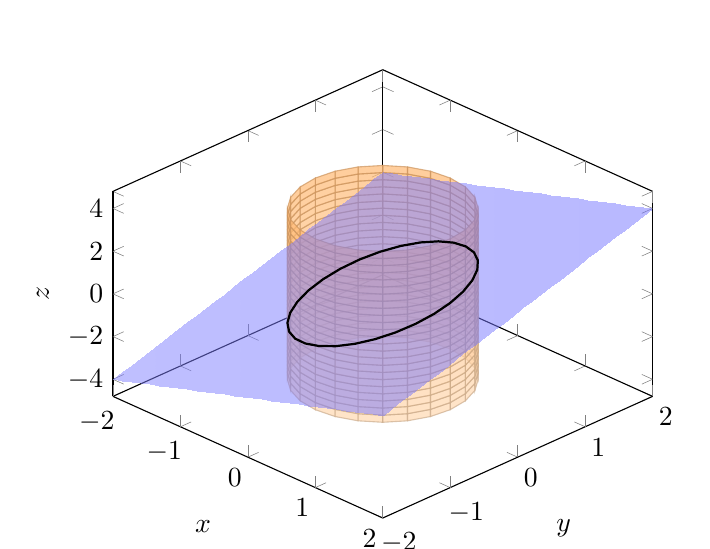
\begin{tikzpicture}
        \pgfdeclarelayer{pre main}
        \pgfsetlayers{pre main,main}
        
        \begin{axis}[
        view = {45}{40},
        xlabel = $x$,
        ylabel = $y$,
        zlabel = {$z$},
        ]
        
        \addplot3[surf,
        opacity=0.7,
        domain=0:360,
        y domain=-4:4, 
        colormap={mycol1}{color=(orange!30), color=(orange!55)}]
        ({cos(x)},{sin(x)},y);

        \addplot3[
        surf,
        colormap={mycol}{color=(blue!50), color=(blue!55)},
        samples=30,
        domain=-2:2,
        shader=interp,
        opacity=0.5,
        ]
        {x + y};
        

        \addplot3 [domain=0:360, samples=30, thick, colormap={mycol2}{color=(blue!30), color=(blue!30)}]
        ({cos(x)},{sin(x)}, {cos(x) + sin(x)});
        \end{axis}
    \end{tikzpicture}
    \caption{Graf iz zgleda \ref{zgl:10}}
\end{figure}

\begin{izrek}
    Naj bo $m < n$ in $D$ odprta podmnožica $\R^n$.
    Naj bo $G = (g_1, \dots, g_m) : D \to \R^m$ $C^1$ preslikava maksimalnega ranga $m$
    na $D$. Naj bo 
    $M = G^{-1} (\{0\}) \neq \emptyset$.
    Naj bo $f \in C^1 (D)$. Če ima $f$ v $p \in M$ lokalni ekstrem kot funkcija 
    $f: M \to \R$, obstajajo take konstante $\lambda_1, \dots, \lambda_m \in \R$, da je 
    $$(Df)(p) = \sum_{j = 1} ^m \lambda_j (Dg_j) (p).$$
\end{izrek}

    Konstante $\lambda_1, \dots, \lambda_m$ imenujemo tudi Lagrangevi multiplikatorji
    (množitelji). 
Izrek nam ponuja tako imenovano Lagrangevo metodo iskanja vezanih ekstremov.
Tvorimo funkcijo $$F(x_1, \dots, x_n, \lambda_1, \dots, \lambda_m) = f(x_1, \dots, x_n) - \sum_{1} ^m \lambda_j g_j (x_1, \dots, x_n)$$
in iščemo njene stacionarne točke. Tako moramo rešiti enačbe:
\begin{itemize}
    \item $\frac{\partial F}{\partial x_i} = \frac{\partial f}{\partial x_i} - \sum_1 ^m \lambda_j \frac{\partial g_j}{\partial x_i} = 0$ za $i \in \{1, \dots, n\}$,
    \item $\frac{\partial F}{\partial \lambda_j} =  - g_j = 0$ za $j \in \{1, \dots, m\}$.
\end{itemize}
Torej imamo $(n + m)$ enačb z $(n + m)$ neznankami.

\begin{dokaz}
   Naj ima $f \big| _M \to \R$ v točki $p \in M \subseteq D$ lokalni ekstrem.
   Trdimo, da je $(Df)(p)$ linearna kombinacija odvodov $(Dg_j)(p)$ za $j = 1, \dots, m$.
   Oglejmo si preslikavo $\Phi: D \to \R^{m + 1}$ s predpisom $x \mapsto (f(x), G(x))$, kjer je $m + 1 \leq n$.
   Odvod $\Phi$ v $p$ je enak 
   $$(D\Phi) (p) = \begin{bmatrix}
       Df\\ DG
   \end{bmatrix}(p).$$
   Če je rang te preslikave $m + 1$, je $\Phi$ surjektivna iz okolice $p$ v okolico $(f(p), 0)$.
   To pa pomeni, da obstajajo v tej okolici točke oblike $(f(p) - \varepsilon, 0)$ in $(f(p) + \varepsilon, 0)$
   za nek majhen $\varepsilon > 0$ in te točke so v sliki točk iz $M = G^{-1} (\{0\})$.
   Torej $f \big| _M$ v $p$ nima lokalnega ekstrema.
   Zato je $\rang G(p) = m$ (manj ne more biti) in od tod sledi, da je prva vrtica $(D \Phi) (p)$ 
   linearna kombinacija ostalih vrstic $(DG)(p)$.
\end{dokaz}

\begin{zgled}
    Naj bo $g_1 (x, y, z) = x^2 + y^2 + y^2 - 1$, $g_2 (x, y, z) = x + y + z$ in $f(x, y, z) = z$.
    Tvorimo funkcijo $F(x, y, z, \lambda, \mu) = z - \lambda (x^2 + y^2 + z^2 - 1) - \mu (x + y + z)$
    in dobimo sistem enačb:   
    \begin{itemize}
        \item $-2 \lambda x - \mu = 0$
        \item $-2 \lambda y - \mu = 0$
        \item $1 - 2 \lambda z - \mu = 0$
        \item $x^2 + y^2 + z^2 = 1$
        \item $x + y + z = 0$
    \end{itemize}
    Če ta sistem enačb rešimo, dobimo rešitev $\left(-\frac{\sqrt{6}}{6}, -\frac{\sqrt{6}}{6}, \frac{\sqrt{6}}{3}, \frac{\sqrt{6}}{6}, -\frac{1}{3}\right)$
    za maksimum in rešitev $\left(\frac{\sqrt{6}}{6}, \frac{\sqrt{6}}{6}, -\frac{\sqrt{6}}{3}, -\frac{\sqrt{6}}{6}, \frac{1}{3}\right)$
    za minimum.
\end{zgled}

\clearpage 
\section{INTEGRALI S PARAMETRI}

V tem poglevju bomo za različne funkcije opazovali integrale $F(y) = \int_a ^b f(x, y)\,dx$.

\begin{zgled}
    Definirajmo $F(y) = \int_0 ^\pi \sin (xy)\, dx$. S tem dobimo funkcijo 
    $$F(y) = \begin{cases}
        \frac{1 - \cos(\pi y)}{y} ;& y \neq 0\\
        0 ;& y = 0
    \end{cases}$$
\end{zgled}

\begin{zgled}\label{zgl:2}
    Eulerjeva funkcija gama, definirana kot $\Gamma (s) = \int_0 ^\infty x^{s - 1} e^{-x}\, dx$, je posplošeni integral.
    Integracijsko območje je neomejeno in za $s < 1$ je integrand neomejen v $0$, zato opazujemo 
    $$\Gamma (s) = \int_0 ^1 x^{s - 1} e^{-x}\, dx + \int_1 ^\infty x^{s - 1} e^{-x}\, dx.$$
    Drugi integral obstaja za vsak $s \in \R$, saj je $x^{s - 1} e^{-x} = \left(x^{s - 1} e^{-\frac{x}{2}}\right) e^{-\frac{x}{2}}$
    in $\lim_{x \to \infty} \left(x^{s - 1} e^{-\frac{x}{2}}\right) = 0$ in je torej to omejena funkcija.
    Prvi integral $\int_0 ^1 x^{s - 1} e^{-x}\, dx = \int_0 ^1 \frac{e^{-x}}{x^{1 - s}}\, dx$ pa obstaja natanko tedaj,
    ko je $1 - s < 1$ oziroma $s > 0$. Tako je definicijsko območje funkcije $\Gamma$ množica $D_\gamma = \{s \in \R,\ s > 0\}$.
    Sedaj vidimo, da je $\Gamma (1) = 1$. Z uporabo integracije per partes dobimo, da za vsak $s \in D_\Gamma$ velja 
    rekurzivna zveza $$\Gamma (s + 1) = s \Gamma (s).$$ Od tod pa sledi $\Gamma (n + 1) = n!$ za $n \in \N$. 
\end{zgled}

\begin{opomba}
    Pri evaluaciji Eulerjeve gama funkcije uporabimo osnovno rekurzivno zvezo $\Gamma (s + 1) = s \Gamma (s)$.
    Kasneje bomo pokazali, da je funkcija $\Gamma$ zvezna (oziroma celo gladka).
    Od tod sledi $$\lim_{s \downarrow 0} \Gamma (s) = \lim_{s \downarrow 0} \frac{\Gamma (s+1)}{s} = \lim_{s \downarrow 0} \frac{1}{s} = \infty,$$
    torej ima $\Gamma$ v točki $s = 0$ pol. Z zgornjo rekurzivno zvezo pa lahko $\Gamma$ razširimo tudi na množico 
    $\R \setminus \{0, -1, -2, \dots\}$.
\end{opomba}

\begin{figure}[htb!]
    \centering
    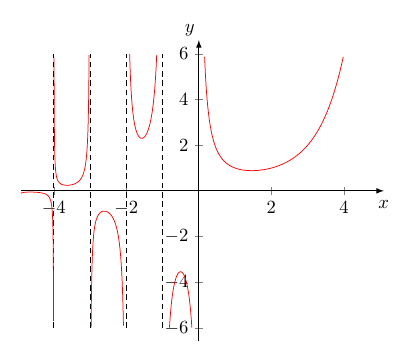
\includegraphics[scale=0.8]{gamafunkcija1.png}
    \caption{Funkcija $\Gamma$ iz zgleda \ref{zgl:2}.}
\end{figure}

\begin{zgled}
    Eulerjeva funkcija beta $B (p, q) = \int_0 ^1 x^{p - 1} (1 - x)^{q - 1}\, dx$.
    Kot pri gama funkciji ugotovimo, da je integral definiran za $p, q > 0$.
    Očitno pa je tudi, da velja $B(p, q) = B(q, p)$.
\end{zgled}

\subsection{Lastnosti integralov s parametri}

\begin{definicija}
    Podmnožica $Y \subseteq \R^n$ je lokalno kompaktna, če za $\forall y \in Y$ 
    obstaja okolica $\overline{K(y, r)}$, da je $Y \cap \overline{K(y, r)}$ kompaktna množica.
\end{definicija}

\begin{opomba}
    V prostoru $\R^n$ je ta lastnost ekvivalentna lokalni zaprtosti.
    Zvezne funkcije na lokalno kompaktnih množicah so lokalno omejene in lokalno enakomerno zvezne.
\end{opomba}

\begin{zgled}
    V $\R^n$ je tako vsaka odprta kot tudi vsaka zaprta podmnožica $\R^n$ lokalno kompaktna.
    Primer množice (v $\R^2$), ki pa ni lokalno kompaktna, je $Y = K(0, 1) \cup \{(1, 0)\}$.
\end{zgled}

\begin{izrek}[Zveznost integrala s parametri]\label{izr:1}
    Naj bo $I = [a, b]$ in $Y \subseteq \R^n$ lokalno kompaktna.
    Naj bo $f: I_x \times Y_y \to \R$ zvezna funkcija.
    Potem je $F: I_u \times I_v \times Y_y \to \R$ s predpisom 
    $$F(u, v, y) =\int_u ^v f(x, y)\, dx$$ zvezna na $I \times I \times Y$.
\end{izrek}

\begin{dokaz}
    Naj bo $(u_0, v_0, y_0) \in I \times I \times Y$.
    Dokazujemo zveznost $F$ v tej točki.
    Ker je $Y$ lokalno kompaktna, obstaja $r >0$, da je $Y \cap \overline{K(y_0, r)}$ kompaktna množica.
    Torej je tudi $I \times (Y \cap \overline{K(y_0, r)}) \subseteq \R^{n +1}$ kompaktna množica.
    Ker je $f: I \times Y \to \R$ zvezna, je na tej množici omejena, torej obstaja $0 < M < \infty$, da je 
    $|f(x, y)| \leq M$ za $\forall (x, y) \in I \times (Y \cap \overline{K(y_0, r)})$.

    Na tej množici pa je $f$ tudi enakomerno zvezna, torej za dani $\varepsilon > 0$
    obstaja tak $\delta > 0$, da za vsaka $y_1, y_2 \in Y \cap \overline{K(y_0, r)}$,
    ki ustrezata pogoju $|y_2 - y_1| < \delta,$ velja $|f(x, y_1) - f(x, y_2)| < \frac{\varepsilon}{3 (b - a)}$
    za vsak $x \in I = [a, b]$. Naj bosta sedaj $u, v \in I$ in $y \in Y \cap \overline{K(y_0, r)}$, da je 
    $|u - u_0| < \frac{\varepsilon}{3M}$, $|v - v_0| < \frac{\varepsilon}{3M}$ in $|y - y_0| < \delta$.
    Potem imamo 
    \begin{align*}
        |F(u, v, y) - F(u_0, v_0, y_0)| &= \left| \int_u ^v f(x, y)\, dx - \int_{u_0} ^{v_0} f(x, y_0)\, dx \right|\\
        &\leq \left| \int_u ^{u_0} f(x, y)\, dx \right| + \left| \int_{v_0} ^v f(x, y)\, dx \right| + \left| \int_{u_0} ^{v_0} (f(x, y) - f(x, y_0))\, dx \right|\\
        &< M|u - u_0| + M |v - v_0| + \frac{\varepsilon}{3(b - a)} \left| \int_{u_0} ^{v_0}\, dx \right| < \varepsilon,
    \end{align*}
    torej je $F$ zvezna v točki $(u_0, v_0, y)$ in posledično na $I \times I \times Y$.
\end{dokaz}

\begin{posledica}
    Naj bo $Y \subseteq \R^n$ lokalno kompaktna množica in $f: [a, b] \times Y \to \R$ zvezna funkcija.
    Tedaj je $F(y) = \int_a ^b f(x, y)\, dx$ zvezna na $Y$.
\end{posledica}

\begin{izrek}[Odvajanje integralov s parametri]
    Naj bodo $a < b$, $c < d$ in $f: [a, b] \times (c, d) \to \R$ zvezna.
    Za vsak $(x, y) \in [a, b] \times (c, d)$ naj obstaja parcialni odvod 
    $\frac{\partial f}{\partial y} (x, y) = f_y (x, y)$ in $f_y$ naj bo zvezna funkcija na $[a, b] \times (c, d)$.
    Tedaj je $F(y) = \int_a^b f(x, y)\, dx$ zvezno odvedljiva na $(c, d)$ in velja 
    $$\frac{d}{dy} \left(\int_a ^b f(x, y)\, dx \right) = \int_a ^b \frac{\partial f}{\partial y} (x, y)\, dx.$$
\end{izrek}

\begin{dokaz}
    Naj bo $y \in (c, d)$ in $[y - r, y + r] \subseteq (c, d)$ za nek $r > 0$.
    Naj bo $|h| < r$, $h \neq 0$ in $\varepsilon > 0$.
    \begin{align*}
        \left| \frac{F(y + h) - F(y)}{h} - \int_a ^b \frac{\partial f}{\partial y} (x, y)\, dx \right| &= 
        \left| \frac{1}{h} \int_a ^b (f(x, y + h) - f(x, y))\, dx -\int_a ^b \frac{\partial f}{\partial y} (x, y)\, dx \right| \\
        &= \left| \int_a ^b \left( \frac{\partial f}{\partial y} (x, y^*) - \frac{\partial f}{\partial y} (x, y) \right)\, dx \right|,
    \end{align*}
    kjer je $y^*$ med $y$ in $y + h$. Na $[a, b] \times [y - r, y + r]$ je $\frac{\partial f}{\partial y}$ enakomerno zvezna.
    Torej obstaja $\delta > 0$, da iz $y_1, y_2 \in [y - r, y + r]$, $|y_1 - y_2| < \delta$ sledi 
    $|f_y (x, y_1) - f_y (x, y_2) | < \frac{\varepsilon}{b - a}$ in to za vsak $x \in [a, b]$.
    Za tak $\delta > 0$ in $|h| < \delta$ velja $|y^* - y| < \delta$ in zato 
    \begin{equation*}
        \left| \frac{F(y + h) - F(y)}{h} - \int_a ^b f_y (x, y)\, dx \right| < \int_a ^b \frac{\varepsilon}{b - a}\, dx = \varepsilon. \qedhere
    \end{equation*}
\end{dokaz}

\begin{posledica}\label{pos:2}
    Naj bo $f$ kot v izreku in $\alpha, \beta: (c, d) \to [a, b]$ zvezno odvedljivi funkciji.
    Tedaj je funkcija $F(y) = \int_{\alpha(y)} ^{\beta(y)} f(x, y)\, dx$ zvezno odvedljiva na $(c, d)$ in velja 
    $$F'(y) = \int_{\alpha(y)} ^{\beta(y)} \frac{\partial f}{\partial y} (x, y)\, dx + \beta'(y) f(\beta(y), y) - \alpha'(y) f(\alpha (y), y).$$
\end{posledica}

\begin{dokaz}
    Definiramo $\Phi (u, v, y) = \int_u ^v f(x, y)\, dx$. Potem je $F(y) = \Phi (\alpha (y), \beta (y), y).$
    Vemo, da je $\frac{\partial \Phi}{\partial y} = \int_u ^v \frac{\partial f}{\partial y} (x, y)\, dx$,
    $\frac{\partial \Phi}{\partial v} = f(v, y)$ in $\frac{\partial \Phi}{\partial u} = -f(u, y)$.
    Sedaj pa po verižnemu pravilu dobimo 
    \begin{equation*}
        F'(y) = \Phi_y \cdot 1 + \Phi_u \cdot \alpha' + \Phi_v \cdot \beta'. \qedhere
    \end{equation*}
\end{dokaz}

\begin{posledica}
    Naj bo $D \subseteq \R^n$ odprta in $f: [a, b] \times D \to \R$ zvezna.
    Naj za vsak $(x, y) \in [a, b] \times D$ obstajajo parcialni odvodi $\frac{\partial f}{\partial y_j} (x, y) = f_{y_j} (x, y)$ za $j = 1, \dots, n$,
    ki so tudi zvezne funkcije na $[a, b] \times D$.
    Tedaj je $F(y) = \int_a ^b f(x, y)\, dx$ $C^1$ funkcija na $D$ in velja 
    $$\frac{\partial F}{\partial y_j} (y) = \int_a ^b \frac{\partial f}{\partial y_j} (x, y)\, dx$$
    za vsak $j = 1, \dots, n$.
\end{posledica}


\begin{zgled}
    Denimo, da želimo evaluirati integral $\int_0 ^1 \frac{dt}{(1 + t^2)^2}$.
    Vzemimo $F(a) = \int_0 ^1 \frac{dt}{t^2 + a^2}$ za $a > 0$.
    Od tod sledi $F'(a) = (-2a) \int_0 ^1 \frac{dt}{(t^2 + a^2)^2}$. Po drugi strani pa je 
    $F(a) = \frac{1}{a} \arctan \left(\frac{t}{a}\right) \Big|_0 ^1 = \frac{1}{a} \arctan \left(\frac{1}{a}\right)$.
    Tako imamo $\left(\frac{1}{a} \arctan \left(\frac{1}{a}\right)\right)' = - \frac{a + (a^2 + 1)\arctan \left(\frac{1}{a}\right)}{a^2 (a^2 + 1)}$
    in posledično
    $$\int_0 ^1 \frac{dt}{(t^2 + a^2)^2} = \frac{1 + \frac{(a^2 + 1)}{a}\arctan \left(\frac{1}{a}\right)}{2a^2 (a^2 + 1)}.$$
    Torej je $\int_0 ^1 \frac{dt}{(1 + t^2)^2} = \frac{2 + \pi}{8}$.
\end{zgled}

\begin{zgled}
    Vemo, da je $\int_0 ^a \frac{dx}{x^2 + a^2} = \frac{\pi}{4a}$. Če obe strani enačbe odvajamo s pomočjo posledice \ref{pos:2},
    dobimo 
    $$(-2a) \int_0 ^a \frac{dx}{(x^2 + a^2)^2} + \frac{1}{2a^2} = - \frac{\pi}{4a^2}$$ in od tod sledi 
    $\int_0 ^a \frac{dx}{(x^2 + a^2)^2} = \frac{2 + \pi}{8 a^3}$.
\end{zgled}

\begin{zgled}
    Naredimo podobno še za $\int_0 ^1 \frac{x - 1}{\ln x}\, dx$.
    Oglejmo si integral $F(a) = \int_0 ^1 \frac{x^a - 1}{\ln x}\, dx$ za $a \geq 0$.
    Z uporabo L'Hôpitalovega izreka pokažemo, da je funkcija $f(x, a) = \frac{x^a - 1}{\ln x}$ zvezna na $[0, 1] \times [0, \infty)$.
    Odvod zgornjega integrala je po izreku $F'(a) = \int_0 ^1 \frac{x^a \ln x}{\ln x}\, dx = \int_0 ^1 x^a\, dx$,
    saj je tudi $\frac{\partial f}{\partial a} (x, a) = x^a$ zvezna na $[0, 1] \times [0, \infty)$.
    Zato je $F'(a) = \frac{1}{a + 1}$. Od tod sledi $$F(a) = \ln (a + 1) + C$$ in ker je $F(0) = 0$, je tudi $C = 0$.
    Tako dobimo $\int_0 ^1 \frac{x - 1}{\ln x}\, dx = F(1) = \ln 2$.
\end{zgled}

\begin{izrek}[Integriranje integralov s parametri]
    Naj bo $f: [a, b]_x \times [c, d]_y \to \R$ zvezna.
    Tedaj je $$\int_c ^d \left( \int_a ^b f(x, y)\, dx \right)\, dy = \int_a ^b \left(\int_c ^d f(x, y)\, dy\right)\, dx.$$
\end{izrek}

\begin{dokaz}
    Naj bosta $\Phi(y) = \int_c ^y \left(\int_a ^b f(x, s)\, dx\right)\, ds$
    in $\Psi (y) = \int_a ^b \left(\int_c ^y f(x, s)\, ds\right)\, dx$.
    Dokazujemo $\Phi (d) = \Psi (d)$. Dokazali bomo, da za vsak $y \in [c, d]$ velja $\Phi(y) = \Psi (y)$.
    Očitno je $\Phi (y) = \Psi(c) = 0$. Dovolj je, da pokažemo še $\Phi'(y) = \Psi'(y)$ za $\forall y \in (c, d)$.

    Poglejmo odvoda. $\Phi'(y) = \frac{d}{dy} \left(\int_c ^y \left(\int_a ^b f(x, s)\, dx\right)\, ds \right) = \frac{d}{dy} \left(\int_c ^y F(s)\, ds\right)$.
    Po izreku \ref{izr:1} je $F(s)$ zvezna funkcija na $[c, d]$. Zato je po osnovnem izreku analize 
    funkcija $y \mapsto \int_c ^y F(s)\, ds$ odvedljiva in velja, da je njen odvod $\Phi'(y) = F(y) = \int_a ^b f(x, y) \, dx$.

    Sedaj si oglejmo še odvod $\Psi'(y) = \frac{d}{dy} \left(\int_a ^b \left(\int_c ^y f(x, s)\, ds\right)\, dx\right)$.
    Po izreku \ref{izr:1} je funkcija $(x, y) \mapsto \int_c ^y f(x, s)\, ds$ zvezna na $[a, b] \times [c, d]$
    in njen parcialni odvod po $y$ je $f(x,y)$, ki je tudi zvezna na $[a, b] \times [c, d]$, zato je $\Psi'(y) = \int_a ^b \frac{\partial}{\partial y} \left(\int_c ^y f(x, s) \, ds\right)\, dx = \int_a ^b f(x,y)\, dx$. 
\end{dokaz}

\subsection{Posplošeni integrali s parametrom}

\begin{definicija}
    Naj bo $Y$ dana množica in $f: [a, \infty) \times Y \to \R$ taka funkcija, da je za vsak $y \in Y$
    funkcija $x \mapsto f(x, y)$ zvezna na $[a, \infty)$. Naj za vsak $y \in Y$ 
    obstaja integral 
    $$F(y) = \int_a ^\infty f(x, y)\, dx = \lim_{b \to \infty} \int_a ^b f(x, y)\, dx.$$
    Ta integral je enakomerno konvergenten na $Y$, če za vsak $\varepsilon > 0$ obstaja tak $b_0 \geq a$,
    da za vsak $b \geq b_0$ in $y \in Y$ velja $\left| \int_b ^\infty f(x, y)\, dx \right| < \varepsilon$.
\end{definicija}

\begin{opomba}
    Če za vsak $ b \geq a$ definiramo $F_b (y) = \int_a ^b f(x, y) \, dx$,
    potem je pogoj iz definicije ekvivalenten pogoju, da $\lim_{b \to \infty} F_b (y) = F(y)$
    konvergira enakomerno na $Y$.
\end{opomba}

\begin{zgled}
    Vzemimo funkcijo $F(y) = \int_0 ^\infty y e^{-xy}\, dx$, kjer je $y \geq 0$.
    Potem je $F(0) = 0$ in za $y > 0$ dobimo $F(y) = -e^{-xy} \big|_0 ^\infty = 1$.
    Naj bo $c > 0$ in naj bo $Y = [c, \infty).$
    Potem imamo $\left| \int_b ^\infty y e^{-xy}\, dx \right| = e^{-by} \leq e^{-bc}$ za $y \geq c$ in $b \geq 0$.
    Potem obstaja tak $b_0$, da za $b \geq b_0$ velja $e^{-bc} \leq e^{-b_0 c} < \epsilon$,
    torej integral $F(y) = \int_0 ^\infty y e^{-xy}\, dx$ konvergira enakomerno na $[c, \infty)$ za vsak $c > 0$.
    Izkaže pa se, da ne konvergira enakomerno na $[0, \infty]$.
\end{zgled}

\begin{trditev}[Zadostni pogoji za enakomerno konvergenco]
    Naj bo $Y$ dana množica in $f:[0, \infty) \times Y \to \R$
    funkcija, ki je za vsak $y \in Y$ zvezna na $[a, \infty)$ .
    Če obstaja taka zvezna funkcija $\phi: [a, \infty) \to [0, \infty)$, da je 
    \begin{itemize}
        \item $|f(x, y)| \leq \phi(x)$ za vsak $(x, y) \in [a, \infty) \times Y$.
        \item obstaja $\int_a ^\infty \phi(x)\,dx < \infty$.
    \end{itemize}
    Tedaj integral $\int_a ^\infty f(x, y)\, dx$ konvergira enakomerno na $Y$.
\end{trditev}

\begin{dokaz}
    Naj bo $\varepsilon > 0$. Obstaja $b_0$, da za $b \geq b_0$ velja $\int_b ^\infty \phi(x)\, dx < \varepsilon$.
    Torej je za vsak $y \in Y$ 
    $$\left| \int_b ^\infty f(x, y)\, dx \right| \leq \int_b ^\infty |f(x, y)|\, dx \leq \int_b ^\infty \phi(x)\, dx < \varepsilon$$
    in integral za $F(y)$ konvergira enakomerno na $Y$.
\end{dokaz}

\begin{opomba}
    Za lastnosti, ki so lokalne narave (zveznost, odvedljivost)
    je običajno dovolj pogoj lokalne enakomerne konvergence: 
    naj bo $Y \subseteq \R^n$ lokalno kompaktna množica.
    Integral $F(y) = \int_a ^\infty f(x, y)\, dx$ za $y \in Y$ konvergira 
    lokalno enakomerno na $Y$, če za vsak $y \in Y$ obstaja okolica $K(y, r)$, da integral konvergira enakomerno na $K(y, r) \cap Y$.
    Ta pogoj je pri lokalno kompaktnih množicah ekvivalenten pogoju, da za 
    vsako kompaktno podmnožico $K \subseteq Y$ integral konvergira enakomerno na $K$.
\end{opomba}

\begin{zgled}
    Oglejmo si funkcijo $F(s) = \int_1 ^\infty x^{s - 1} e^{-x}\, dx$.
    Naj bo $M \geq 0$ in $s \in [-M, M]$.
    Tedaj je $x^{s - 1} e^{-x} \leq x^{M - 1} e^{-x}$, saj je $x \geq 1$. Ker 
    integral $\int_1 ^\infty x^{M - 1} e^{-x} \, dx$ obstaja, funkcija $F(s)$ konvergira enakomerno
    na $[-M, M]$ za vsak $M \geq 0$. Torej konvergira lokalno enakomerno na $\R$.
\end{zgled}

\begin{izrek}[Zveznost posplošenega integrala s parametrom]
    Naj bo $Y \subseteq \R^n$ lokalno kompaktna množica
    in naj bo $f: [a, \infty) \times Y \to \R$ zvezna. Če integral 
    $F(y) = \int_a ^\infty f(x, y)\, dx$ konvergira lokalno enakomerno na $Y$, je $F(y)$
    zvezna funkcija na $Y$.
\end{izrek}

\begin{dokaz}
    Naj bo $y_0 \in Y$ in $r > 0$, da je integral enakomerno konvergenten na $K(y_0, r)$.
    Vemo, da je za vsak $b \geq a$ integral $F_b (x) = \int_a ^b f(x, y)\, dx$ zvezna funkcija na $Y$ 
    in te funkcije konvergirajo enakomerno na $K(y_0, r)$ k $F$.
    Torej je $F$ zvezna na $K(y_0, r)$ in potemtakem zvezna na $Y$.
\end{dokaz}

\begin{zgled}
    Funkcija $\Gamma$ je zvezna na $(0, \infty)$, saj integral $s \mapsto \int_1 ^\infty x^{s - 1} e^{-x}\, dx$
    konvergira lokalno enakomerno na $\R$, integral $s \mapsto \int_0 ^1 x^{s - 1} e^{-x}\, dx$ pa je za $s > 0$
    le običajen integral zvezne funkcije v drugi obliki. Naj bo $0 < c \leq s$ in $n \in \N$ tak, da je 
    $ns - 1 \geq nc - 1 \geq 0$. Potem lahko vstavimo $x = t^n$ v integral in dobimo $n \int_0 ^1 t^{sn - 1} e^{-t^n}\, dt$.
    Ker je $t^{sn - 1} e^{-t^n}$ zvezna funkcija na $[0, 1] \times [c, \infty)$, je za $s_0 > 0$ funkcija 
    $s \mapsto \int_0 ^1 x^{s - 1} e^{-x}\, dx$ zvezna v $s_0$. Torej je $\Gamma$ zvezna na $(0, \infty)$.
\end{zgled}

\begin{izrek}[Integral posplošenega integrala s parametrom, Fubini]
    Naj bo $f: [a, \infty) \times [c, d] \to \R$ zvezna. Naj bo integral
    $F(y) = \int_a ^\infty f(x, y)\, dx$ enakomerno konvergenten na $[c, d]$.
    Tedaj je $$\int_c ^d \left(\int_a ^\infty f(x, y)\, dx\right)\, dy = \int_a ^\infty \left(\int_c ^d f(x, y)\, dy\right)\, dx.$$
\end{izrek}

\begin{dokaz}
    Funkcija $F(y)$ je zvezna funkcija na intervalu $[c, d]$, zato njen integral obstaja.
    Vemo, da je $\lim_{b \to \infty} F_b (y) = F(y)$ enakomerno na $[c, d]$.
    Zato po izreku iz analize 1 velja
    \begin{align*}
        \int_c ^d F(y)\, dy &= \lim_{b \to \infty} \int_c ^d F_b (y)\, dy\\
        &= \lim_{b \to\infty} \int_c ^d \left(\int_a ^b f(x, y)\, dx\right)\, dy\\
        &= \lim_{b \to \infty} \int_a ^b \left(\int_c ^d f(x, y)\,dy\right)\, dx\\
        &= \int_a ^\infty \left(\int_c ^d f(x, y)\, dy\right)\, dx \qedhere
    \end{align*}
\end{dokaz}

\begin{izrek}[Fubini]
    Naj bo $f: [a, \infty) \times [c, \infty) \to [0, \infty)$ zvezna in naj integrala 
    $F(y) = \int_a ^\infty f(x, y) \, dx$ in $G(x) = \int_c ^\infty f(x, y)\, dy$ konvergirata 
    lokalno enakomerno na $[c, \infty)$ oziroma $[a, \infty)$. Če obstaja 
    $\int_c ^\infty F(y)\, dy$, obstaja tudi $\int_a ^\infty G(x)\, dx$ in velja 
    $$\int_c ^\infty \left(\int_a ^\infty f(x, y)\, dx\right)\, dy = \int_a ^\infty \left(\int_c ^\infty f(x, y)\, dy\right)\, dx.$$
\end{izrek}

\begin{dokaz}
    Ker je $G(x)$ lokalno enakomerno konvergentna na (lokalno kompaktni) množici $[a, \infty)$,
    je enakomerno konvergentna na integralu $[a, b]$. Torej lahko uporabimo prejšnji izrek in dobimo 
    \begin{align*}
        \int_a ^b G(x)\, dx &= \int_a ^b \left(\int_c ^\infty f(x, y)\, dy\right)\, dx\\
        &= \int_c ^\infty \left(\int_a ^b f(x, y)\, dx\right)\, dy\\
        &\leq \int_c ^\infty \left(\int_a ^\infty f(x, y)\, dx\right)\, dy,
    \end{align*}
    torej obstaja $\int_a ^\infty G(x) \leq \int_c^\infty F(y)\, dy < \infty$.
    Sedaj lahko zamenjamo vlogi $F$ in $G$ in dobimo enakost.
\end{dokaz}

\begin{izrek}[Fubini]
    Naj bo $f: [a, \infty) \times [c, \infty) \to \R$ zvezna. Denimo, da je $y \mapsto \int_a ^\infty | f(x, y) |\, dx$
    lokalno enakomerno konvergentna na $[c, \infty)$ in 
    $x \mapsto \int_c ^\infty | f(x, y) |\, dx$
    lokalno enakomerno konvergentna na $[a, \infty)$.
    Če obstaja 
    $\int_c ^\infty \left(\int_a ^\infty |f(x, y)|\, dx\right) \, dy$, obstaja tudi $\int_a ^\infty \left(\int_c ^\infty |f(x, y)|\, dy\right) \, dx$ in sta enaka. Tedaj velja 
    $$\int_c ^\infty \left(\int_a ^\infty f(x, y)\, dx\right) \, dy = \int_a ^\infty \left(\int_c ^\infty f(x, y)\, dy\right) \, dx.$$
\end{izrek}

\begin{dokaz}
    Ker je $\left| \int_b ^\infty f(x, y)\, dx \right| \leq \int_b ^\infty | f(x, y) |\, dx$,
    integral $F(y) = \int_a ^\infty f(x, y)\, dx$ konvergira lokalno enakomerno na $[c, \infty)$
    in podobno $G(x) = \int_c ^\infty f(x, y)\, dy$ na $[a, \infty)$.
    Torej je $F$ zvezna na $[c, \infty)$ in $G$ na $[a, \infty)$.
    Prav tako je 
    \begin{align*}
        \int_a ^b G(x)\, dx &= \int_a ^b \left(\int_c ^\infty f(x, y)\, dy\right)\, dx\\
        &= \int_c ^\infty \left(\int_a ^b f(x, y)\, dx\right)\, dy\\
        &= \int_c ^\infty F_b (y)\, dy.
    \end{align*}
    Pokazati želimo, da je $\lim_{b \to \infty} \int_c ^\infty F_b (x) \, dx = \int_c ^\infty F(x)\, dx$.
    Naj bo $\varepsilon > 0.$ Po predpostavki je $\int_c ^\infty \left(\int_a ^\infty |f(x, y)|\, dx\right)\, dy < \infty$,
    zato obstaja tak $d \geq c$, da je 
    $$\left| \int_d ^\infty F(y)\, dy \right| \leq \int_d ^\infty \left(\int_a ^\infty |f(x, y)|\, dx\right)\, dy < \frac{\varepsilon}{3}.$$
    Poleg tega je $$\left| \int_d ^\infty F_b (y)\, dy \right| \leq \int_d ^\infty \left(\int_a ^b |f(x, y)|\, dx\right)\, dy \leq \int_d ^\infty \left(\int_a ^\infty |f(x, y)|\, dx\right)\, dy < \frac{\varepsilon}{3}.$$
    Ker tudi velja $\lim_{b \to \infty} \int_c ^d F_b(y)\, dy = \int_c ^d F(y) \, dy$, je za $b \geq b_0$
    $\left| \int_c ^d F_b(y)\, dy - \int_c ^d F(y) \, dy \right| < \frac{\varepsilon}{3}$.
    Torej za $b \geq b_0$ velja $\left| \int_c ^\infty F(y)\, dy - \int_c ^\infty F(y) \, dy \right| < \varepsilon$ in izrek je dokazan.
\end{dokaz}

\begin{izrek}[Odvedljivost posplošenega integrala s parametrom]
    Naj bo $f: [a, \infty) \times (c, d) \to \R$ zvezna.
    Naj bo v vsaki točki parcialno odvedljiva na $y$ in naj bo $f_y$ zvezna na 
    $[a, \infty) \times (c, d)$.
    Naj za $y \in (c, d)$ obstaja $F(y) = \int_a ^\infty f(x, y)\, dx$ in naj
    $y \mapsto \int_a ^\infty \frac{\partial f}{\partial y} (x, y)\, dx$ konvergira lokalno 
    enakomerno na $(c, d)$. Tedaj je $F$ zvezno odvedljiva na $(c, d)$ in velja 
    $$F'(y) = \int_a ^\infty \frac{\partial f}{\partial y} (x, y)\, dx.$$
\end{izrek}

\begin{dokaz}
    Naj bo $G(y) = \int_a ^\infty \frac{\partial f}{\partial y} (x, y)\, dx$. 
    Vemo, da je $G$ zvezna na $(c, d)$, saj je integral lokalno enakomerno konvergenten 
    na $(c, d)$. Naj bo $y_0 \in (c, d)$ in naj bo $\Phi (y) = \int_{y_0} ^y G(t)\, dt$
    za $y \in (c, d')$. Tedaj vemo, da je $\Phi$ odvedljiva na $(c, d)$ in $\Phi'(y) = G(y)$.
    Po drugi strani pa je 
    \begin{align*}
        \Phi (y) = \int_{y_0} ^y G(t)\, dt &= \int_{y_0} ^y \left(\int_a ^\infty \frac{\partial f}{\partial y}(x, t)\, dx\right)\, dt\\
        &= \int_a ^\infty \left(\int_{y_0} ^y \frac{\partial f}{\partial y}(x, t)\, dt\right)\, dx\\
        &= \int_a ^\infty f(x, y)\, dx - \int_a ^\infty f(x, y_0)\, dx\\
        &= F(y) - F(y_0),
    \end{align*}
    kar pomeni, da je $F$ odvedljiva in $F'(y) = \Phi'(y) = G(y).$
\end{dokaz} 

\begin{posledica}
    Naj bo $D \subseteq \R^n$ odprta in naj bo $f: [a, \infty) \times D \to \R$ zvezna.
    Naj obstajajo parcialni odvodi $\frac{\partial f}{\partial y_j} \in C([a, \infty) \times D)$ 
    za $j = 1, \dots, n$. Če integral $F(y) = \int_a ^\infty f(x, y)\, dx$ konvergira za $y \in D$
    in če integrali $G_j (y) = \int_a ^\infty \frac{\partial f}{\partial y_j} (x, y)\, dx$ 
    konvergirajo lokalno enakomerno na $D$, je $F$ $C^1$ funkcija na $D$ in velja 
    $$\frac{\partial F}{\partial y_j} (x) = \int_a ^\infty \frac{\partial f}{\partial y_j} (x, y)\, dx.$$
\end{posledica}

\begin{zgled}
    Izračunali bomo integral $\int_0 ^\infty \frac{\sin x}{x} \, dx = \frac{\pi}{2}$ s pomočjo integrala s parametrom.
    Definiramo $F(a) = \int_0 ^\infty e^{-ax} \frac{\sin x}{x}\, dx$ za $a \geq 0$ in iščemo $F(0)$.
    Najprej moramo pokazati, da integral $F(a)$ konvergira enakomerno na $[0, \infty)$ in je zato $F$ zvezna na $[0, \infty)$.
    Spomnimo se izreka iz analize 1, ki pravi, da za zvezno funkcijo $f: [\alpha, \beta] \to \R$ 
    in padajočo $C^1$ funkcijo $g: [\alpha, \beta] \to [0, \infty]$ obstaja $\gamma \in [\alpha, \beta]$,
    da je $\int_\alpha ^\beta f(x)g(x)\, dx = g(\alpha) \int_\alpha ^\gamma f(x)\, dx$.
    Uporabimo to trditev za $f(x) = \sin x$ in $g(x) = \frac{e^{-ax}}{x}$ in dobimo 
    $$\int_\alpha ^\beta \frac{e^{-ax}}{x} \sin x \, dx = \frac{e^{-a\alpha}}{\alpha} \int_\alpha ^\gamma \sin x \, dx = \frac{e^{-a\alpha}}{\alpha}  (- \cos x \big|_\alpha ^\beta).$$
    Torej je $\left| \int_\alpha ^\beta \frac{e^{-ax}}{x} \sin x \, dx \right| \leq \frac{e^{-a\alpha}}{\alpha} \cdot 2 \leq \frac{2}{\alpha}$ za $a \geq 0$.
    Torej vsi integrali $F(a)$ obstajajo za $a \geq 0$ in $F(a)$ je enakomerno konvergenten na $[0, \infty)$.
    Oglejmo si odvod. Kandidat je $F'(a) = - \int_0 ^\infty e^{-ax} \sin x \, dx$, ki za $c > 0$
    integral enekomerno konvergira na $[c, \infty)$ (a ne na $(0, \infty)$!), saj za $x \geq 0$ velja
    $\left| e^{-ax} \sin x \right| \leq e^{-cx}$ in $e^{-cx}$ je integrabilna na $[0, \infty)$, torej je 
    $F$ res odvedljiva na $(0, \infty)$. Sedaj poračunamo:
    \begin{align*}
        F'(a) &= - \int_0 ^\infty e^{-ax} \sin x \, dx\\
        &= - \int_0 ^\infty e^{-ax} \frac{e^{ix} - e^{-ix}}{2i} \, dx\\
        &= - \frac{1}{2i} \int_0 ^\infty \left(e^{-x(a-i)} - e^{-x(a+i)}\right) \, dx\\
        &= - \frac{1}{2i} \left(\frac{-1}{a - i} e^{-x(a-i)} - \frac{-1}{a + i} e^{-x(a+i)}\right) \Big|_0 ^\infty\\
        &= - \frac{1}{a^2 + 1}
    \end{align*} 
    in dobimo $F'(a) = -\frac{1}{a^2 + 1}$ in posledično $F(a) = - \arctan a + C$.
    Ker je $\lim_{a \to \infty} F(a) = 0$, je $C = \frac{\pi}{2}$ in $F(a) = - \arctan a + \frac{\pi}{2}$,
    zato je $F(0) = \frac{\pi}{2}$.
\end{zgled}

\begin{opomba}
    V integral $\int_0 ^\infty \frac{\sin (ax)}{x}\, dx$ za $a > 0$ vstavimo $ax = t$ in dobimo 
    $\int_0 ^\infty a \frac{\sin t}{t} \frac{dt}{a}\, dx = \frac{\pi}{2}$. Podobno naredimo še za $a < 0$ in dobimo 
    $\frac{2}{\pi} \int_0 ^\infty \frac{\sin (ax)}{x}\, dx = sgn (a)$.
\end{opomba}

\subsubsection{Eulerjevi funkciji gama in beta}

O Eulerjevi funkciji $\Gamma (s) = \int_0 ^\infty x^{s - 1} e^{-x}\, dx$
smo že povedali nekaj lastnosti, kot na primer dejstvo, da je zvezna na $(0, \infty)$,
zavzame vrednosti $\Gamma (1) = \Gamma(2) = 1$, zanjo velja rekurzivna relacija $\Gamma(s + 1) = s \Gamma(s)$
in $\Gamma(n + 1) = n!$ za $n \in \N$. Seveda pa si lahko ogledamo še njene odvode.
Ker integrali oblike $\int_0 ^\infty x^{s - 1} (\ln x)^n e^{-x}\, dx$
konvergirajo lokalno enakomerno na $(0, \infty)$, pa je 
funkcija $\Gamma$ tudi gladka na $(0, \infty)$ in velja 
$$\Gamma^{(k)} (s) = \int_0 ^\infty x^{s - 1} (\ln x)^k e^{-x}\, dx.$$
Od tod pa direktno sledi, da je $\Gamma$ konveksna na $(0, \infty)$,
saj $\Gamma^n > 0$ na $(0, \infty)$. O konveksnosti pa lahko povemo še več:
na enačbi $$\Gamma \left(\frac{s_1 + s_2}{2}\right) = \int_0 ^\infty \left(x^\frac{s_1 - 1}{2} e^{-\frac{x}{2}}\right) \left(x^\frac{s_2 - 1}{2} e^{-\frac{x}{2}}\right)\, dx$$
uporabimo Cauchy-Schwatzevo neenakost in dobimo 
$\Gamma \left(\frac{s_1 + s_2}{2}\right) \leq \sqrt{\Gamma(s_1)} \sqrt{\Gamma(s_2)}$,
zato je $$\ln \left(\frac{s_1 + s_2}{2}\right) \leq \frac{\ln \Gamma(s_1) + \ln \Gamma(s_2)}{2},$$
kar implicira (v kombinaciji z zveznostjo), da je funkcija $\ln \Gamma(s)$ konveksna.

\begin{opomba}
    Preverjanja konveksnosti zvezne funkcije $f: I \to \R$ z lastnostjo $f\left(\frac{x + y}{2}\right) \leq \frac{f(x) + f(y)}{2}$ bi se lotili z dokazovanjem
    zveze $$f \left(\frac{x_1 + \dots + x_k}{k}\right) \leq \frac{f(x_1) + \dots + f(x_k)}{k}$$ za poljuben $k \in \N$
    in vsak izbor $x_1, \dots, x_n \in I$. Ta neenakost velja za $k = 2^n$ po indukciji,
    izkaže pa se, da lahko tudi splošen primer $2^{n - 1} < k \leq 2^n$ prevedemo na prejšnjega s trikom:
    \begin{align*}
        f(\overline{x}) &= f \left(\frac{x_1 + \dots + x_k + (2^n - k)\overline{x}}{2^n}\right)\\
        &\leq \frac{f(x_1) + \dots + f(x_k) + (2^n - k)f(\overline{x})}{2^n}
    \end{align*}
\end{opomba}

\begin{opomba}
    Če je $\ln f$ konveksna, je tudi $f$ konveksna.
    Res, naj bo $f = e^h$, kjer je $h$ konveksna.
    Tedaj je $$f\left(\frac{x+y}{2}\right) = e^{h\left(\frac{x+y}{2}\right)} \leq e^{\frac{h(x)}{2}} e^{\frac{h(y)}{2}} = \sqrt{f(x)f(y)} \leq \frac{1}{2} (f(x) + f(y)).$$ 
\end{opomba}

\begin{opomba}
    Funkcija $\Gamma$ je enolično določena z lastnostmi:
    \begin{itemize}
        \item $\Gamma(1) = 1$
        \item $\Gamma(s + 1) = s \Gamma (s)$, $\forall s > 0$
        \item $\Gamma > 0$ je zvezna na $(0, \infty)$
        \item $\ln \Gamma$ je konveksna.
    \end{itemize}
\end{opomba}

\begin{zgled}
    Za $a > 0$ je 
    \begin{align*}
        \int_0 ^\infty e^{-ax^2}\, dx = \int_0 ^\infty \frac{1}{2 \sqrt{a}} t^{\frac{1}{2} - 1} e^{-t}\, dt = \frac{1}{2\sqrt{a}} \Gamma(\frac{1}{2}) = \frac{\sqrt{\pi}}{2 \sqrt{a}},
    \end{align*}
    kjer smo vstavili $t = ax^2$.
    Kasneje bomo dokazali, da je res $\Gamma(\frac{1}{2}) = \sqrt{\pi}$
\end{zgled}

\begin{zgled}
    V določeni integral funkcije Gaussove distribucije vpeljemo $u = x - a$
    in dobimo 
    \begin{align*}
        \int_{-\infty} ^\infty e^{-\frac{(x - a)^2}{2\sigma^2}} \, dx &= \int_{-\infty} ^\infty e^{-\frac{u^2}{2 \sigma^2}}\, du\\
        &= 2 \int_0 ^\infty e^{-\frac{u^2}{2\sigma^2}}\, du\\
        &= \sqrt{2 \pi} \sigma
    \end{align*}
    po prejšnjem zgledu.
    Torej je $\frac{1}{\sqrt{2\pi}\sigma} e^{-\frac{(x-a)^2}{2 \sigma^2}}$ gostota verjetnostne porazdelitve $N(a, \sigma)$,
    torej normalne porazdelitve s pričakovano vrednostjo $a$ in standardnim odklonom $\sigma$.
\end{zgled}

Funkcija gama je tesno povezana s funkcijo beta.
Spomnimo: $B(p, q) = B(q, p) = \int_0 ^1 x^{p - 1} (1 - x)^{q - 1}\, dx$ za $p, q > 0$.
Če vpeljemo $x = \sin^2 t$ in $1 - x = \cos^2 t$,
dobimo $B(p, q) = 2 \int_0 ^\frac{\pi}{2} \sin^{2p - 1} t \cos^{2q - 1} t\, dt$ 
in od tod $$\int_0 ^\frac{\pi}{2} \sin^\alpha t \cos^\beta t\, dt = \frac{1}{2} B\left(\frac{\alpha + 1}{2}, \frac{\beta + 1}{2}\right)$$
za $\alpha, \beta > -1$.

\begin{trditev}
    $B(p, q) = \int_0 ^\infty \frac{t^{p- 1}}{(1 + t)^{p + q}}\, dt$
\end{trditev}

\begin{dokaz}
    V $B(p, q) = \int_0 ^1 x^{p - 1}(1 - x)^{q - 1}\, dx$ vpeljemo $t = \frac{x}{1 - x}$ oziroma 
    $x = \frac{t}{1 + t}$ in $dx = \frac{dt}{(1 + t)^2}$. Tako je 
    \begin{equation*}
        B(p, q) = \int_0 ^\infty \frac{t^{p - 1}}{(1 + t)^{p - 1}} \frac{1}{(1 + t)^{q - 1}} \frac{dt}{(1 + t)^2} = \int_0 ^\infty \frac{t^{p- 1}}{(1 + t)^{p + q}}\, dt. \qedhere
    \end{equation*}
\end{dokaz}

\begin{posledica}
    $B(p, 1-p) = \int_0 ^\infty \frac{t^{p - 1}}{1 + t}\, dt$ za $0 < p < 1$.
\end{posledica}

\begin{posledica}
    $B(\frac{1}{2}, \frac{1}{2}) = \pi$.
\end{posledica}

\begin{dokaz}
    Vstavimo $t = x^2$ in dobimo $\int_0 ^\infty \frac{t^{-\frac{1}{2}}}{1 + t}\, dt = 2 \int_0 ^\infty \frac{dx}{1 + x^2} = 2 \arctan x \Big|_0 ^\infty = \pi$.
\end{dokaz}

\begin{opomba}
    Pri analizi 2b bomo dokazali $B(p, 1 - p) = \frac{\pi}{\sin (p \pi)}$ za $p \in (0, 1)$.
\end{opomba}

\begin{izrek}[Osnovna povezava med funkcijama beta in gama]
    $$B(p, q) = \frac{\Gamma(p) \Gamma(q)}{\Gamma(p+q)}$$
\end{izrek}

\begin{dokaz}
    \begin{align*}
        B(p, q) \Gamma(p + q) &= \left(\int_0 ^\infty \frac{t^{p - 1}}{(1 + t)^{p + q}}\, dt \right) \left(\int_0 ^\infty x^{p + q - 1} e^{-x}\, dx \right)\\
        &= \int_0 ^\infty \left(\int_0 ^\infty x^{p + q - 1} e^{-x}\, dx\right) \frac{t^{p - 1}}{(1 + t)^{p + q}}\, dt\\
        &= \int_0 ^\infty \left(\int_0 ^\infty \left(\frac{x}{1 + t}\right)^{p + q - 1} \frac{t^{p - 1}e^{-x}}{(1 + t)} \, dx\right) \, dt.\\
        \intertext{Najprej v notranji integral vpeljemo $\frac{x}{1 + t} = u$ in $dx = (1+ t) du$}
        &= \int_0 ^\infty \left(\int_0 ^\infty u^{p+q-1} t^{p-1} e^{-u} e^{-tu}\, du\right)\, dt\\
        &\stackrel{\text{Fubini}}{=} \int_0 ^\infty \left(\int_0 ^\infty u^{q-1} (ut)^{p-1} e^{-ut}e^{-u} u \, dt\right)\, du\\
        &= \int_0 ^\infty u^{q - 1} e^{-u} \left(\int_0 ^\infty (ut)^{p - 1} e^{-ut} u\, dt\right)\, du.\\
        \intertext{Sedaj v notranji integral vpeljemo še $ut = v$ in dobimo}
        &= \int_0 ^\infty u^{q - 1} e^{-u} \left(\int_0 ^\infty v^{p-1} e^{-v}\, dv\right)\, du\\
        &= \Gamma(p) \Gamma(q) \qedhere
    \end{align*}
\end{dokaz}

\begin{posledica}
    $\Gamma \left(\frac{1}{2}\right) = \sqrt{\pi}$
\end{posledica}

\begin{zgled}
    Uporabimo rezultate iz prejšnjih posledic na izračunu.
    \begin{itemize}
        \item $\Gamma \left(\frac{7}{2} \right) = \frac{5}{2} \frac{3}{2} \frac{1}{2} \Gamma \left(\frac{1}{2}\right) =\frac{35}{8} \sqrt{\pi}$
        \item $\int_0 ^\frac{\pi}{2} \sin^8 x \cos^6 x\, dx = \frac{1}{2} B\left(\frac{9}{2}, \frac{7}{2}\right) = \frac{\Gamma \left(\frac{9}{2}\right) \Gamma \left(\frac{7}{2}\right)}{2\Gamma(8)} = \frac{5\pi}{2^{12}}$
    \end{itemize}
\end{zgled}

\begin{izrek}[Stirlingova formula]
    $\lim_{s \to \infty} \frac{\Gamma(s + 1)}{s^s e^{-s} \sqrt{2 \pi s}} = 1$
\end{izrek}

\begin{dokaz}
    Po definiciji je $\Gamma (s + 1) = \int_0 ^\infty x^s e^{-x}\, dx$.
    Z odvodom dokažemo, da ima funkcija $x \mapsto x^s e^x$ maksimum v $x = s$, ki je enak $s^s e^{-s}$.
    Vpeljimo $x = (1 + u) s$, tako da bo maksimum v $u = 0$.
    Tedaj je 
    $$\Gamma (s + 1) = \int_{-1} ^\infty s^s (1 + u)^s e^{-s} e^{-su} s\, du = s^s e^{-s} s \int_{-1} ^\infty \left((1 + u)e^{-u}\right)^s \, du.$$
    Zanima nas limita $\lim_{s \to \infty} \frac{\Gamma(s + 1)}{s^s e^{-s} \sqrt{s}} = \lim_{s \to \infty} \sqrt{s} \int_{-1} ^\infty \left((1 + u) e^{-u}\right)^s\, du$.
    Funkcija $u \mapsto (1 + u) e^{-u}$ ima maksimum $1$ v točki $u = 0$.
    Na intervalu $(-1, 0)$ ta funkcija narašča, na $(0, \infty)$ pa pada.
    Za $|u| < 1$ si oglejmo $\ln ((1 + u) e^{-u}) = \ln(1 + u) - u = -\frac{u^2}{2} + u^3 \phi(u)$,
    kjer je $\phi(u) = \frac{1}{3} - \frac{u}{4} + \frac{u^2}{5} - \dots$
    Za vsak $u > -1$ lahko definiramo 
    $$\phi(u) = \frac{\ln((1 + u)e^{-u}) + \frac{u^2}{2}}{u^3},$$
    ki je gladka funkcija na $(-1, \infty)$. Torej je $(1 + u)e^{-u} = e^{-\frac{u^2}{2}} e^{u^3 \phi(u)}$ in 
    $\sqrt{s} \int_{-1} ^\infty \left((1 + u) e^{-u}\right)^s\, du = \sqrt{s} \int_{-1} ^\infty e^{-\frac{su^2}{2}} e^{su^3 \phi(u)} \, du$.
    Če vpeljemo $\sqrt{s} u = v$, dobimo $\int_{-\sqrt{s}} ^\infty e^{-\frac{v^2}{2}} e^{\frac{v^3}{\sqrt{s}} \phi\left(\frac{v}{\sqrt{s}}\right)}\, dv$.
    Opazimo $$\sqrt{s} \int_{1} ^\infty \left((1 + u) e^{-u}\right)^s\, du \leq 2^{s - 1} e^{-(s-1)} \sqrt{s} \int_{1} ^\infty (1 + u) e^{-u}\, du \leq M \sqrt{s} \left(\frac{2}{e}\right)^{s - 1},$$
    kar konvergira proti $0$, ko gre $s$ preko vsake meje. Tako je dovolj pokazati 
    $$\lim_{s \to \infty} \int_{-\sqrt{s}} ^{\sqrt{s}} e^{-\frac{v^2}{2}} e^{\frac{v^3}{\sqrt{s}} \phi\left(\frac{v}{\sqrt{s}}\right)} \, dv = 2 \pi.$$
    Ker je funkcija $u \mapsto (1 + u) e^{-u}$ taka, da od $-1$ do $0$ narašča in nato povsod pada,
    potem integrand $e^{-\frac{v^2}{2}} e^{\frac{v^3}{\sqrt{s}} \phi\left(\frac{v}{\sqrt{s}}\right)}$ narašča od $- \sqrt{s}$ do $0$ in nato pada.
    Pišimo $s = r^{10}$ in $s \to \infty$ natanko tedaj, ko $r \to \infty$.
    Integral razdelimo na tri dele:
    \begin{enumerate}
        \item $\int_{-r^5} ^r e^{-\frac{v^2}{2}} e^{\frac{v^3}{r^5} \phi\left(\frac{v}{r^5}\right)} \, dv$
        \item $\int_{-r} ^{r} e^{-\frac{v^2}{2}} e^{\frac{v^3}{r^5} \phi\left(\frac{v}{r^5}\right)} \, dv$
        \item $\int_r ^{r^5} e^{-\frac{v^2}{2}} e^{\frac{v^3}{r^5} \phi\left(\frac{v}{r^5}\right)} \, dv$.
    \end{enumerate}
    Vzemimo $r \geq 1$ in ocenimo integral $|I_1| \leq r^5 e^{-\frac{r^2}{2}} e^{\frac{1}{r^2} \phi \left(\frac{1}{r^4}\right)}$.
    Podobno lahko ocenimo tudi integral $|I_3| \leq r^5 e^{-\frac{r^2}{2}} e^{\frac{1}{r^2} \phi \left(\frac{1}{r^4}\right)}$ in
    ti dve oceni gresta proti $0$, ko gre $r \to \infty$.
    Ocenimo še drugi integral: funkcija $\phi$ je omejena v okolici $0$, zato 
    $$e^{-\frac{M}{r^2}} \int_{-r} ^r e^{-\frac{v^2}{2}}\, dv \leq I_2 \leq e^{\frac{M}{r^2}} \int_{-r} ^r e^{-\frac{v^2}{2}}\, dv$$
    in v limiti, ko gre $r$ preko vsake meje, dobimo $\lim_{r \to \infty} I_2 = \int_{-\infty} ^\infty e^{-\frac{v^2}{2}}\, dv = \sqrt{2\pi}$.
\end{dokaz}

\begin{posledica}
    $\lim_{n \to \infty} \frac{n!}{n^n e^{-n} \sqrt{2 \pi n}} = 1$
\end{posledica}

\begin{zgled}
    \begin{align*}
        \lim_{n \to \infty} \frac{(2n)!}{n!\, n^n\, 2^n} &= \lim_{n \to \infty} \frac{(2n)^{2n} e^{-2n} \sqrt{4 \pi n}}{n^n\, e^{-n}\, n^n\, 2^n\, \sqrt{2 \pi n}}\\
        &= \lim_{n \to \infty} \frac{2^n}{e^n} \sqrt{2}\\ 
        &= \lim_{n \to \infty} \sqrt{2}\, \left(\frac{2}{e}\right)^n = 0.
    \end{align*}
\end{zgled}
\clearpage
\section{RIEMANNOV INTEGRAL V $\R^n$}

Spomnimo se našega dogovora, da za $a = (a_1, \dots, a_n)$ in $b = (b_1, \dots, b_n)$
velja $a < b$ natanko tedaj, ko je $a_j < b_j$ za vse $j = 1, \dots, n$.
Potem je zaprt kvader množica oblike $[a, b] = \{x \in \R;\ a \leq x \leq b\}$.
Kvadri, ki jih obravnavamo, imajo vse svoje robove vzporedne koordinatnim osem, njihov volumen pa je 
$\prod_1 ^n (b_j - a_j)$.

Sedaj si oglejmo delitve kvadra.
Če vsako stranico $[a_j, b_j]$ za $j = 1, \dots, n$ razdelimo na 
$$a_j = x_0 ^{(j)} < x_1 ^{(j)} < \dots < x_{m_j} ^{(j)} = b_j,$$
kjer je $m_j \in \N$, potem kvader $K = [a, b]$ razdelimo na $m_1 \dots m_n$ kvadrov oblike 
$$[x_{e_1 - 1} ^{(1)}, x_{e_1}^{(1)}] \times \dots \times [x_{e_n - 1} ^{(n)}, x_{e_n}^{(n)}]$$
za $0 < e_j \leq m_j$. Delitev $D$ kvadra $K$ torek podajamo z delitvami stranic kvadra $K$.

\begin{definicija}
    Delitev $D'$ je finejša od delitve $D$ oziroma je njeno 
    nadaljevanje, če vsebuje vse delilne točke delitve $D$ in morda ša kakšno zraven.
\end{definicija}

\begin{opomba}
    Če je $D'$ finejša od $D$, je vsak kvader delitve $D'$ vsebovan 
    v nekem kvadru delitve $D$ in vsak kvader delitve $D$ je unija nekaj kvadrov iz $D'$.
    Če kvadri $K_1, \dots, K_N$ sestavljajo delitev kvadra $K$, velja $\sum_1 ^N V(K_j) = V(K)$.
\end{opomba}

Naj bo sedaj $F: K \to \R$ omejena funkcija in označimo $m(K) = \inf_K f$ in $M(K) = \sup_K f$.

\begin{definicija}
    Naj bo $D$ delitev $K$ s kvadri delitve $K_1, \dots, K_N$.
    Spodnja Darbouxjeva vsota $f$ pri delitvi $D$ je $s(f, D) = s(D) = \sum_1 ^N m(K_j) V(K_j)$,
    zgornja pa $S(f, D) = S(D) = \sum_1 ^N M(K_j) V(K_j).$
\end{definicija}

Očitno velja $m(K) V(K) \leq s(D) \leq S(D) \leq M(K) V(K)$.

\begin{trditev}
    Če je $D'$ finejša od $D$, je 
    $s(D) \leq s(D') \leq S(D') \leq S(D)$.
\end{trditev}

\begin{dokaz}
    Sledi po indukciji.
\end{dokaz}

\begin{posledica}
    Naj bosta $D_1, D_2$ delitvi $K$.
    Potem je $s(D_1) \leq S(D_2)$.
\end{posledica}

\begin{dokaz}
    Naj bo $D' = D_1 \cup D_2$. Potem je $s(D_1) \leq s(D') \leq S(D') \leq S(D_2)$.
\end{dokaz}

Sedaj definirajmo $s = \sup_D s(D)$ in $S = \inf_D S(D)$. Očitno je $s \leq S$.

\begin{definicija}
    Omejena funkcija $f: K \to \R$ je na $K$ po Darbouxju integrabilna, če je 
    $s = S = I_D$ in ta vrednost je Darbouxjev integral $f$ po $K$:
    $$\int_K f(x)\, dx = \int_K f(x)\, dV(x) = \int \dots \iint f(x_1, \dots, x_n) \, dx_1\, dx_2\, \dots\, dx_n.$$
\end{definicija}

Druga možna definicija je z Riemannovimi vsotami.
Za $f: K \to \R$, delitev $D$ kvadra $K$ in izbor točk $\xi = \{\xi_j;\ \xi_j \in K_j\}$,
kjer $K_j$ označuje kvadre delitve $D$, je $R(f, D, \xi) = \sum_j f(\xi_j) V(K_j)$
Riemannova vsota funkcije $f$ pri delitvi $D$ in izboru točk $\xi$.

\begin{definicija}
    Funkcija $f: K \to \R$ je na $K$ Riemannovo integrabilna, če je 
    $\lim_{\delta \to 0} R(f, D, \xi) = I_R$, t.j. za vsak $\varepsilon > 0$
    obstaja tak $\delta > 0$, da za vsako delitev $D$ kvadra $K$ s kvadri $K_1, \dots, K_N$,
    katerih vse stranice so krajše od $\delta$, velja $|R(f, D, \xi) - I_R|$ za poljuben izbor točk $\xi$.
    Vrednost limite $I_R$ je Riemannov integral $f$ po $K$.
\end{definicija}

\begin{zgled}
    Osnoven zgled funkcije, ki je tako po Darbouxju kot tudi po Riemannu integrabilna,
    je konstantna funkcija. Nasprotno pa je primer funkcije, ki ni integrabilna, funkcija 
    $$f(x, y) = \begin{cases}
        1 ;& x, y \in \Q\\
        0 ;& \textrm{sicer}
    \end{cases}$$
\end{zgled}

\begin{opomba}
    Kot pri analizi 1 se vidi, da obstoj Riemannovega integrala implicira, da je 
    $f$ omejena na $K$.
\end{opomba}

\begin{izrek}
    Naj bo $f: K \to \R$ omejena. Naslednje trditve so ekvivalentne.
    \begin{enumerate}
        \item Funkcija $f$ je integrabilna po Darbouxju.
        \item Funkcija $f$ je integrabilna po Riemannu.
        \item Za vsak $\varepsilon > 0$ obstaja taka delitev $D$ kvadra $K$, da je $S(D) - s(D) < \varepsilon$.
    \end{enumerate}
    Tedaj je vrednost Riemannovega integrala enaka Darbouxjevi.
\end{izrek}

\begin{lema}
    Naj bo $D_0$ delitev $K$.
    Za vsak $\varepsilon > 0$ obstaja tak $\delta > 0$, da za 
    vsako delitev $D$, katere vsi kvadri imajo vse stranice krajše od $\delta$,
    je skupna prostornina kvadrov $D$, ki niso v celoti vsebovani v kakšnem 
    od kvadrov delitve $D_0$, manjša od $\varepsilon$.
\end{lema}

\begin{dokaz}[Dokaz pomožne trditve]
    Za splošno dimenzijo prostora $n > 1$ to trditev dokažemo tako,
    da vzamemo vse notranje robne ploskve delitve $D_0$ (ki so ploskve
    dimenzije $n-1$) in jih "`odebelimo"' za $2 \delta$.
    Torej seštejemo volumen robnih ploskev, ga označimo s $T$ in definiramo $\delta =\frac{\varepsilon}{2T}$.
\end{dokaz}

\begin{dokaz}[Dokaz izreka]
    Dokažimo implikacijo $(1) \Rightarrow (2)$.
    Naj bo $s = S = I$. Naj bo $\varepsilon > 0$.
    Vemo, da je $f$ omejena, torej obstaja $0 < M \in \R$, da je $|f(x)| \leq M$ za $\forall x \in K$.
    Potem obstaja taka delitev $D_0$, da je 
    $$I - \frac{\varepsilon}{2} < s(D_0) \leq S(D_0) < I + \frac{\varepsilon}{2}.$$
    Zaradi pomožne trditve obstaja tak $\delta > 0$, da za vsako delitev $D$,
    katere vsi kvadri imajo vse stranice manjše od $\delta$, velja, da je vsota prostornin kvadrov,
    ki niso vsebovani v enem od kvadrov delitve $D_0$, manjša od $\frac{\varepsilon}{2 M}$.
    Naj bo $D$ taka delitev s kvadri $K_1, \dots, K_N$,
    kjer so $K_1, \dots, K_l$ vsebovani v kakšnem od kvadrov $D_0$, 
    $K_{l + 1}, \dots, K_N$ pa ne. Torej je $\left| \sum_{l + 1} ^N f(\xi_j) V(K_j) \right| < \frac{\varepsilon}{2}$.
    Če pa je $K_j \subseteq K_l ^{(0)}$, velja tudi $m(K_j) \geq m(K_l ^{(0)})$ in $M(K_j) \leq M(K_l ^{(0)})$.
    Potem je $$\sum_1 ^l f(\xi_j) V(K_j) \leq \sum_1 ^l m(K_j) V(K_j) \leq S(D_0)$$
    in podobno $$\sum_1 ^l f(\xi_j) V(K_j) \geq \sum_1 ^l m(K_j) V(K_j) \geq s(D_0).$$
    Torej je 
    \begin{align*}
        \left| R(f, D, \xi) - I_D \right| &\leq \left| \sum_1 ^l f(\xi_j) V(K_j) - I_D \right| + \left| \sum_{l + 1} ^N f(\xi_j) V(K_j) \right|\\
        &< \frac{\varepsilon}{2} + \frac{\varepsilon}{2} = \varepsilon \qedhere
    \end{align*}
\end{dokaz}

\begin{izrek}
    Naj bo $f: K \to \R$ zvezna. Potem je $f$ integrabilna na $K$. 
\end{izrek}

\begin{dokaz}
    Množica $K$ je kompaktna, torej je $f$ enakomerno zvezna na $K$.
    Naj bo $\varepsilon > 0$. Potem obstaja $\delta > 0$, da iz 
    $\max \{|x_1 - y_1|, \dots, |x_n - y_n|\} < \delta$ sledi $|f(x) - f(y)| < \frac{\varepsilon}{V(K)}$.
    Naj bo $D$ delitev s kvadri z robovi pod $\delta$:
    \begin{align*}
        S(D) - s(D) &= \sum_1 ^N (M(k_j) - m(k_j)) V(K_j)\\
        &= \sum_1 ^N (f(x_j) - f(y_j)) V(K_j)\\
        &< \frac{\varepsilon}{V(K)} V(K_j) = \varepsilon \qedhere
    \end{align*}
\end{dokaz}

\begin{trditev}[Lastnosti integrala po kvadrih]
    Naj bosta $f, g: K \to \R$ integrabilni in $\alpha \in \R$. 
    \begin{itemize}
        \item Funkcije $f \pm g$ in $\alpha f$ so integrabilne na $K$ in velja 
        $\int_K (f + g)(x)\, dx = \int_K f(x)\, dx + \int_K g(x)\, dx$ ter 
        $\int_K \alpha f(x)\, dx = \alpha \int_K f(x)\, dx$
        (integrabilne funkcije na $K$ torej tvorijo vektorski prostor nad $\R$ in integral je linearen funkconal na tem prostoru).
        \item Če je $f(x) \leq g(x)$ za vsak $x \in K$, je $\int_K f(x)\, dx \leq \int_K g(x)\, dx$.
        \item Funkcija $|f|$ je integrabilna na $K$ in $\left| \int_K f(x)\, dx \right| \leq \int_K |f(x)|\, dx$.
    \end{itemize}
\end{trditev}

\subsection{Lastnosti integrala}

\begin{izrek}[Fubini]
    Naj bosta $A \subseteq \R^n$, $B \subseteq \R^m$ kvadra. Naj bo $f: A_x \times B_y \to \R$ integrabilna.
    \begin{enumerate}
        \item Naj bo za vsak $x \in A$ integrabilna funkcija $f^x (y) = f(x, y)$ na $B$.
        Tedaj je funkcija $x \mapsto \int_B f(x, y)\, dy$ integrabilna na $A$ in velja 
        $$\iint_{A \times B} f(x, y)\, dx\, dy = \int_A \left(\int_B f(x, y)\, dy\right)\, dx.$$
        \item Naj bo za vsak $y \in B$ integrabilna funkcija $f^y (x) = f(x, y)$ na $A$.
        Tedaj je funkcija $y \mapsto \int_A f(x, y)\, dx$ integrabilna na $B$ in velja 
        $$\iint_{A \times B} f(x, y)\, dx\, dy = \int_B \left(\int_A f(x, y)\, dx\right)\, dy.$$
    \end{enumerate} 
\end{izrek}

\begin{posledica}
    Če je $f: A \times B \to \R$ zvezna, je 
    $$\iint_{A \times B} f(x, y)\, dx\, dy = \int_A \left(\int_B f(x, y)\, dy\right)\, dx. = \int_B \left(\int_A f(x, y)\, dx\right)\, dy.$$
\end{posledica}

\begin{posledica}
    Naj bo $f: [a, b] \times [c, d] \to \R$ zvezna. Potem je 
    $$\iint_{[a, b] \times [c, d]} f(x, y)\, dx\, dy = \int_a ^b \left(\int_c ^d f(x, y)\, dy\right)\, dx = \int_c ^d \left(\int_a ^b f(x, y)\, dx\right)\, dy.$$
\end{posledica}

\begin{posledica}
    Naj bo $f: [a, b] \times [c, d] \times [g, h] \to \R$ zvezna. Potem je 
    $$\iint_{[a, b] \times [c, d] \times [g, h]} f(x, y, z)\, dx\, dy\, dz = \int_a ^b \left(\int_c ^d \left(\int_g ^h f(x, y, z)\, dz\right)\, dy\right)\, dx$$
    in to je enako vsem ostalim permutacijam vrstnega reda integriranja.
\end{posledica}

\begin{dokaz}
    Dokažimo prvo točko. Naj bo $g(x) = \int_B f^x (y)\, dy = \int_B f(x, y)\, dy$.
    Naj bodo $A_1, \dots, A_N$ vse kvadri delitve $D_A$ in $B_1, \dots, B_M$ vsi kvadri 
    delitve $D_B$. Kvadri $K_{ij}$ torej tvorijo delitev $D_A \times D_B$ množice $A \times B$.
    Naj bo $m_{ij} = \inf_{K_{ij}} f$ in $M_{ij} = \sup_{K_{ij}} f$. Vzemimo $x \in A_i$, potem je 
    $m_{ij} \leq \inf_{B_j} f^x \leq \sup_{B_j} f^x \leq M_{ij}$.
    Torej je 
    $$\sum_j m_{ij} V(B_j) \leq s(f^x, D_B) \leq S(f^x, D_B) \leq \sum_j M_{ij} V(B_j)$$
    in zato $\sum_j m_{ij} V(B_j) \leq \int_B f^x (y)\, dy = g(x) \leq \sum_j M_{ij} V(B_j)$ za vsak $x \in A$.
    Od tod sledi $$\sum_j m_{ij} V(B_j) \leq \inf_{A_{i}} g \leq \sup_{A_{i}} g \leq \sum_j M_{ij} V(B_j)$$
    in zato $s(f, D_A \times D_B) \leq s (g, D_A) \leq S(g, D_A) \leq S(f, D_A \times D_B)$.
    Ker je $f$ integrabilna na $A \times B$, je tudi $g$ integrabilna na $A$ in velja 
    \begin{equation*}
        \iint_{A \times B} f(x, y)\, dx\, dy = \int_A \left(\int_B f(x, y)\, dy\right)\, dx. \qedhere
    \end{equation*} 
\end{dokaz}

\begin{zgled}\label{zgl:3}
    Naj bo $f(x, y) = 1 - \frac{1}{3}x - \frac{1}{4}y$ in $P = [0, 1] \times [0, 1]$.
    Potem je prostornina množice pod grafom $f$ na področju $P$ enaka 
    \begin{align*}
        V(T) = \iint_{[0, 1] \times [0, 1]}\left(1 - \frac{1}{3}x - \frac{1}{4}y\right)\, dx\, dy &= \int_0 ^1 \left(\int_0 ^1 \left(1 - \frac{1}{3}x - \frac{1}{4}y\right)\, dy\right)\, dx\\
        &= \int_0 ^1 \left(1 - \frac{1}{3}x - \frac{1}{8}y\right)\, dx\\
        &=\frac{17}{24}
    \end{align*}
\end{zgled}

\begin{figure}[htb!]
    \centering
    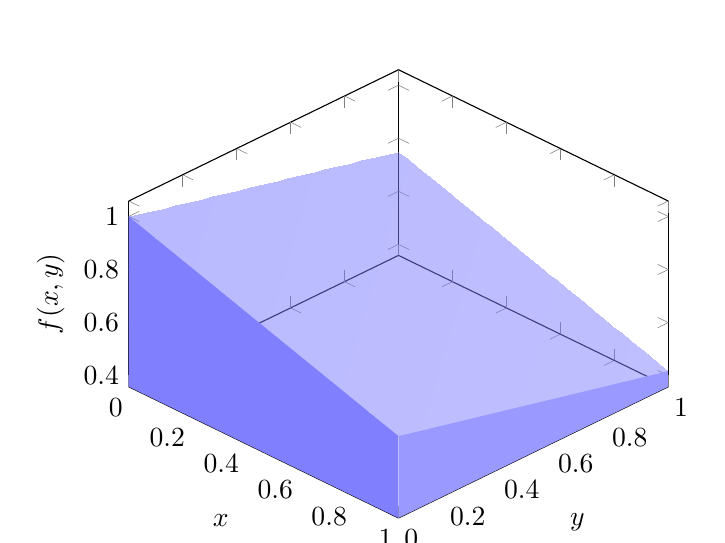
\begin{tikzpicture}[declare function={f(\x,\y)= 1 - (\x/3) - (\y/4);}]
        \pgfdeclarelayer{pre main}
        \pgfsetlayers{pre main,main}
        
        \begin{axis}[
        view = {45}{45},
        colormap={mycol}{color=(blue!50), color=(blue!55)},
        xlabel = $x$,
        ylabel = $y$,
        zlabel = {$f(x,y)$},
        ]
        
        \addplot3[
        surf,
        samples=30,
        domain=0:1,
        shader=interp,
        opacity=0.5,
        ]
        {f(x,y)};
        
        \fill[blue!50] (0,0,0) -- plot[variable=\x,domain=0:1] (\x,0,{f(\x,0)}) -- (1,0,0) --
        cycle;
        \fill[blue!40] (1,0,0) -- plot[variable=\y,domain=0:1] (1,\y,{f(1,\y)}) 
        -- (1,1,0) --cycle;
        
        \end{axis}
    \end{tikzpicture}
    \caption{Graf iz zgleda \ref{zgl:3}}
\end{figure}

Oglejmo si integral po poljubni neprazni omejeni množici $A$.
Naj bo $A$ omejena podmnožica $\R^n$. Naj bo $f: A \to \R$ omejena.
Funkcijo $f$ razširimo na $\R^n$ kot funkcijo $$\widetilde{f} (x) = \begin{cases}
    f(x) ;& x \in A\\
    0 ;& x \notin A
\end{cases}.$$
Lahko pa tudi vpeljemo karakteristično funkcijo $A$ kot 
$$\chi_A (x) = \begin{cases}
    1 ;& x \in A\\
    0 ;& x \notin A
\end{cases}$$
in potlej lahko pišemo $\widetilde{f} = f \cdot \chi_A$.
Naj bo $K$ kvader, ki vsebuje $A$, torej $A \subseteq K$.

\begin{definicija}
    Funkcija $f$ je integrabilna na množici $A$, če je $\widetilde{f}$ integrabilna na $K$.
    Tedaj definiramo $\int_A f(x)\, dx = \int_K \widetilde{f}(x)\, dx$.
\end{definicija}

\begin{opomba}
    Ta definicija je odvisna od izbora kvadra $K$, ki vsebuje $A$, vendar pa se izkaže, da 
    kvader ne vpliva na vrednost integrala $\widetilde{f}$.
\end{opomba}

\begin{zgled}
    Naj bo $A = \Q^2 \cap [0, 1]^2 \subseteq \R^2$ in $f: A \to \R$ s predpisom $f(x, y) = 1$.
    Torej je $A$ konstantna funkcija na $A$ in tako tudi zvezna na $A$, kljub temu pa integral $f$ po $A$ 
    ne obstaja, saj funkcija 
    $$\widetilde{f} (x, y) = \begin{cases}
        1 ;& (x, y) \in A\\
        0 ;& \mathrm{sicer}
    \end{cases}$$ ni integrabilna na $[0, 1]^2$.
    Torej je obstoj integrala $\int_A f(x)\, dx$ odvisen tako od $f$ kot tudi od $A$.
\end{zgled}

Glede na $\int_K \alpha\, dx = \alpha V(K)$ za $\alpha \in \R$ 
naj bi integral funkcije $f(x) = 1$ po $K$ predstavljal prostornino kvadra $K$.
Tako nastane naravno vprašanje, pri katerih množicah obstaja integral $\int_A 1\, dx$.
To pa je ekvivalentno pogoju, da so konstantne funkcije na $A$ integrabilne:
$$\int_A \alpha\, dx = \int_K \alpha \chi_A\, dx = \alpha \int_A \chi_A\, dx = \alpha \int_A 1\, dx.$$
za nek kvader $K \supseteq A$.

\begin{definicija}
    Omejena podmnožica $A \subseteq \R^n$ ima Jordanovo prostornino,
    če je funkcija $1$ integrabilna na $A$. Tedaj je 
    $$V(A) = \int_A 1\, dx = \int_K \chi_A\, dx$$ za kvader $K \supseteq A$.
\end{definicija}

Naj bo $D$ delitev kvadra $K \supseteq A$.
Potem je po definiciji $s(\chi_A, D)$ vsota prostornin kvadrov delitve $D$, ki so vsebovani v $A$.
Podobno je $S(\chi_A, D)$ vsota prostornin kvadrov delitve $D$, ki sekajo $A$.
Množica $A$ ima prostornino natanko tedaj, ko za vsak $\varepsilon$ obstaja taka delitev $D$,
da je $S(\chi_A, D) - s(\chi_A, D) < \varepsilon$. To je ekvivalentno temu, 
da je vsota prostornin kvadrov delitve $D$, ki sekajo tako $A$ kot $\stcomp{A}$, manjša od $\varepsilon$.

\begin{trditev}\label{trd:1}
    Omejena množica $A$ ima prostornino natanko tedaj, ko je prostornina njenega roba $\partial A$ enaka $0$.
\end{trditev}

Za neko omejeno množico $B$ je pogoj $V(B)$ ekvivalenten pogoju $\inf_D S(\chi_B, D) = 0.$

\begin{trditev}
    Omejena množica $B$ ima prostornino $0$ natanko tedaj, ko za vsak $\varepsilon > 0$
    obstaja končno mnogo kvadrov $Q_1, \dots, Q_N$, da velja:
    \begin{enumerate}
        \item $B \subseteq Q_1 \cup \dots \cup Q_N$,
        \item $\sum_1 ^N V(Q_j) < \varepsilon$.
    \end{enumerate}
\end{trditev}

\begin{dokaz}
    $(\Rightarrow)$ Če je $V(B) = 0,$ je $\inf_D S(\chi_B, D) = 0$.
    Torej za $\varepsilon >0$ obstaja delitev $D$ kvadra $K \supseteq B$, da je 
    $S(\chi_B, D) < \varepsilon$.
    Torej je vsota prostornin kvadrov delitve $D$, ki sekajo $B$, manjša od $\varepsilon$.
    Ti kvadri pa tudi pokrivajo $B$, saj je vsaka točka $B$ v vsaj enem od kvadrov delitve $D$.

    $(\Leftarrow)$ Denimo, da za vsak $\varepsilon$ lahko najdemo kvadre $Q_1, Q_2, \dots, Q_N$,
    da veljata zahtevi iz trditve.
    Če je $B \subseteq C \subseteq K$, kjer sta $B$ in $C$ omejeni množici in $K$ kvader,
    potem je $S(\chi_B, D) \leq S(\chi_C, D)$ za vsako delitev $D$ kvadra $K$.
    Torej je $\inf_D S(\chi_B, D) \leq \inf_D S(\chi_C, D)$ in če ima $C$ prostornino, velja 
    $\inf_D S(\chi_B, D) \leq V(C)$. Sedaj se vrnimo v naš primer in dobimo:
    \begin{equation*}
        \inf_D S(\chi_B, D) \leq V(Q_1 \cup \dots \cup Q_N) \leq \sum_1 ^N V(Q_j) < \varepsilon \qedhere
    \end{equation*}
\end{dokaz}

\begin{opomba}
    Končne unije kvadrov imajo imajo prostornino in prostornina unije 
    je manjša ali enaka vsoti prostornin.
\end{opomba}

\begin{dokaz}[Dokaz trditve \ref{trd:1}]
    Vemo že, da je za $A \subseteq K$ 
in delitev $D$ kvadra $K$ izraz $S(\chi_A, D) - s(\chi_A, D)$
vsota prostornin vseh kvadrov delitve $D$, ki sekajo tako $A$ kot $\stcomp{A}$.
Torej velja $S(\chi_A, D) - s(\chi_A, D) \leq S(\chi_{\partial A}, D)$.
Če je $V(\partial A) = 0$, potem za vsak $\varepsilon > 0$ 
obstaja delitev $D$, da je $S(\chi_A, D) - s(\chi_A, D) \leq S(X_{\partial A}, D) < \varepsilon$
in $A$ ima prostornino.

Obrat je nekoliko bolj zapleten.
Naj ima $A$ prostornino.
Torej za $\varepsilon > 0$ obstaja taka delitev $D$ 
kvadra $K \supseteq A$, da je $S(\chi_A, D) - s(\chi_A, D) \leq \frac{ \varepsilon}{6^n}$.
Ta neenakost je izpolnjena tudi za vsako finejšo delitev.
Izberemo finejšo delitev, ki ima lastnost, da je na vsakem robu 
kvadra $K$ razmerje med najdaljšim in najkrajšim intervalom delitve manjši od $2$.
Sedaj to delitev proglasimo za $D$.
Vsak kvader delitve $D$, ki leži v notranjosti $K$, ima $3^n - 1$
sosednjih kvadrov.
Naj bo $K_0$ kvader delitve $D$, ki seka $\partial A$.
Potem imamo za vsak kvader $K_0$ kvader $\widetilde{K_0}$,
ki je sestavljen iz $K_0$ in vseh ($3^n - 1$) njegovih sosednjih kvadrov.
Kvader $\widetilde{K_0}$ je okolica za vsako točko $K_0$ in seka tako $A$ kot $\stcomp{A}$.
Zaradi povezanosti kvadrov eden izmed kvadrov $\widetilde{K_0}$ (recimo mu $K_0'$)
seka tako $A$ kot $\stcomp{A}$.
Tako smo za vsak kvader $K_0$, ki seka $\partial A$,
našli kvader $K_0'$, ki seka tako $A$ kot $\stcomp{A}$.
Pri tem je $V(K_0) \leq 2^n V(K_0')$.
Ker ima vsak kvader, ki seka $A$ in $\stcomp{A}$, največ $3^n$ sosedov, ki sekajo $\partial A$, velja
\begin{equation*}
    \sum_{K_0 \cap \partial A \neq \emptyset} V(K_0) \leq 2^n \sum_{K_0 \cap \partial A \neq \emptyset} V(K_0') \leq 6^n (S(\chi_A, D) - s(\chi_A, D)) < \varepsilon. \qedhere
\end{equation*}
\end{dokaz}

\begin{trditev}
    Naj ima omejena množica $A$ prostornino in naj bo kvader $K \supseteq A$.
    Tedaj ima $\stcomp{A} = K \setminus A$ prostornino in velja $V(K) = V(A) + V(\stcomp{A})$.
\end{trditev}

\begin{dokaz}
    Na $K$ velja $\chi_{\stcomp{A}} = 1 - \chi_A$.
    Ker $V(A)$ obstaja, je $\chi_A$ integrabilna na $K$
    in zato je tudi $\chi_{\stcomp{A}}$ integrabilna na $K$.
    Zveza iz trditve sledi takoj iz lastnosti integrala na kvadru.
\end{dokaz}

\begin{trditev}
    Naj bo $K \subseteq \R^n$ in $f: K \to \R$ integrabilna.
    Tedaj ima graf funkcije $f$
    $$G(f) = \{(x, f(x));\ x \in K\} \subseteq \R^{n + 1}$$
    prostornino $0$ v $\R^{n + 1}$.
\end{trditev}

\begin{dokaz}
    Naj bo $\varepsilon> 0$ in $D$ delitev $K$, da je $S(D) - s(D) < \varepsilon$.
    Potem je 
    \begin{align*}
        \sum_1 ^N (M(K_j) - m(K_j)) V(K_j) < \varepsilon &\Rightarrow \sum_1 ^N V_{n + 1} (K_j \times [m(K_j), M(K_j)]) < \varepsilon\\
        &\Rightarrow G(f) \subseteq \bigcup_1 ^N K_j \times [m(K_j), M(K_j)]
    \end{align*}
    in $G(f)$ ima prostornino $0$.
\end{dokaz}

\begin{trditev}
    Končna unija množic s prostornino $0$ ima prostornino $0$.
\end{trditev}

\begin{dokaz}
    Naj bodo $A_1, \dots A_N$ množice s prostornino $0$.
    Naj bo $\varepsilon > 0$.
    Obstajajo kvadri $Q_1 ^j, \dots, Q_{N_j}^j$,
    da velja $A_j \subseteq Q_1 ^j \cup \dots \cup Q_{N_j} ^j$ in
    $\sum_i V(Q_i ^j) < \frac{\varepsilon}{N}$
    za vsak $j = 1, \dots, N$.
    Tedaj je $A = \bigcup_{j = 1} ^N A_j \subseteq \bigcup_{j = 1} ^N \bigcup_{i = 1} ^{N_j} Q_i ^j$
    in $\sum_{j = 1} ^N \sum_{i = 1} ^{N_j} V(Q_i ^j) < \varepsilon$ 
    in $A$ ima prostornino $0$.
\end{dokaz}

\begin{trditev}
    Naj bo $A \subseteq K$ množica s prostornino $0$ in 
    $f:K \to \R$ omejena funkcija, da je $f(x) = 0$ za vsak $x \notin A$.
    Tedaj je $f$ integrabilna na $K$ in velja $\int_K f(x)\, dx = 0$.
\end{trditev}

\begin{dokaz}
    Funkcija $f$ je omejena, torej naj bo $|f(x)| \leq M$ za $\forall x \in K$.
    Naj bo $\varepsilon > 0$ in naj bodo $Q_1, \dots, Q_N$ kvadri, da velja 
    $A \subseteq Q_1 \cup \dots \cup Q_N$ in $\sum_1 ^M V(Q_j) < \frac{\varepsilon}{2M}$.
    Lahko predpostavimo, da velja $Q_j \subseteq K$ za $j =1, \dots, N$.
    Ti kvadri porodijo delitev $D$ kvadra $K$.
    Predpostavimo lahko tudi, da $A$ leži v notranjosti unije 
    $Q_1 \cup \dots \cup Q_N$. Sedaj je 
    \begin{align*}
        S(f, D) &= \sum_j M(K_j) V(K_j)\\
        &= \sum_{K_j \subseteq Q_l} M(K_j) V(K_j)\\
        &\leq M \sum_{K_j \subseteq Q_l} V(K_j)\\
        &< M \frac{\varepsilon}{2M} = \frac{\varepsilon}{2}.
    \end{align*}
    Podobno je $s(D) > -\frac{\varepsilon}{2}$, zato je 
    $-\frac{\varepsilon}{2} < s(D) \leq S(D) < \frac{\varepsilon}{2}$ 
    in $f$ je integrabilna ter $\int_K f(x)\, dx = 0.$
\end{dokaz}

\begin{opomba}
    Integral je neobčutljiv na spremembe na množici s prostornino $0$.
\end{opomba}

\begin{posledica}
    Naj bo $f$ integrabilna na $K$ in naj bo $g: K \to \R$
    omejena funkcija, da je $V(\{x \in \R;\ g(x) \neq f(x)\}) = V([g \neq f]) = 0.$
    Tedaj je $g$ integrabilna na $K$ in velja $\int_K g(x)\, dx = \int_K f(x)\, dx$.
\end{posledica}

\begin{dokaz}
    Naj bo $g = f + h$, kjer je $h$ omejena in enaka $0$ zunaj množice s prostornino $0$.
\end{dokaz}

\begin{definicija}
    Podmnožica $A \subseteq \R^n$ (ne nujno omejena) ima mero $0$ (pišemo $m(A) = 0$),
    če za vsak $\varepsilon > 0$ obstaja največ števno mnogo kvadrov $Q_1, Q_2, \dots$,
    da velja 
    \begin{enumerate}
        \item $A \subseteq \bigcup_1 ^\infty Q_j$,
        \item $\sum_1 ^\infty V(Q) < \varepsilon$.
    \end{enumerate}
\end{definicija}

\begin{opomba}
    Če je $V(A) = 0$, je $m (A) = 0$.
\end{opomba}

\begin{zgled}
    Množica $\R \times \{0\}$ ima mero $0$ v $\R^2$.
    To hitro vidimo, če vzamemo družino kvadrov oblike $$Q_n = [n, n + 1] \times \left[0, \frac{\varepsilon}{2^{|n| + 1}} \right],$$
    ki ustrezajo obema pogojema.
\end{zgled}

\begin{zgled}
    Naj bo $A = \Q \cap [0, 1] \subseteq \R$.
    Vemo, da je $A = \{q_1, q_2, \dots\}$ števna množica.
    Naj bo $\varepsilon > 0.$
    Potem pogojema ustrezajo kvadri oblike $$Q_n = \left[q_n - \frac{\varepsilon}{2^{n + 2}}, q_n + \frac{\varepsilon}{2^{n + 2}} \right].$$
\end{zgled}

\begin{trditev}
    Števna unija množic z mero $0$ ima mero $0$.
\end{trditev}

\begin{dokaz}
    Naj bodo $A_1, A_2, \dots$ množice v $\R^n$ z mero $0$ in naj bo $\varepsilon > 0$.
    Potem obstajajo kvadri $Q_1 ^j, Q_2 ^j, \dots$, da velja $A_j \subseteq \bigcup_{i = 1} ^\infty Q_i ^j$
    in $\sum_i V(Q_i ^j) < \frac{\varepsilon}{2j}$.
    Potem je $A = \bigcup_1 ^\infty A_j \subseteq \bigcup_j \bigcup_i Q_i ^j$
    in $\sum_j \sum_i V(Q_i ^j) < \varepsilon \sum_1 ^\infty \frac{1}{2j} = \varepsilon$.
\end{dokaz}

\begin{posledica}
    Vsaka števna množica v $\R^n$ ima mero $0$.
\end{posledica}

\begin{posledica}
    Naj bo $f: \R^n \to \R$ zvezna.
    Potem ima njen graf mero $0$ v $\R^{n + 1}$.
\end{posledica}

\begin{dokaz}
    Graf lahko zapišemo kot $G(f) = \bigcup_1 ^\infty G(f \big|_{[-j, j]^n})$.
\end{dokaz}

\begin{opomba}
    V definiciji množic z mero $0$ lahko vzamemo odprte ali zaprte kvadre.
\end{opomba}

\begin{trditev}
    Kompaktna množica $A \subseteq \R^n$ ima mero $0$ natanko tedaj, ko ima prostornino $0$.
\end{trditev}

\begin{dokaz}
    $(\Rightarrow)$ Naj ima $A$ mero enako $0$ in naj bo $\varepsilon > 0$.
    Potem obstajajo kvadri $Q_1, Q_2, \dots$, da je $A \subseteq \bigcup_1 ^\infty \inte\, (Q_j)$ 
    in $\sum_1 ^N V(Q_j) < \varepsilon$. Ker je $A$ kompaktna, obstaja končno podpokritje 
    $A \subseteq \bigcup_1^N \inte\, (Q_j) \subseteq \bigcup_1 ^N Q_j$ in $\sum_1 ^N V(Q_j) < \varepsilon$,
    torej ima $A$ prostornino $0$.
\end{dokaz}

\begin{opomba}
    Če neka lastnost $L(x)$ velja povsod razen na množici z mero $0$, pravimo, da $L(x)$
    velja skoraj povsod.
\end{opomba}

\begin{opomba}
    Če ima množica $A$ v $\R^n$ mero $0$, je njena notranjost prazna oziroma $\inte\, (A) = \emptyset$.
\end{opomba}

\begin{izrek}[Lebesgue]
    Naj bo $f: K \to \R$ omejena. Potem je $f$ integrabilna na $K$ 
    natanko tedaj, ko je $f$ zvezna skoraj povsod na $K$.
\end{izrek}

\begin{lema}
    Naj bo $f: K \to [0, \infty)$ integrabilna in $\int_K f(x)\, dx = 0.$
    Tedaj za vsak $c > 0$ velja $V([f \geq c]) = V(\{x \in K;\ f(x) \geq c\}) = 0.$
\end{lema}

\begin{dokaz}[Dokaz leme]
    Vemo, da je $\int_K f(x)\, dx = 0$.
    Naj bo $\varepsilon > 0$.
    Potem sledi, da obstaja delitev $D$ kvadra $K$, da je $S(f, D) < \varepsilon \cdot c$.
    Ker je $\int_K f(x) \, dx = 0 = \inf_D S(f, D)$.
    Sedaj imamo 
    $$c \sum_{K_j \cap [f \geq c] \neq \emptyset} V(K_j) \leq \sum_{K_j \cap [f \geq c] \neq \emptyset} M(K_j) V(K_j) \leq \sum_{j = 1} ^N M(K_j) V(K_j) < \varepsilon c$$
    in $\sum_{K_j \cap [f \geq c] \neq \emptyset} V(K_j) < \varepsilon$.
    Ker pa kvadri $K_j \cap [f \geq c] \neq \emptyset$ tvorijo pokritje $[f \geq c]$, velja $V([f \geq c]) = 0.$
\end{dokaz}

\begin{posledica}
    Naj bo $f: K \to [0, \infty)$ integrabilna.
    Če je $\int_K f(x)\, dx = 0$, je $f = 0$ skoraj povsod.
\end{posledica}

\begin{dokaz}
    Za množico $[f > 0]$ velja $\{x \in \R;\ f(x) > 0\} = \bigcup_1 ^\infty \{x \in K;\ f(x) \geq \frac{1}{n}\}$,
    torej je to števna unija množic z mero $0$ in ima mero $0$.
\end{dokaz}

\begin{posledica}
    Naj bosta $f, g: K \to \R$ integrabilni. Naj velja $f(x) \geq g(x)$ za vsak $x \in K$
    ter $\int_K f(x)\, dx = \int_K g(x)\, dx$.
    Tedaj je $f = g$ skoraj povsod.
\end{posledica}

\begin{dokaz}
    Definiramo $h = g - f$ in uporabimo prejšnjo posledico.
\end{dokaz}

\begin{trditev}
    Naj bo $A \subseteq \R^n$ omejena in $f: A \to \R$ integrabilna.
    Če je $m (A) = 0$, je $\int_A f(x)\, dx = 0.$
\end{trditev}

\begin{opomba}
    Pri podobni trditvi, kjer smo predpostavili, da je $V(A) = 0$,
    je omejenost $f$ na $A$ zagotovila integrabilnost.
    Tokrat integrabilnost potrebujemo, kot pokaže primer $A = \Q^2 \cap [0, 1]^2$ in $f(x, y) = 1$.
\end{opomba}

\begin{dokaz}
    Naj bo $A \subseteq K$ in $D$ delitev $K$.
    Naj bo $\widetilde{f} = f \cdot \chi_A$.
    Ker je $m(A) = 0$, je notranjost $A$ prazna.
    Za vsak kvader $K_j$ delitve $D$ torej velja $K_j \cap \stcomp{A} \neq \emptyset$.
    Torej je $m (K_j) = \inf_{K_j} \widetilde{f} \leq 0$ in $M (K_j) = \sup_{K_j} \widetilde{f} \geq 0$.
    Zato je $s(D) \leq 0 \leq S(D)$ za vsako delitev $D$.
    Torej je $\sup_D s(D) \leq 0 \leq \inf_D S(D)$ in ker je $\widetilde{f}$ integrabilna, je integral enak $0$.
\end{dokaz}

\begin{posledica}
    Naj bo $A \subseteq \R^n$ omejena s prostornino in naj bo $f: A \to \R$ omejena.
    Potem je $f$ integrabilna na $A$ natanko tedaj, ko je $f$ zvezna skoraj povsod na $A$.
\end{posledica}

\begin{opomba}
    Naj bo $B \subseteq C$.
    Potem iz $V(C) = 0$ aledi $V(B) = 0$
    in iz $m (C) = 0$ sledi $m(B) = 0$.
\end{opomba}

\begin{dokaz}
    $(\Leftarrow)$ Integral $\int_A f\, dx$ obstaja natanko tedaj, ko obstaja
    $\int_K \widetilde{f}\, dx$ za kvader $K \supseteq A$.
    Če je $f$ zvezna skoraj povsod na $A$, obstaja $E \subseteq A$,
    da je $m(E) = 0$ in je $f$ zvezna na $A \setminus E$.
    Torej je $\widetilde{f}$ zvezna na $\inte\, A \setminus E$.
    Možne točke nezveznosti $\widetilde{f}$ so le še na $\partial A$.
    Ker pa ima $A$ prostornino, je $V (\partial A) = 0$ in zato $m (\partial A) = 0$.
    Torej je $\widetilde{f}$ nezvezna kvečjemu na $E \cup \partial A$, ki pa ima mero $0$ in 
    posledično obstaja $\int_A f(x)\, dx$.

    $(\Rightarrow)$ Podobno sledi tudi obrat. Če obstaja $\int_A f(x)\, dx$, je $\widetilde{f}$ zvezna skoraj povsod na $K$,
    razen morda na množici $E \subset K$, za katero velja $m (E) = 0$.
    Torej je $f$ zvezna na $A \setminus E$ in je tudi zvezna skoraj povsod na $A$.
\end{dokaz}

\begin{zgled}
    Naj bo $A = \{(x, y) \in \R^2;\ x^2 + y^2 \leq 1\}$.
    Definirajmo funkcijo $$f(x, y) = \begin{cases}
        xy + \sin \left(\frac{1}{xy}\right);& xy \neq 0\\
        0;& \mathrm{sicer}
    \end{cases}.$$
    Edine možne točke nezveznosti $f$ so v točkah $xy = 0$.
    To pa sta premici $x = 0$ in $y = 0$, ki imata mero $0$.
    Torej je $f$ zvezna skoraj povsod na $A$ in je zato integrabilna.
\end{zgled}

\begin{izrek}[Lastnosti integrala]
    Naj bosta $A, B$ omejeni podmnožici $\R^n$, funkciji 
    $f, g: A \to \R$ integrabilni in $c \in \R$. 
    \begin{itemize}
        \item Funkcije $f \pm g$ in $c f$ so integrabilne na $A$ in velja 
        $\int_A (f + g)(x)\, dx = \int_A f(x)\, dx + \int_A g(x)\, dx$ ter 
        $\int_A c f(x)\, dx = c \int_A f(x)\, dx$
        (integrabilne funkcije na $A$ torej tvorijo vektorski prostor nad $\R$ in integral je linearen funkconal na tem prostoru).
        \item Če je $f(x) \leq g(x)$ za vsak $x \in K$, je $\int_K f(x)\, dx \leq \int_K g(x)\, dx$.
        \item Funkcija $|f|$ je integrabilna na $A$ in $\left| \int_A f(x)\, dx \right| \leq \int_A |f(x)|\, dx$.
        \item Če ima $A$ prostornino in je $m \leq f(x) \leq M$, je $m V(A) \leq \int_A f(x)\, dx \leq M V(A)$.
        \item Če je $A$ kompaktna, povezana, s prostornino in $f \in C(A)$, obstaja tak $x_0 \in A$, da je $\int_A f(x)\, dx = f(x_0) V(A)$.
        \item Naj bo $f: A \cup B \to \R$, $f$ integrabilna na $A$ in $B$ in naj bo $V(A \cap B) = 0$.
        Tedaj je $f$ integrabilna na $A \cup B$ in velja $\int_{A \cup B} f(x)\, dx = \int_A f(x)\, dx + \int_B f(x)\, dx$.
    \end{itemize}
\end{izrek}

\begin{dokaz}[Dokaz Lebesgueovega izreka]
    $(\Rightarrow)$ Denimo, da je $f: K \to \R$ zvezna skoraj povsod in omejena.
    Naj bo $E \subseteq K$ in $m(E) = 0$, tako da je $f$ zvezna na $K \setminus E$.
    Naj bo $\varepsilon > 0$ in $M$ tak, da je $|f(x)| \leq M$ na $K$.
    Obstajajo kvadri $Q_1, Q_2, \dots$, da velja $E \subseteq \bigcup_1 ^\infty \inte\, Q_j$
    in $\sum_1 ^\infty V(Q_j) < \frac{\varepsilon}{4M}$.
    Naj bo $x \in K \setminus E$.
    V $x$ je $f$ zvezna, torej obstaja kvader $Q_x$ s središčem v $x$,
    da je $|f(y) - f(z)| < \frac{\varepsilon}{2 V(K)}$ za vsak par $y, z \in Q_x \cap K$.
    Potem je $K \subseteq \bigcup_1 ^\infty \inte\, (Q_j) \cup \bigcup_{x \in K \setminus E} \inte\, (Q_x)$
    odprto pokritje.
    Ker je $K$ kompakten, obstaja končno podpokritje pokritja $$K \subseteq \bigcup_1 ^M \inte\, (Q_j) \cup \bigcup_1 ^{\widetilde{M}} \inte\, (Q_x).$$
    Kvadri $Q_j \cap K$ za $j = 1, \dots, M$ in $Q_{x_j} \cap K$ za $j = 1, \dots, \widetilde{M}$
    porodijo delitev $D$ kvadra $K$, da je vsak izmed teh kvadrov unija nekaterih kvadrov delitve $D$.
    Potem pa je 
    \begin{align*}
        S(D) - s(D) &= \sum_{j = 1} ^N (M(K_j) - m(K_j)) V(K_j)\\
        &= \sum_{K_j \subseteq Q_l \mathrm{\text{za nek $l$}}} (M(K_j) - m(K_j)) V(K_j) + \sum_{\mathrm{ostali}} (M(K_j) - m(K_j)) V(K_j)\\
        &= 2M \cdot \frac{\varepsilon}{4M} + \frac{\varepsilon}{2V(K)} \cdot V(K) = \varepsilon.
    \end{align*}
    $(\Leftarrow)$ Sedaj pa dokažimo še obrat. Naj bo $f$ integrabilna na $K$.
    Naj bo $D$ neka delitev $K$ s kvadri $K_1, \dots, K_N$, kjer je $K_j = [a_j, b_j]$ in $K_j ' = [a_j, b_j)$.
    Definirajmo $U_D = \sum_j M(K_j) \chi_{K_j '}$ in $L_D = \sum_j m(K_j) \chi_{K_j '}$.
    Potem je $\int_K L_D (x)\, dx = s(D)$, $\int_K U_D (x)\, dx = S(D)$ in $L_D \leq f \leq U_D$.
    Naj bo $\{ D_l\}_{l = 1} ^\infty$ zaporedje vedno bolj finih delitev $K$,
    katerih dolžine robov vseh pripadajočih kvadrov gredo proti $0$.
    Potem velja $$\lim_{l \to \infty} s(D_l) = s \leq S = \lim_{l \to \infty} S(D_l)$$
    in ker Riemannove vsote konvergirajo, konvergirajo tudi te.
    Poleg tega $\{L_{D_l}\}_l$ po točkah naraščajo, $\{U_{D_l}\}_l$ p po točkah padajo.
    Hkrati velja $L_{D_l} (x) \leq f(x) \leq U_{D_l} (x)$ za vsak $x \in K'$.
    Zato obstajata limiti $\lim_{l \to \infty} L_{D_l} (x) = L(x) \leq f(x) \leq U(x) = \lim_{l \to \infty} U_{D_l} (x)$.
    Sedaj za vsako delitev $D$ kvadra $K$ velja 
    \begin{gather*}
        s(L_{D_l}, D) \leq s(L, D) \leq S(L, D) \leq S(U, D) \leq S(U_{D_l}, D),\\
        s(L_{D_l}, D) \leq s(L, D) \leq s(U, D) \leq S(U, D) \leq S(U_{D_l}, D).
    \end{gather*}
    Ker $\lim_{l \to \infty} \int_K L_{D_l} (x)\, dx = s = \sup_D s (f, D)$ in 
    $\lim_{l \to \infty} \int_K U_{D_l} (x)\, dx = S = \inf_D S (f, D)$.
    Ker je $f$ integrabilna (torej $s = S$), sledi, da sta $U$ in $L$ integrabilni 
    ter velja $\int_K L(x)\, dx = \int_K U(x)\, dx$.
    Ker velja $L(x) \leq U(x)$ za vsak $x \in K$, morata biti $U = L$ skoraj povsod na $K$.
    Naj bo množica $E$ unija $\{x \in K;\ L(x) \neq U(x)\}$ in množice vseh mejnih ploskev delitev $D_1, D_2, \dots$
    Tedaj ima $E$ mero $0$. Naj bo $x_0\in K \setminus E$ in $\varepsilon > 0$.
    Potem je $L(x_0) = U(x_0)$ in obstaja tak $j_0$, da za $j \geq j_0$ velja 
    $U_{D_j} (x_0) = L_{D_j} (x_0) < \varepsilon$.
    Ker $x_0$ ne pripada robnim ploskvam delitve $D_j$, je $U_{D_j} (x) - L_{D_j} (x) = U_{D_j} (x_0) - L_{D_j} (x_0) < \varepsilon$
    na okolici $V$ točke $x_0$. Torej je na tej okolici $\sup_V f - \inf_V f < \varepsilon$ oziroma 
    $|f(x) - f(x_0)| < \varepsilon$ za $x$ iz te okolice $x_0$.
    Torej je $f$ zvezna v $x_0$.
\end{dokaz}

\subsection{Posledice Fubinijevega izreka}

\begin{trditev}
    Naj bo $K$ kvader v $\R^n$ in $\phi, \psi: K \to \R$ zvezni funkciji, 
    da velja $\phi(x) \leq \psi(x)$ za $\forall x$.
    Definirajmo množico $$A = \{(x, y) \in K \times \R;\ \phi(x) \leq y \leq \psi(x)\}.$$
    Naj bo $f: A \to \R$ zvezna. Tedaj 
    $$\int_A f(x)\, dx = \int_K \left(\int_{\phi(x)} ^{\psi(x)} f(x, y)\, dy\right)\, dx.$$
\end{trditev}

\begin{dokaz}
    Naj bo $a \leq \phi(x) \leq \psi(x) \leq b$ za $\forall x \in K$.
    Potem je $A \subseteq K \times [a, b] = Q$.
    Naj bo $\widetilde{f} = f \cdot \chi_A$. Potem je $\widetilde{f}$ zvezna na 
    $\{(x, y) \in Q;\ \phi(x) < y < \psi(x)\}$ in na $\{(x, y) \in Q;\ y < \phi(x)\ \mathrm{ali}\ y > \psi(x)\}$.
    Torej so možne točke nezveznosti $\widetilde{f}$ v $A$ vsebovane v grafih funkcij $\phi$ in $\psi$,
    ki pa imata prostornino $0$ in posledično tudi mero $0$.
    Torej je $\widetilde{f}$ integrabilna na $Q$.
    Hkrati pa je za vsak $x \in K$ funkcija $y \mapsto \widetilde{f} (x, y)$ integrabilna na $[a, b]$, saj je odsekoma zvezna.
    Torej je
    \begin{align*}
        \iint_A f(x, y)\, dx\, dy &= \iint_Q \widetilde{f} (x, y)\, dx\, dy\\
        &= \int_K \left(\int_{[a, b]} \widetilde{f} (x, y)\, dy\right)\, dx\\
        &= \int_K \left(\int_{\phi(x)} ^{\psi(x)} f (x, y)\, dy\right)\, dx \qedhere
    \end{align*}
\end{dokaz}

\begin{trditev}
    Naj bo $D \subseteq \R^n$ omejena množica s prostornino in naj bosta $\phi, \psi: D \to \R$
    omejeni zvezni funkciji, tako da velja $\phi(x) < \psi (x)$ za $\forall x \in D$.
    Naj bo $A = \{(x, y) \in D \times \R;\ \phi(x) \leq y\leq \psi(x)\}$.
    Naj bo $f: A \to \R$ omejena zvezna funkcija.
    Tedaj je $f$ integrabilna na $A$ in velja 
    $$\iint _A f(x, y)\, dx\, dy = \int_D \left(\int_{\phi(x)} ^{\psi(x)} f(x, y)\, dy\right)\, dx.$$
\end{trditev}

\begin{opomba}
    Če ima množica $B \subseteq \R^n$ prostornino $0$, ima za vsako omejeno množico $E \subseteq \R$
    množica $B \times E$ prostornino $0$ v $\R^{n + 1}$.
\end{opomba}

\begin{dokaz}[Dokaz trditve]
    Naj bo $D \subseteq K$, kjer je $K$ kvader v $\R^n$ 
    in $a \leq \phi(x) \leq \psi (x) \leq b$.
    Potem je $A \subseteq K \times [a, b]$.
    Poglejmo možne točke nezveznosti funkcije $\widetilde{f} = f \cdot \chi_A$.
    Te so lahko le na množici $\partial A$, ki pa je vsebovana v uniji $(\partial D \times [a, b])$
    in grafov $\phi$ in $\psi$. Slednji funkciji razširimo na $K$ z vrednostmi $0$ zunaj $D$.
    Dobimo funkciji $\phi \cdot \chi_D$ in $\psi \cdot \chi_D$.
    Ti dve funkciji sta lahko nezvezni le na $\partial D$, ki pa ima prostornino $0$, zato sta integrabilni na $K$.
    Njuna grafa nad $K$ imata prostornino enako $0$ in $\widetilde{f}$ je zvezna skoraj povsod na $K \times [a, b]$,
    zato je tam tudi integrabilna.
    Za vsak fiksen $x \in K$ je funkcija $y \mapsto \widetilde{f} (x, y)$ integrabilna na $[a, b]$,
    saj je na tem intervalu odsekoma zvezna. Zato velja 
    \begin{align*}
        \iint_A f(x, y)\, dx\, dy &= \int_K \left(\int_a ^b \widetilde{f} (x, y)\, dy\right)\, dx\\
        &= \int_D \left(\int_a ^b \widetilde{f} (x, y)\, dy\right)\, dx\\
        &= \int_D \left(\int_{\phi(x)} ^{\psi(x)} f(x, y)\, dy\right)\, dx \qedhere
    \end{align*}
\end{dokaz}

\begin{zgled}\label{zgl:4}
    Izračunajmo prostornino telesa $T = \{(x, y, z) \in \R^3,\ z \leq 1,\ z \geq x^2 + y^2\}$.
    \begin{align*}
        V(T) = \iiint_T 1 \, dx\, dy\, dz &= \iint_D \left(\int_{x^2 + y^2} ^1 1\, dz\right)\, dx\, dy\\
        &= \int_{-1} ^1 \left(\int_{-\sqrt{1 - x^2}} ^{\sqrt{1 - x^2}} \left(\int_{x^2 + y^2} ^1 1\, dz\right)\, dy\right)\, dx\\
        &= \int_{-1} ^1 \left(\int_{-\sqrt{1 - x^2}} ^{\sqrt{1 - x^2}} (1 - x^2 - y^2)\, dy\right)\, dx\\
        &= 2 \int_{-1} ^1 \left(\sqrt{1 - x^2} - x^2 \sqrt{1 - x^2} -\frac{1}{3} (1 - x^2)^{\frac{3}{2}}\right)\, dx\\
        &\stackrel{t = x^2}{=} 2 \left(B\left(\frac{1}{2}, \frac{3}{2}\right) - B\left(\frac{3}{2}, \frac{3}{2}\right) - \frac{1}{3} B\left(\frac{5}{2}, \frac{1}{2}\right) \right)\\
        &= \pi - \frac{\pi}{4} - \frac{\pi}{4} = \frac{\pi}{2}
    \end{align*}
\end{zgled}

\begin{zgled}
    Z indukcijo dokažimo, da ima $n$-dimenzionalna enotska krogla $B^n \in \R^n$
    volumen $\frac{\pi^{\frac{n}{2}}}{\Gamma(\frac{n}{2} + 1)}$.
    Uporabimo indukcijsko predpostavko, da je $V(B^n) = \frac{\pi^{\frac{n}{2}}}{\Gamma(\frac{n}{2} + 1)} = d_n$.
    Potem je 
    \begin{align*}
        V_{n + 1} (B^{n + 1}) &= \int_{-1} ^1 \left(\int_{{K(0, \sqrt{1 - x_{n + 1}^2})}} 1\, dx'\right)dx_{n + 1}\\
        &= \int_{-1} ^1 d_n (1 - x_{n + 1}^2)^{\frac{n}{2}} dx_{n +1}\\
        &\stackrel{t = x_{n + 1}^2}{=} d_n \int_0 ^1 (1 - t)^{\frac{n}{2}} t^{\frac{1}{2}}\, dt\\
        &= \frac{\pi^{\frac{n}{2}}}{\Gamma (\frac{n}{2} + 1)} B\left(\frac{n}{2} + 1, \frac{1}{2}\right)\\
        &= \frac{\pi^{\frac{n}{2}}}{\Gamma (\frac{n}{2} + 1)} \frac{\Gamma (\frac{n}{2} + 1) \Gamma(\frac{1}{2})}{\Gamma (\frac{n + 1}{2} + 1)} = d_{n + 1}
    \end{align*}
\end{zgled}

\begin{trditev}
    Naj bo $A$ omejena. Če ima $A$ prostornino, jo imata $\inte\; (A)$ in $\overline{A}$ in velja 
    $V(A) = V(\inte\; A) = V(\overline{A})$.
\end{trditev}

\begin{dokaz}
    Če ima $A$ prostornino, potem je $V (\partial A) = 0$.
    Ker je $\partial \inte\; (A) \subseteq \partial A$ in podobno 
    $\partial \overline{A} \subseteq \partial A$, je tudi $V (\partial \overline{A}) = V(\partial \inte\; (A)) = 0$
    in zato imata $\inte\; (A)$ in $\overline{A}$ prostornino.
    Potem imamo $V(\inte\; (A)) \leq V(A) \leq V(\overline{A})$ in ker je 
    $$V(\overline{A}) = \int_{\overline{A}} 1\, dx = \int_{\inte\; (A)} 1 \, dx + \int_{\partial A} 1\, dx = V(\inte\; (A))$$
    in so vse tri prostornine enake.
\end{dokaz}

\begin{trditev}
    Naj bo $A$ omejena množica s prostornino.
    Naj bo $f: \overline{A} \to \R$ omejena in naj bo $f$
    integrabilna na $A$. Tedaj je $f$ integrabilna na $\overline{A}$
    in velja $$\int_{\overline{A}} f(x)\, dx = \int_{\inte\; (A)} f(x)\, dx = \int_A f(x)\, dx.$$
\end{trditev}

\begin{dokaz}
    Naj bo $\overline{A} \subseteq K$, kjer je $K$ kvader.
    Ker ima $A$ prostornino, je $V (\partial A)=0$.
    Ker je $f$ omejena, obstaja $\int_{\partial A} f(x)\, dx = 0.$
    Če torej obstaja $\int_{\inte\, (A)} f(x)\, dx$ in je enak $\int_A f(x)\, dx$,
    je $\int_{\overline{A}} f(x)\, dx = \int_{\inte\, (A)} f(x)\, dx = \int_A f(x)\, dx.$.
    Funkcija $\chi_{\inte\, (A)} f$ ima morda nezveznosti na $\partial \inte\, (A) \subseteq \partial A$,
    ki ima prostornino in mero $0$ ali pa ne točkah nezveznosti na $\inte\, (A)$,
    ki pa ima mero $0$. Torej $\int_{\inte\, (A)} f(x)\, dx$ res obstaja.
\end{dokaz}

\begin{opomba}
    Enako velja za vsak $B$, za katerega velja $\inte\, (A) \subseteq B \subseteq \overline{A}$.
\end{opomba}

\subsection{Vpeljava nove spremenljivke v $n$-terni integral}

\begin{izrek}[o vpeljavi novih spremenljivk v $n$-terni integral]
    Naj bosta $A, B \subseteq \R^n$ omejeni odprti množici s prostornino.
    Naj bo $\Phi: A_t \to B_x = \Phi(A)$ difeomorfizem razreda $C^1$.
    Denimo, da je $J \Phi = \det D\Phi$ omejena funkcija na $A$.
    Naj bo $f: B \to \R$ omejena in zvezna skoraj povsod. Potem je 
    $$\int_B f(x)\, dx = \int_A f(\Phi(t)) |J \Phi(t)|\, dt.$$
\end{izrek}

\begin{opomba}
    Funkcija $f$ je integrabilna na $B$, saj je omejena, zvezna skoraj povsod na $B$ in velja $V(\partial B) = 0.$
\end{opomba}

\begin{opomba}
    Funkcija $f(\Phi(t)) |J \Phi(t)|$ je integrabilna na $A$, saj je zvezna skoraj povsod in $V(\partial A) = 0.$
    Funkcija $J \Phi(t)$ je zvezna na $A$, funkcija $f \circ \Phi$ pa ni zvezna natanko v prasliki množice nezveznosti $f$ funkcije $\Phi$.
    Da ima ta množica res mero $0$, se prepričamo z naslednjo trditvijo.
\end{opomba}

\begin{trditev}
    Naj ima $E \subseteq A$ mero $0$. Potem ima $\Phi(E)$ mero $0$.
\end{trditev}

\begin{dokaz}
    Ker lahko odprto množico $A$ zapišemo kot števno unijo zaprtih krogel 
    (na primer vse krogle z racionalnimi polmeri in središči v racionalnih točkah).
    Dovolj je, da za poljubno kroglo $\overline{K(a, R)} \subseteq \overline{K(a, R')} \subseteq A$,
    kjer je $R < R'$, pokažemo, da ima množica $\Phi (E \cap \overline{K(a, R)})$ mero $0$.
    Na $\overline{K(a, R')}$ so vsi odvodi $D \Phi$ omejeni.
    Torej obstaja tak $c > 0$, da za $t_1, t_2 \in \overline{K(a, R')}$
    velja $|\Phi (t_1) - \Phi (t_2)| \leq c |t_1 - t_2|.$
    Naj bo $\varepsilon > 0$. Obstajajo krogle $B_1, B_2, \dots$ v $\overline{K(a, R')}$,
    da je $E \cap \overline{K(a, R)} \subseteq \bigcup_1 ^\infty B_j$ in $\sum_1 ^\infty V(B_j) < \frac{\varepsilon}{c^n}$.
    Potem je $$\Phi (E \cap \overline{K(a, R)}) \subseteq \bigcup_1 ^\infty \Phi(B_j) \subseteq \bigcup_1 ^\infty \overline{K(\Phi(a_j), cr_j)}$$
    in $\sum_1 ^\infty V(\overline{K(\Phi(a_j), cr_j)}) < \varepsilon$.
    Torej ima $\Phi (E \cap \overline{K(a, R)})$ mero $0$ in zato jo ima tudi $\Phi(E)$.
\end{dokaz}

\begin{opomba}
    Definicija množic z mero $0$ je ekvivalentna definiciji, kjer za pokritja vzamemo krogle.
\end{opomba}

\begin{posledica}
    Naj bo $U \subseteq \R^n$ odprta množica. Naj ima $A \subseteq \overline{A} \subseteq U$
    prostornino.
    Naj bo $\Phi: U \to V \subseteq \R^n$ difeomorfizem razreda $C^1$.
    Tedaj ima $\Phi(A)$ prostornino.
\end{posledica}

Vsaka nesingularna matrika je produkt elementarnih matrik (spomnimo se na Gaussovo eliminacijo).
Torej je vsaka linearna preslikava produkt matrik oblike
$$E_{ij} = \begin{bmatrix}
    1 &  &  &  &  &  & & \\
    & \ddots & & & & & & \\
    & & 1 & & & & & \\
    & & & 0 & & 1 & & \\
    & & & & \ddots & & & \\
    & & & 1 & & 0 & & \\
    & & & & & & 1 & & \\
    & & & & & & & \ddots & \\
    & & & & & & & & 1
\end{bmatrix},$$
kjer je $\det E_{ij} = -1$, bodisi matrik oblike 
$$S_{ij} = \begin{bmatrix}
    1 &&&&&&\\
    & \ddots &&&&&\\
    && 1 & \dots & 1 &&\\
    &&& \ddots & \vdots &&\\
    &&&& 1 &&\\
    &&&&& \ddots\\
    &&&&&&1
\end{bmatrix}, \qquad T_i (a) = \begin{bmatrix}
    1 &&&&&\\
    & \ddots &&&&\\
    && 1 &&&\\
    &&& a &&\\
    &&&& 1 &\\
    &&&&& \ddots\\
    &&&&&& 1
\end{bmatrix},$$
kjer je $\det S_{ij} = 1$ in $\det T_i(a) = a \neq 0$.
Matrika $E_{ij}$ slika kvadre v kvadre z enako prostornino,
matrika $T_i (a)$ pa slika kvadre $K$ v kvadre s prostornino $|a| V(K)$.
Matrika $S_{ij}$ slika kvadre v prozme oblike $P \times K'$,
kjer je $P$ paralelogram v dveh dimenzijah, $K$ pa kvader v preostalih $n - 2$ dimenzijah.
Tudi v tem primeru se izkaže, da sta prostornina originalnega kvadra ter preslikane prizme enaki.
Od tod sledi naslednja trditev.

\begin{trditev}
    Naj bo $T(x) = L(x) + d$ afina obrnljiva linearna preslikava,
    torej je $L$ linearna in $\det L \neq 0$. Naj bo $A \subseteq \R^n$ s prostornino.
    Tedaj ima $T(A)$ prostornino in je $V(T(A)) = |\det L| V(A)$ oziroma 
    $$\int_{T(A)} 1\, dx = \int_A |\det L|\, dt.$$
\end{trditev}

\begin{posledica}[izreka o vpeljavi novih spremenljivk v $n$-terni integral]
    Naj bo $f: U_t \to V_x$ difeomorfizem razreda $C^1$,
    kjer sta $U, V \subseteq \R^n$ odprti množici s prostornino.
    Naj bo $J \Phi = \det D\Phi$ omejena na $U$.
    Naj bo $B \subseteq V$, $A = \Phi^{-1}(B) \subseteq U$ in $f: B \to \R$ integrabilna.
    Tedaj $$\int_B f(x)\, dy = \int_A f(\Phi (t)) |J\Phi (t)|\, dt.$$
\end{posledica}

\begin{dokaz}
    Funkcijo $f$ razširimo z $0$ zunaj $B$.
    Razširjena funkcija je integrabilna na $V$.
    Zato je 
    $$\int_B f(x)\, dx = \int_V f(x)\, dx = \int_U f(\Phi(t)) |J\Phi(t)|\, dt.$$
    Prav tako je $f \circ \Phi = 0$ na $U \setminus A,$ zato je 
    $\int_U f(\Phi(t)) |J\Phi(t)|\, dt = \int_A f(\Phi(t)) |J\Phi(t)|\, dt$.
\end{dokaz}





\subsubsection{Zgledi vpeljave novih koordinat v $\R^2$ in $\R^3$}

Za začetek vzemimo vpeljavo polarnih koordinat v $\R^2$.
Definirajmo $\Phi (r, \varphi) = (r \cos \varphi, r \sin \varphi)$, kjer je $r \geq 0$ in $\varphi \in [0, 2\pi]$.
Vemo, da je $r = \sqrt{x^2 + y^2}$ in $\tan \varphi = \frac{y}{x}$.
Preslikava $\Phi$ slika pravokotnik $(0, R) \times (0, 2\pi)$ v $K(0, R) \setminus [0, R)$.
Spomnimo se, da če je $f$ integrabilna na $K(0, R) \setminus [0, R)$,
je integrabilna na $\overline{K(0, R)}$ in integrala sta enaka.
Odvod je 
$$D\Phi (r, \varphi) = \begin{bmatrix}
    \cos \varphi & -r \sin \varphi\\
    \sin \varphi & r \cos \varphi
\end{bmatrix}$$
in od tod $J\Phi (r, \varphi) = r$.

\begin{zgled}
    Ponovno si oglejmo telo $T = \{(x, y, z) \in \R^3,\ z \leq 1,\ z \geq x^2 + y^2\}$ iz zgleda \ref{zgl:4}.
    \begin{align*}
        V(T) = \iiint_T 1 \, dx\, dy\, dz &= \iint_{K(0, 1)} \left(1 - x^2 - y^2\right)\, dx\, dy\\
        &= \int_{0} ^{2\pi} \int_0 ^1 (1 - r^2) r \, dr\, d\varphi\\
        &= 2 \pi \left(\frac{1}{2} - \frac{1}{4}\right) = \frac{\pi}{4}.
    \end{align*}
\end{zgled}

\begin{zgled}
    $$\iint_{K(0, 1)} \frac{1}{1 + x^2 + y^2}\, dx\, dy = 2 \pi \int_0 ^1 \frac{1}{1 + r^2}\, dr = \pi \ln 2$$
\end{zgled}

Nadaljujemo z vpeljavo cilindričnih koordinat v $\R^3$: $\Phi (r, \varphi, z) = (r \cos \varphi, r \sin \varphi, z).$
Ta preslikava preslika kvader $(0, R) \times (0, 2 \pi) \times [a, b]$ v valj 
$(K(0, R) \setminus [0, R))\times [a, b]$.
Njen odvod je 
$$(D\Phi)(r, \varphi, z) = \begin{bmatrix}
    \cos \varphi & -r \sin \varphi & 0\\
    \sin \varphi & r \cos \varphi & 0\\
    0 & 0 & 1
\end{bmatrix}$$ in $J \Phi(r, \varphi, z) = r$.

\begin{zgled}
    Izračunajmo prostornino cevi skozi kroglo.
    Naj bo $0 < \rho < R$ in $$T  = \{(x, y, z) \in \R^3;\ x^2 + y^2 + z^2 \leq R^2,\ x^2 + y^2 \leq \rho^2\}.$$
    Vpeljemo cilindrične koordinate in dobimo 
    \begin{align*}
        V(T) &= \iiint_T 1\, dx\, dy\, dz\\
        &= \int_0 ^{2 \pi} \int_0 ^\rho \int_{-\sqrt{R^2 - r^2}} ^{\sqrt{R^2 - r^2}} r\, dz\, dr\, d\varphi\\
        &= 4\pi\int_0 ^\rho r \sqrt{R^2 - r^2}\, dr\\
        &= \frac{4 \pi}{3} \left(R^3 - (R^2 - \rho^2)^{\frac{3}{2}}\right)\\
        &= \frac{4 \pi R^3}{3} \left(1 - \left(1 - \left(\frac{\rho}{R}\right)^2\right)^\frac{3}{2}\right)\\
        &\stackrel{R \gg \rho}{\approx} \frac{4 \pi R^3}{3} \left(1 - \left(1 - \left(\frac{\rho}{R}\right)^2 \cdot \frac{3}{2}\right)\right)\\
        &= 2R \pi \rho^2
    \end{align*}
\end{zgled}

Nazadnje vzemimo še sferične koordinate v $\R^3$:
$\Phi (r, \theta, \varphi) = (r \cos \varphi \sin \theta, r \sin \varphi \sin \theta, r \cos \theta)$,
ki preslika $(0,R) \times (0, 2\pi) \times (0, \pi)$ v $K(0, R) \setminus \{(x, y, z);\ x \geq 0, y = 0\}$.
Tako dobimo odvod 
$$(D\Phi)(r, \varphi, z) = \begin{bmatrix}
    \cos \varphi \sin \theta & r \cos \varphi \cos \theta & -r \sin \varphi \sin \theta\\
    \sin \varphi \sin \theta & r \sin \varphi \cos \theta & r \cos \varphi \sin \theta\\
    \cos \theta & - r \sin \theta & 0
\end{bmatrix}$$ 
in $J \Phi = r^2 \sin \theta.$

\begin{zgled}
    Vektorji $\vec{v_1} = (1,1,1)$, $\vec{v_2} = (2, 3, 1)$ in $\vec{v_3} = (0, 1, 1)$
    razpenjajo paralepiped $P$ v $\R^3$. Kolikšen je integral $f(x, y, z) = x$ po $P$?
    Vzemimo matriko $$A = \begin{bmatrix}
        1 & 2 & 0\\
        1 & 3 & 1\\
        1 & 1 & 1
    \end{bmatrix},$$ ki preslika kocko $[0, 1]^3$  v $P$ in za katero velja $\det A = 2.$
    Tako imamo 
    \begin{align*}
        \iiint_P f(x, y, z)\, dx\, dy\, dz &= \iiint_K f(A(u, v, w)) |\det A|\, du\, dv\, dw\\
        &= 2 \int_0 ^1 \int_0 ^1 \int_0 ^1 (u + 2v)\, dw\, dv\, du\\
        &= 3 
    \end{align*}
\end{zgled}

\subsubsection{Skica dokaza izreka o vpeljavi novih spremenljivk}

Naj bo $A$ vsebovana v kvadru $K$ in naj bodo $K_j$ kvadri njegove delitve $D$.
Vemo že, da ima $A$ prostornino in sta funkciji $f$ ter $|J \Phi|$ omejeni na $A$.
Potem velja ocena 
\begin{align*}
    \int_A f(\Phi(t)) |J \Phi (t)|\, dt &\approx \sum_1 ^N \int_{K_j} f(\Phi(t)) |J \Phi (t)|\, dt
\end{align*}
Kvadri delitve $D$, ki sekajo, a ne ležijo povsem v $A$, imajo pri dovolj fini delitvi $D$ 
poljubno majhno prostornino. Deli Riemannovih oziroma Darbouxjevih vsot, ki pripadajo tem kvadrom 
($K_j \cap A \neq \emptyset$, $\stcomp{A} \cap K_j \neq \emptyset$), pa so
manjši od $2 \sup |f| \sum_{K_j \cap A \neq \emptyset,\ \stcomp{A} \cap K_j \neq \emptyset} V(K_j)$ 
in so torej poljubno majhni. Torej lahko izrek prevedemo na primer, ko je $A$ kvader in je $\Phi$ $C^1$
v njegovi okolici. Naj bo torej $A = K$ kvader.
Za dovolj fino delitev $D$ kvadra $K$ velja
\begin{align*}
    \int_K f(\Phi(t)) |J \Phi (t)|\, dt &\approx \sum_1 ^N f(\Phi(t_j)) |J \Phi (t_j)| V(K_j)\\
    &= \sum_1 ^N f(\Phi(t_j)) |J \Phi (t_j)| V(K_j - t_j)\\
    &= \sum_1 ^N f(\Phi(t_j)) V(D \Phi (t_j)(K_j - t_j))\\
    &= \sum_1 ^N f(\Phi(t_j)) V(\Phi (t_j) + D \Phi (t_j)(K_j - t_j)),
\end{align*}
kjer so točke $t_j$ v središčih kvadrov $K_j$.
Vemo, da je $\Phi$ difeomorfizem razreda $C^1$, zato je 
$\Phi (t_j + h) = \Phi(t) + D \Phi (t_j)\cdot h + o(h)$ in je
$\phi (t_j) + D \Phi (t_j) (K_j - t_j)$ "`blizu"' sliki $\Phi (K_j)$.

\begin{trditev}
    Naj bo $\Phi: U \to V$ $C^1$ difeomorfizem. Naj bo $|J \Phi| \leq M$ na $U$.
    Naj bo $\varepsilon > 0$. Potem obstaja $\delta > 0$, da za vsak kvader $K_0$ v $U$,
    katerega razmerje med najdaljšim in najkrajšim robom je manjše od $2$, velja
    $$|V(\Phi (K_0)) - V(D \Phi(a) K_0)| = |V(\Phi (K_0)) - V(\Phi (a) + D \Phi (a) (K_0 - a))| < \varepsilon V(K_0).$$
\end{trditev}

Sedaj uporabimo to trditev in imamo 
\begin{align*}
    \Big| \sum_1 ^N f(\Phi(t_j)) V(\Phi (t_j) + D \Phi (t_j)(K_j - t_j)) &- \sum_1 ^N f(\Phi(t_j)) V(\Phi (K_j)) \Big|\\
    &< \varepsilon \sum_1 ^N V(K_j) = \varepsilon V(K)
\end{align*}
za primerno dovolj fino delitev $D$ kvadra $K$ s kvadri, katerih najdaljši robovi so krajši od 
dvakratnika dolžine najkrajšega roba. Sedaj imamo
\begin{align*}
    \sum_1 ^N f(\Phi(t_j)) V(\Phi (K_j)) = \sum_1 ^N \int_{\Phi(K_j)} f(\Phi (t_j))\, dx.
\end{align*}
Denimo, da je $f$ zvezna na $\Phi(K)$
(v splošnem je zvezna povsod - tedaj bi uporabili podoben argument kot pri dokazu Lebesgueovega izreka).
Potem je 
\begin{align*}
    \left| \int_{\Phi (K_j)} f(\Phi (t_j))\, dx - \int_{\Phi(K_j)} f(x)\, dx \right| &\leq \int_{\Phi(K_j)} |f(\Phi (t_j)) - f(x)|\, dx\\
    &< \varepsilon V(\Phi (K_j))\\
    &< \varepsilon (V((D \Phi) (t_j) \cdot K_j) + \varepsilon V(K_j))\\
    &< \varepsilon (M + \varepsilon) V(K_j)
\end{align*}
za dovolj fino delitev $D$ kvadra $K$. Torej je 
$$\int_A f(\Phi(t)) |J \Phi (t)|\, dt \approx \sum_1 ^N \int_{\Phi(K_j)} f(x)\, dx = \int_{\bigcup \Phi (K_j)} f(x)\, dx = \int_{\Phi (K)} f(x)\, dx.$$
\subsection{Uporaba v fiziki}

Naj bo $D \subseteq \R^2$ plošča s ploščinsko gostoto $\rho (x, y)$.
Potem je njena masa $m(D) = \iint_D \rho(x, y)\, dx\, dy$.
Podobno je za telo $T \subseteq R^3$ z gostoto $\rho(x, y, z)$ njegova masa 
$m(T) = \iiint_T \rho(x, y, z)\, dx\, dy\, dz$.
Plošča ali telo sta homogena, če je $\rho$ konstantna funkcija.
Težišče plošče $D$ z gostoto $\rho$ ima koordinati
\begin{gather*}
    x_t = \frac{1}{m(D)} \iint_D x \rho(x, y)\, dx\,dy,\\
    y_t = \frac{1}{m(D)} \iint_D y \rho(x, y)\, dx\,dy.
\end{gather*}
Podobno ima težišče telesa $T$ z gostoto $\rho$ koordinate 
\begin{gather*}
    x_t = \frac{1}{m(T)} \iiint_T x \rho\, dx\,dy\,dz,\\
    y_t = \frac{1}{m(T)} \iiint_T y \rho\, dx\,dy\,dz,\\
    z_t = \frac{1}{m(T)} \iiint_T z \rho\, dx\,dy\,dz.   
\end{gather*}

\begin{zgled}
    Izračunajmo težišče homogene polkrožne plošče $D$ z gostoto $\rho_0$.
    Očitno je $m(D) = \frac{1}{2} \pi R^2\rho_0$ in $x_T = 0$.
    Preostane nam le še izračun $y$ koordinate.
    \begin{align*}
        y_T &= \frac{2}{\pi R^2 \rho_0} \iint_D y \rho_0\, dx\, dy\\
        &= \frac{2}{\pi R^2} \int_0 ^\pi \int_0 ^R r^2 \sin \varphi \, dr\, d\varphi\\
        &= \frac{2}{3\pi R^2} R^3 (- \cos \varphi)\Big|_0 ^\pi = \frac{4R}{3 \pi}.
    \end{align*}
\end{zgled}

Vztrajnostni moment telesa $T$ okoli osi $z$ je dan s formulo 
$$J_z = \iiint_T (x^2 + y^2) \rho(x, y, z)\, dx\, dy\, dz.$$
Podobno je seveda tudi za za $J_x$ in $J_y$.

\begin{zgled}\label{zgl:9}
    Oglejmo si vztrajnostni moment homogenega polnega torusa okoli 
    $z$-osi. Upoštevamo, da je masa takega torusa $(\pi R^2) (2 \pi a) \rho_0$.
    \begin{align*}
        J &= \iiint_T \rho_0 (x^2 + y^2)\, dx\, dy\, dz\\
        &= \rho_0 \int_0 ^{2\pi} \left(\int_{a - R} ^{a + R} \left(\int_{-\sqrt{R^2 - (r - a)^2}} ^{\sqrt{R^2 - (r - a)^2}} r^3 \, dz\right)\, dr\right)\, d\varphi\\
        &= 4\pi \rho_0 \int_{a - R} ^{a + R} r^3 \sqrt{R^2 - (r - a)^2}\, dr\\
        &\stackrel{r-a = t}{=} 4 \pi \rho_0 \int_{-R} ^R (t + a)^3 \sqrt{R^2 - t^2}\, dt\\
        &\stackrel{t = Rx}{=} 4 \pi \rho_0 R^2 \int_{-1} ^1 (R^3x^3 + 3R^2 x^2 a + 3Rxa^2 + a^3)\sqrt{1 - x^2}\, dx\\
        &= 8 \pi \rho_0 R^2 \int_{0} ^1 (3R^2 x^2 a + a^3)\sqrt{1 - x^2}\, dx\\
        &\stackrel{x^2 = u}{=} 8 \pi \rho_0 R^2 \left(\frac{3R^2 a}{2} \int_{0} ^1 u^\frac{1}{2} \sqrt{1-u}\, du + \frac{a^3}{2}\int_{0} ^1 u^{-\frac{1}{2}} \sqrt{1-u}\, du\right)\\
        &= 4 \pi \rho_0 R^2 \left(3R^2 a B\left(\frac{3}{2}, \frac{3}{2}\right) + a^3 B\left(\frac{1}{2}, \frac{3}{2}\right)\right)\\
        &= 2 \pi^2 \rho_0 R^2 \left(\frac{3R^2 a}{4} + {a^3}\right)= m\left(\frac{3R^2}{4} + {a^2}\right)
    \end{align*}
\end{zgled}

\begin{figure}[htb!]
    \centering
    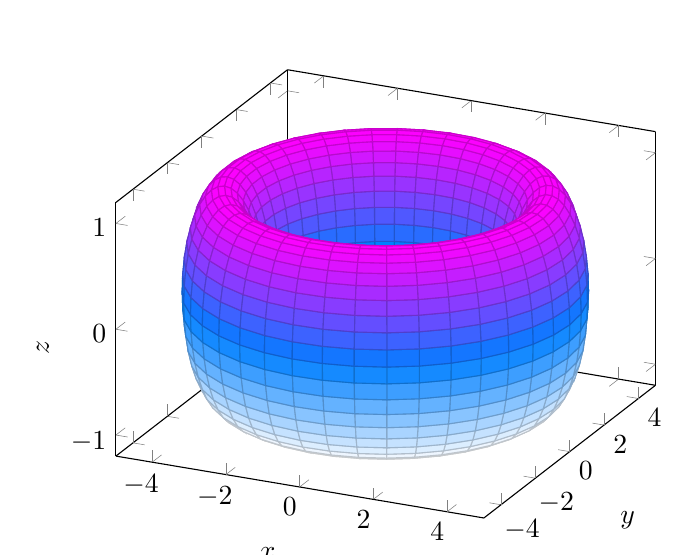
\begin{tikzpicture}
        \begin{axis}[xlabel = $x$,
            ylabel = $y$,
            zlabel = {$z$},]
        \addplot3[surf,
        colormap/cool,
        samples=40,
        domain=0:2*pi,y domain=0:2*pi,
        z buffer=sort]
        ({(4+cos(deg(x)))*cos(deg(y))}, 
            {(4+cos(deg(x)))*sin(deg(y))}, 
            {sin(deg(x))});
        \end{axis}
    \end{tikzpicture}
    \caption{Primer torusa iz zgleda \ref{zgl:9}}
\end{figure}


\subsection{Posplošen $n$-terni integral}

Do sedaj sta v integralu $\int_A f(x)\, dx$ nastopala omejena funkcija $f: A \to \R$ 
in omejena množica $A$. Če vsaj eden od njiju ni omejen, govorimo o posplošenem Riemannovem integralu 
(če ta obstaja).
Za množico $A \subseteq \R^n$ predpostavimo, da velja $m(\partial A) = 0$,
funkcijo $f$ pa razširimo na $\R^n$ z vrednostmi $0$ zunaj $A$, torej vpeljemo $\widetilde{f} = f \cdot \chi_A$.
Naj bo $f$ zvezna skoraj povsod na $A$.
Torej je tudi $f \cdot \chi_A$ zvezna skoraj povsod na $\R^n$.
Naj bo $P$ množica vseh točk $x \in \R^n$, za katere velja, da $f$ ni omejena v nobeni njihovi okolici.
Hitro sledi, da je $P$ zaprta podmnožica z mero $0$, saj je vsebovana v množici točk nezveznosti $f$.
Naj bo $\mathcal{K}_f$ množica vseh kompaktnih množic $Q \subseteq \R^n \setminus P$ s prostornino.

\begin{trditev}
    Če je $Q \in \mathcal{K}_f$, potem obstaja $\int_Q f(x)\, dx$.
\end{trditev}

\begin{dokaz}
    Na $Q$ je $f$ omejena, saj ima vsaka točka $x \in Q$ okolico, na kateri je $f$ omejena.
    Ker je $Q$ kompaktna, lahko izberemo končno podpokritje teh okolic in $f$ je na $Q$ omejena.
    Ker je $f$ zvezna skoraj povsod in je $V(\partial Q) = 0$, sledi integrabilnost.
\end{dokaz}

\begin{definicija}
    Naj bo $f$ nenegativna na $A$.
    Potem definiramo $$\int_A f(x)\, dx = \sup_{Q \in \mathcal{K}_f} \int_Q f(x)\, dx.$$
\end{definicija}

\begin{opomba}
    Ta integral je potencialno lahko tudi neskončen.
\end{opomba}

\begin{definicija}
    Naj bo $\Omega \subseteq \R^n$ odprta podmnožica.
Zaporedje kompaktnih podmnožic $K_1, K_2, \dots$ izčrpa odprto množico $\Omega$, če 
velja 
$$K_1 \subseteq \inte\, (K_2) \subseteq K_2 \subseteq \inte\, (K_3) \subseteq \dots$$
in $\bigcup K_j = \Omega$.
\end{definicija}

 Hitro vidimo, da za vsako odprto podmnožico $\Omega \subseteq \R^n$ 
obstaja zaporedje kompaktnih podmnožic, ki izčrpajo $\Omega$:
$$K_j = \overline{K(0, j)} \cap \left\lbrace x \in \Omega;\ d(x, \stcomp{\Omega}) \geq \frac{1}{j}\right\rbrace.$$
Izkaže pa se, da lahko te množice izbiramo tako, da imajo prostornino.
Denimo sedaj, da imamo izčrpanje $\R^n \setminus P$ s kompaktnimi podmnožicami s prostornino 
$(K_j)_j$. Naj bo $f(x) \geq 0$. Potem je zaporedje integralov $\int_{K_j} f(x)\, dx$ 
naraščajoče in obstaja (posplošena) limita $\lim_{j \to \infty} \int_{K_j} f(x)\, dx$.
Poleg tega za vsak kompakt $Q \in \mathcal{K}_f$ obstaja $j_0$, da velja $Q \subseteq K_{j_0}$,
saj notranjosti $\inte\; (K_j)_{j \in \N}$ tvorijo pokritje $Q$.
Zato velja $\int_Q f(x) \leq \int_{K_{j_0}} f(x)\, dx$, zato velja naslednja trditev.

\begin{trditev}
    Naj bo $f \geq 0$ na $A$ oziroma $\R^n$. Naj bo $f$ zvezna skoraj povsod.
    Naj zaporedje kompaktov s prostorninami $(K_j)_{j \in \N} \subseteq \mathcal{K}_f$ izčrpa $\R^n \setminus P$.
    Tedaj je $\int_Q f(x)\, dx = \lim_{j \to \infty} \int_{Q_{j}} f(x)\, dx$.
\end{trditev}

\begin{zgled}
    Izračunajmo integral $f(x, y) = e^{-(x^2 + y^2)}$ na $A = \R^2$.
    Izbiramo lahko bodisi $K_j = [-j, j] \times [-j, j]$ bodisi $\widetilde{K}_j = \overline{K(0, j)}$.
    Potem je 
    \begin{align*}
        \iint_{\R^2} e^{-(x^2 + y^2)}\, dx\, dy &= \lim_{j \to \infty} \iint_{K_j} e^{-(x^2 + y^2)}\, dx\, dy\\
        &= \lim_{j \to \infty} \iint_{\widetilde{K}_j} e^{-(x^2 + y^2)}\, dx\, dy.
    \end{align*}
    V prvem primeru je to 
    \begin{align*}
        \iint_{K_j} e^{-(x^2 + y^2)}\, dx\, dy &= \int_{-j} ^j e^{-x^2} \left(\int_{-j} ^j e^{-y^2}\, dy\right)\, dx\\
        &= \left(\int_{-j} ^j e^{-x^2}\, dx\right) \left(\int_{-j} ^j e^{-y^2}\, dy\right)
    \end{align*}
    in v limiti dobimo $\left(\int_{-\infty} ^\infty e^{-t^2}\, dt\right)^2 = \left(\Gamma \left(\frac{1}{2}\right)\right)^2$.
    Po drugi strani pa je 
    \begin{align*}
        \iint_{\widetilde{K}_j} e^{-(x^2 + y^2)}\, dx\, dy &=\int_0 ^{2\pi} \int_0 ^{j} e^{-r^2} r\, dr\, d\varphi\\
        &= 2 \pi \left(-\frac{1}{2} e^{-r^2}\right)\Big|_0 ^j\\
        &= \pi \left(1 - e^{-j^2}\right)
    \end{align*}
    in v limiti zopet dobimo $\pi$.
\end{zgled}

Naj bo sedaj $f$ poljubnega predznaka. Definirajmo funkciji $f^+ = \max\{f, 0\}\geq 0$
in $f^- = \max \{-f, 0\} \geq 0$.
Tedaj velja $f = f^+ + f^-$ in $|f| = f^+ + f^-$.
Funkcije $f^+$, $f^-$ in $|f|$ so lahko nezvezne le tam, kjer je $f$ nezvezna, torej so zvezne skoraj povsod.

\begin{definicija}
    Funkcija $f$ je absolutno integrabilna na $A$, če je $\int_A |f|\, dx < \infty$.
    To je ekvivalentno temu, da sta integrala $\int_A f^+ (x)\, dx < \infty$ in 
    $\int_A f^- (x)\, dx < \infty$ končna, saj $|f| = f^+ + f^-$.
    Potem definiramo $$\int_A f(x)\, dx = \int_A f^+ (x)\, dx - \int_A f^- (x)\, dx.$$
\end{definicija}

\begin{zgled}
    Izračunajmo $\iiint_{\overline{K(0, 1)}} \frac{1}{x^2 + y^2 + z^2}\, dx\, dy\, dz$.
    Tedaj je $P = \{(0, 0, 0)\}$ in vzamemo $K_j = \overline{K(0, j)} \setminus K\left(0, \frac{1}{j}\right)$
    za $j \in \N$. Potem je 
    \begin{align*}
        \iiint_{\overline{K(0, j)} \setminus K\left(0, \frac{1}{j}\right)} \frac{1}{x^2 + y^2 + z^2}\, dx\, dy\, dz 
        &= \int_0 ^{2\pi} \int_0 ^\pi \int_{\frac{1}{j}} ^1 \frac{r^2 \sin \theta}{r^2} \, dr\, d\theta\, d\varphi\\
        &= 2 \pi \left(1 - \frac{1}{j}\right) (-\cos \theta)\Big|_0 ^\pi\\
        &= 4 \pi \left(1 - \frac{1}{j}\right)
    \end{align*}
    in v limiti dobimo $4\pi$.
\end{zgled}

Množico vseh absolutno integrabilnih funkcij na $A$ označimo z $\mathcal{L}^1 (A)$.
Očitno je to vektorski prostor nad $\R$. Če si pogledamo funkcijo $f \in \mathcal{L}^1 \mapsto \int_A |f|\, dx$,
opazmo, da ima vse lastnost norme razen pozitivne definitnosti.
Zato vpeljemo ekvivalenčno relacijo na $\mathcal{L}^1 (A)$, da je $f \sim g \Leftrightarrow f = g$ skoraj povsod.
Sedaj tvorimo prostor ekvivalenčnih razredov $L^1 (A) = \quot{\mathcal{L}^1 (A)}{\sim}$.
Tako je integral dobro definiran funkcional na $L^1 (A)$ in 
$\| f\|_1 = \int_A |f|\, dx$ je norma na $L^1 (A)$.

\clearpage
\section{HARMONIČNA ANALIZA}

\subsection{Hilbertov prostor}

\begin{definicija}
    Vektorki prostor s skalarnim produktom, ki je v metriki, porojeni s skalarnim produktom 
    poln metrični prostor.
\end{definicija}

\begin{opomba}
    Normiranemu vektorskemu prostoru $(V, \|,\|)$, ki je z inducirano metriko poln, pravimo Banachov prostor.
\end{opomba}

\begin{zgled}
    Vzemimo vektorski prostor $\R^n$ z običajnim skalarnim produktom
    $\sprod{x}{y} = x_1 y_1 + \dots + x_n y_n$
    za $x = (x_1, \dots, x_n)$ in $y = (y_1, \dots, y_n)$.
    Tako dobimo metriko $d_2$ in vemo, da je $(\R^n, d_2)$ poln metrični prostor,
    torej je to Hilbertov prostor. Enako velja za prostor $\C^n$ s kanoničnim skalarnim produktom.
    Po drugi strani pa so normirani prostori $(\R^n, \|,\|_1)$, $(\R^n, \|,\|_\infty)$ 
    in $(C([a, b]), \|,\|_\infty)$ Banachovi.
\end{zgled}

\begin{zgled}\label{zgl:5}
    Naj bo $[a, b] \subseteq \R$ in vektorski prostor $V = C([a, b])$.
    Na njem imamo skalarni produkt $\sprod{f}{g} = \int_a ^b f(x) g(x)\, dx$ nad $\R$
    (oziroma $\sprod{f}{g} = \int_a ^b f(x) \overline{g(x)}\, dx$ nad $\C$).
    Vendar pa metrični prostor, ki ga ta skalarni produkt inducira, ni metričen.
    Protiprimer je na primer Cauchyjevo zaporedje 
    $$f(x) = \begin{cases}
        1; & \frac{1}{n} \leq x \leq 1\\
        nx; & -\frac{1}{n} \leq x \leq \frac{1}{n}\\
        -1; & -\frac{1}{n} \geq x \geq -1
    \end{cases},$$
    ki ne konvergira v prostoru $C([-1, 1])$.
\end{zgled}

% SLIKA %

Rešitev je napolnitev prostora $(C([a, b]), d_2)$ na prostor s kvadratom integrabilnih funkcij.
To je poln vektorski prostor $L^2 ([a, b])$ s skalarnim produktom 
$\sprod{f}{g} = \int_a ^b f(x) g(x)\, dx$, kjer je $-\infty \leq a < b \leq \infty$.
Prostoru $(C([a, b]), d_2)$ tako dodamo vse limite Cauchyjevih zaporedij.
Seveda je tudi $L^2 ([a, b])$ prostor ekvivalenčnih razredov relacije $$f \sim g \Leftrightarrow f = g\ \mathrm{\text{skoraj povsod}}.$$
S tem dve funkciji proglasimo za enaki, če sta enaki skoraj povsod. Tako dobimo prostor 
$$L^2 ([a, b]) = \left\lbrace f: [a, b] \to \R;\ \int_a ^b f^2 (x)\, dx < \infty\right\rbrace.$$
\vspace*{-5mm}
\begin{opomba}
    To je res vektorski prostor, saj za $f, g \in L^2 ([a, b])$ iz $|f \cdot g| \leq \frac{1}{2} (|f|^2 + |g|^2)$
sledi $f \cdot g \in L^1 ([a, b])$ in posledično 
$$\int_a ^b |f + g|^2 \, dx = \int_a ^b (|f|^2 + 2fg + |g|^2)\, dx < \infty.$$
Če velja $-\infty < a < b < \infty$, so vse zvezne in odsekoma zvezne funkcije na $[a, b]$ v tem prostoru.
\end{opomba}
Torej je $(L^2 ([a, b]), \langle , \rangle)$ Hilbertov prostor, ki ga dobimo z napolnitvijo prostora zveznih funkcij 
v metriki, ki jo porodi skalarni produkt. V prostoru $L^2 ([a, b])$ z $d_2$ metriko
$$d_2 (f, g) = \sqrt{\int_a ^b |f(x) - g(x)|^2\, dx}$$ je prostor $C([a, b])$ gost.
Torej lahko za vsako funkcijo $f \in L^2 ([a, b])$ in vsak $\varepsilon > 0$ obstaja zvezna funkcija 
$\widetilde{f} \in C([a, b])$, da je $d_2 (f, \widetilde{f}) < \varepsilon$.
Tako lahko dobimo zaporedje zveznih funkcij, ki v $d_2$ metriki konvergirajo k $f$.

Naj bo sedaj $X$ vektorski prostor s skalarnim produktom $\langle, \rangle$,
normo $\| x \| = \sqrt{\sprod{x}{x}}$ in metriko $d(x, y) = \| x - y\|$.
Skalarni produkt nam daje pojem pravokotnosti: vektorja $x, y \in X$ sta pravokotna natanko tedaj,
ko je $\sprod{x}{y} = 0$. Ta relacija je seveda simetrična.

\begin{trditev}
    Naj bodo $x_1, \dots, x_n \in (X, \langle,\rangle)$ paroma pravokotni, torej 
    $\sprod{x_i}{x_j} = 0$ za $i \neq j$. Tedaj velja 
    $$\|x_1 + \dots + x_n\|^2 = \|x_1\|^2 + \dots + \|x_n\|^2.$$
\end{trditev}

\begin{dokaz}
    \begin{align*}
        \|x_1 + \dots + x_n \|^2 &= \sprod{x_1 + \dots + x_n}{x_1 + \dots + x_n}\\
        &= \sum_i \sum_j \sprod{x_i}{x_j}\\
        &= \sum \sprod{x_i}{x_i}\\
        &= \|x_1\|^2 + \dots + \|x_n\|^2 \qedhere
    \end{align*}
\end{dokaz}

\begin{definicija}
    Za $A \subseteq X$ definiramo ortogonalni komplement 
$A^\perp = \{y \in X;\ \sprod{x}{y} = 0,\ \forall x \in A\}.$
\end{definicija}

\begin{trditev}
    $A^\perp$ je vektorski podprostor.
\end{trditev}

Vemo, da velja $A \subseteq (A^\perp)^\perp$, zanima pa nas,
ali v primeru, ko je $A$ podprostor, velja $A = (A^\perp)^\perp$.
V splošnem to ni res. 

\begin{trditev}
    $A^\perp$ je zaprt vektorski podprostor 
v $(X, \langle,\rangle)$.
\end{trditev} 

\begin{dokaz}
    Velja $| \sprod{x}{a} - \sprod{y}{a}| = |\sprod{x - y}{a}| \leq \|x - y\| \|a\|$.
    Funkcional $x \mapsto \sprod{x}{a}$ je torej zvezen. Če je $(x_j)_j \in A^\perp$ 
    in $\lim_{j \to \infty} x_j = x_0$, potem za vsak $a \in A$ velja $\sprod{x_j}{a} = 0$ in 
    $
        \lim_{j \to \infty} \sprod{x_j}{a} = \sprod{x_0}{a}
        = 0
    $, zato $x_0 \in A^\perp$.
\end{dokaz}

\begin{zgled}
    Naj bo $A = C([a, b]) \leq L^2 ([a, b])$. Vzemimo poljuben $f \in A = C([a, b])^\perp$.
    Po definiciji velja $\sprod{f}{g} = 0$ za $\forall g \in C([a, b])$.
    Sedaj vzemimo poljuben $F \in L^2 ([a, b])$. Potem obstaja zaporedje $(g_j)_j \in C([a, b])$,
    da je $\lim_{j \to \infty} g_j = F$ v $L^2$ smislu. Od tod pa sledi, da velja $\sprod{f}{F}$ za poljuben $F \in L^2([a, b])$,
    torej je $A^\perp = \{0\}$ in $(A^\perp)^\perp = L^2 ([a, b]) \neq A$.
\end{zgled}

\begin{opomba}
    Če je $(X, \langle,\rangle)$ Hilbertov prostor in $A \leq X$ zaprt podprostor,
    potem velja $(A^\perp)^\perp = A$.
\end{opomba}

\begin{definicija}
    Naj bo $(X, \langle, \rangle)$ vektorski prostor s skalarnim produktom in
    $Y \leq X$ njegov podprostor. Naj bo $x \in X$.
    Pravokotna projekcija $x$ na $Y$, če obstaja, je tak vektor $P_Y (x) \in Y$, da je 
    $x - P_Y x \in Y^\perp.$    
\end{definicija}

\begin{trditev}
    Naj bo $(X, \langle, \rangle)$ vektorski prostor s skalarnim produktom in
$Y \leq X$ njegov podprostor. Naj bo $x \in X$. Če obstaja pravokotna projekcija $x$ na $Y$, je enolično določen $P_Y (x)$ 
in velja, da je $P_Y (x)$ najboljša aproksimacija vektorja $x$ z vektorji iz $Y$:
$\inf_{w \in Y} \|x - w\| = \min_{w \in Y} \| x - P_Y(x)\|.$
Hkrati pa velja tudi $\|P_Y(x)\| \leq \|x\|.$
\end{trditev}

\begin{opomba}
    Naj bo $Y = C([a, b]) \leq L^2 ([a, b])$ in $f \in L^2 ([a, b])$.
    Potem je $P_y (f)$ najboljša aproksimacija $f$ s funkcijami iz $C([a, b])$.
    Če je $f \in L^2 ([a, b]) \setminus C([a, b])$, potem projekcija funkcije $f$ na $C([a, b])$ ne obstaja.
\end{opomba}

Denimo, da je za nek $Y \leq X$ pravokotna projekcija $P_Y (x)$ definirana za vsak $x \in X$.
Potem je $P_Y$ linearen in posledično tudi zvezen operator: za $x_1, x_2 \in X$ velja 
\begin{align*}
    \|P_Y (x_1) - P_Y (x_2)\| = \|P_Y (x_1 - x_2)\|
    = \|x_1 - x_2\|.
\end{align*}
Torej je operatorska norma $\|P_Y\| = 1$ za $Y \neq \{0\}$ in $P_Y ^2 = P_Y$.
Od tod hitro sledi, da če $P_Y (x)$ obstaja za vsak $x \in X$, je $Y$ zaprt podprostor.
Če je $Y \leq X$ in za vsak $x \in X$ obstaja $P_Y(x)$, potem velja $P_{Y^\perp} (x) = x - P_Y (x) = (I - P_Y)(x)$.

\begin{opomba}
    Če je $(X, \langle,\rangle)$ Hilbertov, $Y$ pa zaprt podprostor, potem za vsak $x \in X$
    obstaja pravokotna projekcija $P_Y (x) \in Y$.
\end{opomba}

\begin{trditev}
    Naj bo $Y \leq (X, \langle, \rangle)$ končno dimenzionalni prostor. Naj bo $e_1, \dots, e_n$ 
    ortonormirana baza $Y$. Naj bo $x \in X$. Tedaj je $P_Y = \sum_1 ^n \sprod{x}{e_j} e_j$.
\end{trditev}

\begin{definicija}
    Naj bo $\{e_j\}_{j \in J}$ družina neničelnih vektorjev. Potem je $\{e_j\}_{j\in J}$
    ortonormiran sistem (OS), če za vsaka $i \neq j$ velja $e_i \perp e_j$ oziroma ekvivalentno $\sprod{e_i}{e_j} = 0.$
    Naprej: $\{e_j\}_{j \in J}$ je ortonormiran sistem (ONS), če za vsaka $i, j$ velja 
    $$\sprod{e_i}{e_j} = \delta_{ij} = \begin{cases}
        1; & i = j\\
        0; & i \neq j
    \end{cases}.$$
\end{definicija}

\begin{trditev}[Besselova neenakost]
    Naj bo $(X, \langle, \rangle)$ vektorski prostor s skalarnim produktom.
    Naj bo $(e_j)_{j \in \N}$ ONS v $(X, \langle,\rangle)$. Naj bo $x \in X$.
    Potem je $\sum_1 ^\infty |\sprod{x}{e_j}|^2 \leq \|x\|^2$.
\end{trditev}

\begin{opomba}
    Zaporedje $(\sprod{x}{e_j})_j$ sestavljajo Fourierjevi koeficienti vektorja $x$ glede na $(e_j)_{j}$.
\end{opomba}

\begin{posledica}
    $\lim_{j \to \infty} \sprod{x}{e_j} = 0.$
\end{posledica}

\begin{dokaz}
    Naj bo $Y_n = \mathcal{L} (\{e_1, \dots, e_n\})$ in $e_1, \dots, e_n$ je ON baza $Y_n$.
    Potem za $\forall x \in X$ velja $P_{Y_n} (x) = \sum_1 ^n \sprod{x}{e_j} e_j$.
    Po Pitagorovem izreku je 
    \begin{align*}
        \sum_1 ^n \| \sprod{x}{e_j}^2 \| &= \sum_1 ^n \| \sprod{x}{e_j} \|^2 \|e_j\|^2\\
        &= \|P_{Y_n} (x) \|^2 \leq \|x\|^2
    \end{align*}
    in v limiti $n \to \infty$ dobimo $\sum_1 ^\infty |\sprod{x}{e_j}|^2 \leq \|x\|^2$.
\end{dokaz}

Sedaj se preselimo v Hilbertov prostore.

\begin{trditev}\label{trd:2}
    Naj bo $(X, \langle, \rangle)$ Hilbertov prostor.
    Naj bo $(c_j)_{j}$ zaporedje števil ($\R$, $\C$), da velja $\sum_1 ^\infty |c_j|^2 < \infty$.
    Naj bo $(e_j)_j$ ONS. Obstaja vektor $x \in X$, da je:
    \begin{enumerate}
        \item $x = \sum_1 ^\infty c_j e_j = \lim_{n \to \infty} \sum_1 ^n c_j e_j$ in 
        \item $\sprod{x}{e_j} = c_j$ za $\forall j$.
    \end{enumerate}
\end{trditev}

\begin{dokaz}
    Naj bo $x_n = \sum_1 ^n c_j e_j$. Dokazujemo, da je zaporedje delnih vsot Cauchyjevo.
    Vzemimo $n, p \in \N$. Potem je 
    \begin{align*}
        \|x_{n + p} - x_n\|^2 = \|\sum_{n + 1} ^{n + p} c_j e_j\|^2
        = \sum_{n + 1} ^{n + p} |c_j|^2 \|e_j\|^2
        = \sum_{n + 1} ^{n + p} |c_j|^2.
    \end{align*}
    Delne vsote $\sum_1 ^\infty |c_j|^2$ tvorijo Cauchyjevo zaporedje na $\R$, torej je zaporedje $x_n$ Cauchyjevo.
    Ker je $(X, \langle,\rangle)$ Hilbertov, obstaja $\lim_{n \to \infty} = \sum_1 ^\infty c_j e_j$.
    Še druga točka:
    \begin{align*}
        \sprod{x}{e_k} = \sprod{\sum_1 ^\infty c_j e_j}{e_k} &= \sprod{\lim_{n \to \infty} x_n}{e_k}\\
        &= \lim_{n \to \infty} \sprod{x_n}{e_k} = c_k \qedhere
    \end{align*}
\end{dokaz}

Naj bo $(X, \langle, \rangle)$ Hilbertov in $(e_j)_{j}$ njegov ONS.
Naj bo $x \in X$.
Vektorju $x$ priredimo njegove Fourierjeve koeficiente $(\sprod{x}{e_j})_{j = 1} ^\infty$.
Za njih velja $\sum_1 ^\infty |\sprod{x}{e_j}|^2 \leq \|x\|^2$ po Besselovi neenakosti, torej obstaja 
torej obstaja vektor $\widetilde{x} = \sum_1 ^\infty \sprod{x}{e_j}e_j \in X$. 
V splošnem $\widetilde{x}$ ni enak $x$.

\begin{definicija}
    ONS $(e_j)_{j}$ je kompleten ali poln ortonormiran sistem (KONS), če za vsak $x \in X$ velja 
    $x = \sum_1 ^\infty \sprod{x}{e_j} e_j$.
\end{definicija}

\begin{izrek}
    Naj bo $(e_j)_j$ ONS v Hilbertovem prostoru $(X, \langle,\rangle)$. Potem so naslednje trditve ekvivalentne.
    \begin{enumerate}
        \item $(e_j)_j$ je KONS.
        \item Za $\forall x, y \in X$ je $\sprod{x}{y} = \sum_1 ^\infty \sprod{x}{e_j} \overline{\sprod{y}{e_j}}$.
        \item Za vsak $x \in X$ je $\| x\|^2 = \sum_1 ^\infty |\sprod{x}{e_j}|^2$ (Parsevalova enakost).
        \item $(e_j)_j$ ni vsebovan v nobenem strogo večjem ONS.
        \item Edini vektor, ki je pravokoten na vse $(e_j)_j$, je vektor $0$.
        \item Končne linearne kombinacije vektorjev $(e_j)_j$ so goste v $(X, \langle,\rangle)$.
    \end{enumerate}
\end{izrek}

\begin{dokaz}
    Dokažimo $(6) \Rightarrow (5)$.
    Naj bo $x \in X$ pravokoten na vse $(e_j)_j$ in naj bo $\varepsilon > 0$.
    Naj bo $\sum_1 ^N \lambda_j e_j$ linearna kombinacija vektorjev $(e_j)_j$, da je 
    $\|x - \sum_1 ^N \lambda_j e_j\| < \varepsilon$. Tedaj velja 
    \begin{align*}
        \| x\|^2 = \sprod{x}{x} &= \sprod{x - \sum_1 ^N \lambda_j e_j}{x}\\
        &\leq \|x - \sum_1 ^N \lambda_j e_j\| \cdot \|x\|.
    \end{align*}
    Če $\|x\| \neq 0$, od tod dobimo $\|x\| \leq \|x - \sum_1 ^N \lambda_j e_j\|$
    in to za vsak $\varepsilon > 0$. Torej je $\|x\| = 0$ in zato $x = 0$.
\end{dokaz}

\subsection{Fourierove vrste}

Sedaj se omejimo na prostor $L^2 ([-\pi, \pi]) = L^2 (-\pi, \pi)$.
V tem kontekstu vsako funkcijo $f: [-\pi, \pi] - \R$ obravnavamo kot zožitev periodične funkcije s periodo $2 \pi$ na $\R$: $f(x + 2\pi) = f(x)$.
Pokazali bomo, da je množica $\left\lbrace\frac{1}{\sqrt{2\pi}},\ \frac{1}{\sqrt{\pi}} \cos(nx),\ \frac{1}{\sqrt{\pi}} \sin(nx)\right\rbrace_{n \in \N}$ KONS 
nad $\R$.
Očitno je, da ti vektorji tvorijo ONS: preverimo dve izmed možnih kombinacij, na primer
\begin{gather*}
    \int_{-\pi} ^{\pi} \frac{1}{\pi} \cos^2 (nx)\, dx = \frac{1}{\pi} \int_{-\pi} ^\pi \frac{1 + \cos(2nx)}{2}\, dx = 1
\end{gather*}
in $$\frac{1}{\pi} \int_{-\pi} ^\pi \cos(nx) \sin(mx)\, dx = \frac{1}{2\pi} \int_{-\pi} ^\pi (\sin ((n + m)x) + \sin ((m - n)x))\, dx = 0.$$
Če delamo na $\C$, pa bi lahko kot KONS izbrali $\left\lbrace \frac{1}{2\pi} e^{inx} \right\rbrace_{n \in \Z}$.
Sedaj definirajmo klasične Fourierjeve koeficiente. Ti so $a_n = \frac{1}{\pi} \int_{-\pi} ^\pi f(x)\cos (nx)\, dx$ za $n \in \N \cup \{0\}$
in $b_n = \frac{1}{\pi} \int_{-\pi} ^\pi f(x)\sin (nx)\, dx$ za $n \in \N$.
Formule za koeficiente so smiselne, ker velja $a_n = \frac{1}{\sqrt{\pi}} \sprod{f}{\frac{\cos (nx)}{\sqrt{\pi}}}$
in $b_n = \frac{1}{\sqrt{\pi}} \sprod{f}{\frac{\sin (nx)}{\sqrt{\pi}}}$ za $n \in \N$ in 
$a_0 = \frac{\sqrt{2}}{\sqrt{\pi}} \sprod{f}{\frac{1}{\sqrt{2\pi}}}$.

\begin{trditev}
    Za vsako funkcijo $f \in L^2 (-\pi, \pi)$ velja:
    \begin{itemize}
        \item $f(x) = \frac{a_0}{2} + \sum_1 ^\infty a_n \cos (nx) + b_n \sin (nx)$ v prostoru $L^2 (-\pi, \pi)$.
        \item $\frac{1}{\pi} \int_{-\pi} ^\pi |f(x)|^2\, dx = \frac{|a_0|^2}{2} + \sum_1 ^\infty (|a_n|^2 + |b_n|^2)$ (Parsevalova enakost).
    \end{itemize}
\end{trditev}

\begin{posledica}[Riemann-Lebesgueove lema]
    Iz tega, da je $\left\lbrace\frac{1}{\sqrt{2\pi}},\ \frac{1}{\sqrt{\pi}} \cos(nx),\ \frac{1}{\sqrt{\pi}} \sin(nx)\right\rbrace_{n \in \N}$ ONS sledi, da je
    $\lim_{n \to \infty} a_n = 0$ in $\lim_{n \to \infty} b_n = 0$.
\end{posledica}

\begin{izrek}
    Naj bo $f$ odsekoma zvezna in odsekoma odvedljiva periodična funkcija na $\R$ s periodo $2 \pi$.
    \begin{itemize}
        \item Na vsakem končnem intervalu ima $f$ končno mnogo točk nezveznosti in v vsaki točki $x_0 \in \R$
        obstajata $\lim_{x \uparrow x_0} f(x) = f(x_0 -)$ in $\lim_{x \downarrow x_0} f(x) = f(x_0 +)$.
        \item V vsaki točki $x_0 \in \R$ obstajata levi $\lim_{h \downarrow x_0} \frac{f(x_0-) - f(x-h)}{h}$ in desni odvod $\lim_{h \downarrow x_0} \frac{f(x+h) - f(x_0+)}{h}$.
    \end{itemize}
    Potem za vsak $x$ pripadajoča Fourierova vrsta konvergira po točkah in velja 
    $$\frac{f(x+) + f(x-)}{2} = \frac{a_0}{2} + \sum_1 ^\infty (a_n \cos (nx) + b_n \sin (nx)).$$
\end{izrek}

\begin{zgled}\label{zgl:6}
    Vzemimo funkcijo 
    $$f(x) = \begin{cases}
        1; & 0 < x \leq \pi\\
        0; & -\pi < x \leq 0
    \end{cases}.$$
    Potem je $a_0 = 1$, $a_n = 0$ in $b_n = \frac{1}{n \pi} (q - (-1)^n)$.
    Sedaj je $f(x) = \frac{1}{2} + \sum_{k = 0} ^\infty \frac{2}{(2k + 1)\pi} \sin ((2k + 1)x)$ in če vstavimo $x = \frac{\pi}{2}$, dobimo 
    $$1 - \frac{1}{3} + \frac{1}{5} - \dots = \frac{\pi}{4}.$$
    Velja pa tudi $\frac{1}{\pi}\int_{-\pi} ^\pi |f(x)|^2\, dx = 1$ in po Parsevalovi enakosti $1 = \frac{1}{2} + \sum_{k = 0} ^\infty \frac{4}{(2k + 1)^2\pi^2}$.
    Od tod pa sledi znana vsota: $$1 + \frac{1}{2^2} + \frac{1}{3^2} + \dots = \frac{\pi^2}{6}.$$
\end{zgled}

\begin{zgled}\label{zgl:7}
    Vzemimo funkcijo $f(x) = x$ na $[-\pi,\pi]$ (zunaj tega intervala pa periodična).
    Funkcija $f$ je liha, zato je $a_n = 0$ za $\forall n \in N$.
    Poračunamo še druge koeficiente in dobimo $b_n = \frac{2 (-1)^{n+1}}{n}$.
    Zato velja $f(x) = \sum_{1} ^\infty \frac{2}{n} (-1)^{n + 1} \sin (nx)$ za $x \neq -\pi, \pi$.
    Za $x = \pi$ pa dobimo $\sum_{1} ^\infty \frac{2}{n} (-1)^{n + 1} \sin (n\pi) = \frac{f(\pi+) + f(\pi-)}{2} = 0$.
\end{zgled}

Za dokaz izreka navedimo nekaj pomožnih trditev.

\begin{trditev}
    Naj bo $f: \R \to \R$ periodična s periodo $p$, torej velja $f(x + p) = f(x)$ za vse $x \in \R$.
    Naj bo $f$ integrabilna na vsakem končnem intervalu. Potem za $\forall a \in \R$ velja
    $$\int_a ^{a + p} f(x)\, dx = \int_0 ^p f(x)\, dx.$$ 
\end{trditev}

Definirajmo Dirichletovo jedro $D_N (x) = \frac{1}{2} + \sum_1 ^N \cos (nx)$.
Potem imamo 
\begin{align*}
    D_N (x) &= \frac{1}{2} + \sum_1 ^N \frac{e^{inx} + e^{-inx}}{2}  = \frac{1}{2} e^{-iNx} (1 + e^{ix} + \dots + e^{2iNx})\\
    &= \frac{1}{2} e^{-iNx} \frac{e^{(2N + 1)ix} - 1}{e^{ix} - 1}
    = \frac{1}{2} \frac{e^{(N + \frac{1}{2})ix} - e^{-(N + \frac{1}{2})ix}}{e^{\frac{ix}{2}} -e^{-\frac{ix}{2}}}\\
    &= \frac{\sin \left(\left(N + \frac{1}{2}\right)x\right)}{2\sin \left(\frac{x}{2}\right)}.
\end{align*}
Nadalje imamo $\frac{1}{\pi} \int_{-\pi} ^\pi D_n (x)\, dx = 1$ in $D_n$ je soda funkcija s periodo $2 \pi.$
Upoštevamo še dejstvo $$D_N = \frac{\sin \left(\left(N + \frac{1}{2}\right)x\right)}{2\sin \left(\frac{x}{2}\right)} = \frac{1}{2} \left(\frac{\cos \left(\frac{x}{2}\right)}{\sin \left(\frac{x}{2}\right)} \sin(Nx) + \cos(Nx)\right)$$
in lahko dokažemo izrek. 

\begin{dokaz}
    Definiramo $S_N(x) = \frac{a_0}{2} + \sum_1 ^\infty a_n \cos (nx) + b_n \sin (nx)$ in dobimo 
    \begin{align*}
        S_N &= \frac{1}{\pi} \int_{-\pi} ^\pi f(t) \left(\frac{1}{2} + \sum_1 ^N \cos (n(t - x))\right) \, dt\\
        &= \frac{1}{\pi} \int_{-\pi} ^\pi f(t) D_N (t - x)\, dt\\
        &\stackrel{t - x = v}{=} \frac{1}{\pi} \left(\int_0 ^\pi f(x + v) D_N (v)\, dv + \int_{0} ^\pi f(x - v) D_N (v)\, dv\right).
    \end{align*}
    Integralom oblike $(f * g) (x) = \int_{-\pi} ^\pi f(t) g(x-t)\, dt$ sicer pravimo konvolucije. Poglejmo razliko
    \begin{align*}
        S_N (x) - \frac{f(x+) + f(x-)}{2} &= S_N (x) - \frac{1}{\pi} \int_0 ^\pi (f(x+) + f(x-)) D_N (v)\, dv\\
        &= \frac{1}{\pi} \int_0 ^\pi (f(x + v) - f(x+)) D_N (v)\, dv\\ &+ \frac{1}{\pi} \int_0 ^\pi (f(x-v) - f(x-)) D_N (v)\, dv
    \end{align*}
    Oglejmo si prvi člen:
    \begin{align*}
        \frac{1}{\pi} \int_0 ^\pi (f(x + v) - f(x+)) D_N (v)\, dv &= \frac{1}{2\pi} \int_0 ^\pi (f(x + v)- f(x+)) \left(\frac{\cos \left(\frac{x}{2}\right)}{\sin \left(\frac{x}{2}\right)} \sin(Nx) + \cos(Nx)\right)\, dv\\
        &= \frac{1}{2\pi} \int_0 ^\pi \frac{(f(x + v)- f(x+))}{v} \frac{v}{\sin \left(\frac{x}{2}\right)}\cos \left(\frac{x}{2}\right) \sin(Nx)\, dv\\ 
        &+ \frac{1}{2\pi} \int_0 ^\pi \frac{(f(x + v)- f(x+))}{v} v \cos (Nv)\, dv
    \end{align*}
    Definirajmo funkcijo $$\widetilde{f} (v) = \begin{cases}
        \frac{1}{2} \frac{(f(x + v)- f(x+))}{v} \frac{v}{\sin \left(\frac{x}{2}\right)}\cos \left(\frac{x}{2}\right); & v > 0\\
        0; & v < 0
    \end{cases}.$$
    Po predpostavki obstaja $\lim_{v \downarrow 0} \frac{(f(x + v)- f(x+))}{v}$, zato je $\widetilde{f}$
    odsekoma zvezna in zato $\widetilde{f} \in L^2 (-\pi, \pi)$. Zato gre po Riemann-Lebesgueovi lemi ta sumand proti $0$, ko gre $N \to \infty$.
    Podobno lahko zaključimo za drugi sumand tega člena in pa tudi drugi člen.
\end{dokaz}

\begin{opomba}
    Če je $f$ liha funkcija, so $a_n = 0,\ \forall n \in \N$, če pa je $f$ soda funkcija,
    pa so $b_n = 0,\ \forall n \in \N$. To lahko izkoristimo za razvoj le po sinusih ali le po kosinusih.
    Primer take uporabe je recimo za funkcije $f: [0, \pi] \to \R$, ki jo razširimo bodisi do lihe bodisi do sode funkcije na $[-\pi, \pi]$.
\end{opomba}

\begin{opomba}
    Funkcije s periodo $p = 2l$ lahko na $[-l, l]$ razvijemo kot 
    $$f(x) = \frac{a_0}{2} + \sum_1 ^\infty a_n \cos \left(n \pi \frac{x}{l}\right) + b_n \sin \left(n \pi \frac{x}{l}\right),$$
    kjer je $a_n = \frac{1}{l} \int_{-l} ^l f(x) \cos \left(n \pi \frac{x}{l}\right) \, dx$ in 
    $b_n = \frac{1}{l} \int_{-l} ^l f(x) \sin \left(n \pi \frac{x}{l}\right) \, dx$.
\end{opomba}

\begin{figure}[htb!]
    \centering
    \begin{minipage}[b][7cm][s]{.45\textwidth}
    \centering
    \vfill
    \begin{tikzpicture}[scale=0.85]
        \begin{axis}[
            xmin=-1, xmax=1,
            ymin=-2, ymax=2,
            xtick={-1,0,1},
            ytick={-1,0,1},
            %ymajorgrids=true,
            %grid style=dashed,
        ]
        %\addplot[domain=0.0001:5] {x^(1/x)};
        
            \addplot[domain=-0.2:0.2] {(5*x)};
            \addplot[domain=-1:-0.2] {-1};
            \addplot[domain=0.2:1] {1};

            \addplot[domain=-2:2, color=gray, dashed] {0};
            \addplot[dashed, color=gray] coordinates {(0,-2)(0,2)};
        \end{axis}
    \end{tikzpicture}
    \caption{Zgled \ref{zgl:5}}
    \end{minipage}\qquad
    \begin{minipage}[b][7cm][s]{.45\textwidth}
    \centering
    \vfill
    \begin{tikzpicture}[scale=0.85]
        \begin{axis}[ 
            ymin=-2, ymax=2,
            ytick={-1,0,1},
            xmin=-2*pi, xmax=2*pi,
            xtick={-6.28318,-3.14159,0,3.14159,6.28318},
            xticklabels={$-2\pi$, $-\pi$, $0$, $\pi$,$2\pi$},
        ]
        \addplot[domain=-2*pi:-pi] {1};
        \addplot[domain=-pi:0] {0};
        \addplot[domain=0:pi] {1};
        \addplot[domain=pi:2*pi] {0};
        \addplot[domain=-2*pi:2*pi, color=gray, dashed] {0};
        \addplot[dashed, color=gray] coordinates {(0,-2)(0,2)};
        \end{axis}
        \end{tikzpicture}
    \caption{Zgled \ref{zgl:6}}
    \end{minipage}
    
    \begin{minipage}[b][7cm][s]{.45\textwidth}
    \centering
    \vfill
    \begin{tikzpicture}[scale=0.85]
        \begin{axis}[ 
            ymin=-2*pi, ymax=2*pi,
            ytick={-6.28318,-3.14159,0,3.14159,6.28318},
            yticklabels={$-2\pi$, $-\pi$, $0$, $\pi$,$2\pi$},
            xmin=-2*pi, xmax=2*pi,
            xtick={-6.28318,-3.14159,0,3.14159,6.28318},
            xticklabels={$-2\pi$, $-\pi$, $0$, $\pi$,$2\pi$},
        ]
        \addplot[domain=-2*pi:-pi] {2*pi + x};
        \addplot[domain=-pi:pi] {x};
        \addplot[domain=pi:2*pi] {-2*pi + x};
        \addplot[domain=-2*pi:2*pi, color=gray, dashed] {0};
        \addplot[dashed, color=gray] coordinates {(0,-2*pi)(0,2*pi)};
        \end{axis}
        \end{tikzpicture}
    \caption{Zgled \ref{zgl:7}}
    \end{minipage}\qquad
    \begin{minipage}[b][7cm][s]{.45\textwidth}
    \centering
    \vfill
    \begin{tikzpicture}[scale=0.85]
        \begin{axis}[ 
            ymin=-15, ymax=15,
            ytick={-10,-5,0,5,10},
            xmin=-2*pi, xmax=2*pi,
            xtick={-6.28318,-3.14159,0,3.14159,6.28318},
            xticklabels={$-2\pi$, $-\pi$, $0$, $\pi$,$2\pi$},
        ]
        \addplot[domain=-2*pi:-pi] {pi*pi - (x + 2*pi)^2};
        \addplot[domain=-pi:pi] {pi^2 - x^2};
        \addplot[domain=pi:2*pi] {pi*pi - (x - 2*pi)^2};
        \addplot[domain=-2*pi:2*pi, color=gray, dashed] {0};
        \addplot[dashed, color=gray] coordinates {(0,-15)(0,15)};
        \end{axis}
    \end{tikzpicture}
    {\caption{Zgled \ref{zgl:8}}}
    \end{minipage}
\end{figure}
    
\begin{zgled}\label{zgl:8}
    Vzemimo $f(x) = \pi^2 - x^2$.
    Če razvijemo po Fourieru, dobimo $b_n = 0,\ \forall n \in \N$,
    $a_0 = \frac{4 \pi^2}{3}$ in $a_n = \frac{4(-1)^{n + 1}}{n^2}$.
    Tako dobimo $\pi^2 - x^2 = \frac{2\pi^2}{3} + \sum_1 ^\infty \frac{4 (-1)^{n + 1}}{n^2} \cos(nx)$
    za vsak $x \in [-\pi, \pi]$. Če vstavimo $x = \pi$, ponovno dobimo 
    $$\frac{\pi^2}{6} = 1 + \frac{1}{2^2} + \frac{1}{3^2} + \dots$$
    Če pa vstavimo $x = 0$, dobimo 
    $$\frac{\pi^2}{12} = 1 - \frac{1}{2^2} + \frac{1}{3^2} - \dots$$
    Oglejmo si še Parsevalovo enakost: $\frac{1}{\pi} \int_{-\pi} ^\pi (\pi^2 - x^2)^2 \, dx = \frac{8 \pi^2}{9} + 16 \sum_1 ^\infty \frac{1}{n^4}$ in od tod 
    $$1 + \frac{1}{2^4} + \frac{1}{3^4} + \dots = \frac{\pi^4}{90}.$$
\end{zgled}

Definirajmo $F_N (x) = \frac{1}{N} \sum_0 ^{N - 1} D_N (x)$ kot Fejerjevo jedro.

\begin{trditev}
    Za Fejerjevo jedro veljajo naslednje lastnosti.
    \begin{itemize}
        \item $F_N (x) = \frac{1}{N} \left(\frac{\sin \left(\frac{Nx}{2}\right)}{\sin \left(\frac{x}{2}\right)}\right)^2$.
        \item $\frac{1}{\pi} \int_{-\pi} ^\pi F_N (x)\, dx = 1$.
        \item $F_N (x)$ za $\forall x \in [-\pi, \pi]$, soda.
        \item Za vsak $a \in (0, \pi)$ velja $\lim_{N \to \infty} F_N (x) = 0$ enakomerno na $[a, \pi]$.
    \end{itemize}
\end{trditev}

\begin{izrek}
    Naj bo $f$ zvezna $2\pi$-periodična funkcija.
    Potem Cesarjeve delne vsote 
    $\sigma_N (x) = \frac{1}{N} (S_0 (x) + \dots + S_{N - 1} (x))$ 
    konvergirajo k $f$ enakomerno na $[-\pi, \pi]$.
\end{izrek}

\begin{dokaz}
    Vemo, da je 
    \begin{align*}
        S_n (x) &= \frac{1}{\pi} \int_{-\pi} ^\pi f(x + y) \frac{\sin\left(\left(n + \frac{1}{2}\right)y\right)}{\sin \left(\frac{y}{2}\right)}\, dy\\
        &= \frac{1}{\pi} \int_{-\pi} ^\pi f(x + y) D_n (y)\, dy\\
        &= \frac{1}{\pi} \int_{-\pi} ^\pi f(t) D(x - t)\, dt.
    \end{align*}
    Torej je 
    \begin{align*}
        \sigma_N (x) &= \frac{1}{\pi} \int_{-\pi} ^\pi f(x + y) F_N (y)\, dy\\
        &= \frac{1}{\pi} \int_{-\pi} ^\pi f(t) F_N (x - t)\, dt.
    \end{align*}
    Naj bo $\varepsilon > 0$. Ker je $f$ zvezna periodična, je enakomerno zvezna na $\R$.
    Torej obstaja $\delta > 0$, da iz $|y| < \delta$ sledi 
    $|f(x + y) - f(x)| <\frac{\varepsilon}{2}$ za vsak $x \in \R$.
    Če upoštevamo $\frac{1}{\pi} \int_{-\pi} ^\pi F_N(y)\, dy = 1$ in $F_N \geq 0$,
    dobimo 
    \begin{align*}
        |\sigma_N (x) - f(x)| &= \frac{1}{\pi} \left| \int_{-\pi} ^\pi (f(x + y) - f(x)) F_N (y)\, dy \right|\\
        &\leq \frac{1}{\pi} \int_{-\pi} ^\pi \left| (f(x + y) - f(x)) \right| F_N (y)\, dy\\
        &\frac{1}{\pi} \int_{-\delta} ^\delta |f(x+y) - f(x)| F_N (y)\, dy \\
        &+\frac{1}{\pi} \int_{\delta \leq |y| \leq \pi} |f(x+y) - f(x)| F_N (y)\, dy.
    \end{align*}
    Ker je $f$ periodična in zvezna, je omejena na $\R$ in velja 
    $|f(t)| < M$ za vsak $t \in \R$. Vemo, da za $\delta \leq |y| \leq \pi$
    zaporedje $\{F_N\}$ konvergira enakomerno proti $0$. Torej lahko res oba člena ocenimo navzdol z
    $\frac{\varepsilon}{2}$ za dovolj velik $N$.
\end{dokaz}

\begin{opomba}
    Bolj gladka je periodična funkcija, hitreje konvergirajo Fourierove vsote proti $f$.
    Hitro vidimo, da so koeficienti $k$-krat zvezno odvedljive periodične funkcije velikostnega reda $O\left(\frac{1}{n} \right)$. 
\end{opomba}

\begin{opomba}[Carlesonov izrek]
    Če je $f$ zvezna periodična funkcija, njena Fourierova vrsta konvergira k $f(x)$
    (po točkah) skoraj povsod.
\end{opomba}

\begin{trditev}
    Ortonormiran sistem $\left\lbrace \frac{1}{\sqrt{2\pi}}, \frac{1}{\sqrt{\pi}} \cos(nx), \frac{1}{\sqrt{\pi}} \sin (nx) \right\rbrace_{n \in \N}$
    je kompleten v $L^2 (-\pi, \pi)$.
\end{trditev}

\begin{dokaz}
    Glede na prejšnji izrek lahko vsako zvezno periodično funkcijo poljubno dobro enakomerno aproksimiramo 
    s trigonometričnimi polinomi, tj. končnimi linearnimi kombinacijami funkcij 
    $\{1, \sin (nx), \cos (nx)\}$ za $n \in \N$.
    Vemo, da je prostor $L^2 (-\pi, \pi)$ napolnitev prostora $C([-\pi, \pi])$
    v metriki $d_2$ in se zato vsaka funkcija $f \in L^2$ da v tej metriki poljubno dobro aproksimirati z zveznimi funkcijami
    na $[-\pi, \pi].$ Naj bo torej $f \in C([-\pi, \pi])$ in za $n \in \N$ definiramo funkcijo 
    $$f_n (x) = \begin{cases}
        f(x); & -\pi + \frac{1}{n} \leq x \leq \pi - \frac{1}{n}\\
        -nf\left(\pi - \frac{1}{n}\right) (x - \pi); & \pi - \frac{1}{n} < x \leq \pi\\
        nf\left(-\pi + \frac{1}{n}\right) (x + \pi); & - \pi \leq x < - \pi + \frac{1}{n}
    \end{cases}.$$
    Potem je $f_n \in C([-\pi, \pi])$ in jo lahko razširimo na $\R$ kot zvezno periodično funkcijo.
    To funkcijsko zaporedje pa v $d_2$ metriki konvergura k $f$.
\end{dokaz}

\begin{figure}[hbt!]
    \centering
    \begin{tikzpicture}[scale=1.0]
        \begin{axis}[ 
            ymin=-1, ymax=4,
            ytick={0,1,2,3},
            xmin=-pi, xmax=pi,
            xtick={-3.14159,0,3.14159},
            xticklabels={$-\pi$, $0$, $\pi$},
        ]
        \addplot[domain=-pi:-pi + 0.2] {5*(sin(deg(1.3 - 1.5*pi)) + 2)*(x + pi)};
        \addplot[domain=-pi+0.2:pi-0.2] {(sin(deg(1.5*x + 1)) + 2)};
        \addplot[domain=pi-0.2:pi] {-5*(sin(deg(0.7 + 1.5*pi)) + 2)*(x - pi)};
        \addplot[domain=-2*pi:2*pi, color=gray, dashed] {0};
        \addplot[dashed, color=gray] coordinates {(0,-2*pi)(0,2*pi)};
        \end{axis}
        \end{tikzpicture}
    \caption{Primer razširitve na zvezno periodično funkcijo}
\end{figure}

\begin{posledica}[Weierstrassov izrek]
    Naj bo $f \in C([a, b])$. Potem lahko $f$ poljubno dobro enakomerno aproksimiramo s polinomi.
\end{posledica}

\begin{dokaz}
    Po raztegih in translacijah je dovolj, če dokažemo za primer $f \in C(\left[-\frac{\pi}{2}, \frac{\pi}{2}\right])$.
    Sedaj $f$ zvezno razširimo na $[-\pi, \pi]$ kot v prejšnjem dokazu:
    $$\widetilde{f} (x) = \begin{cases}
        f(x); & -\frac{\pi}{2} \leq x \leq \frac{\pi}{2}\\
    -\frac{2}{\pi}f\left(\frac{\pi}{2}\right) (x - \pi); & \frac{\pi}{2} < x \leq \pi\\
    \frac{2}{\pi}f\left(-\frac{\pi}{2}\right) (x + \pi); & -\pi \leq x < -\frac{\pi}{2}\\
    \end{cases}.$$
    Sedaj lahko $\widetilde{f}$ na $[-\pi, \pi]$ poljubno dobro enakomerno aproksimiramo s trigonometričnimi polinomi, slednje 
    pa lahko na $[-\pi, \pi]$ poljubno dobro enakomerno aproksimiramo s Taylorjevimi polinomi. 
\end{dokaz}

\subsection{Fourierova transformacija}

Pri Fourierovih vrstah smo vzeli periodično funkcijo $f \in L^2 (-\pi, \pi)$
in ji priredili koeficiente.
Naj bo tokrat KONS v $L^2 (-\pi, \pi)$ množica $\left\lbrace\frac{1}{\sqrt{2\pi}} e^{inx}\right\rbrace_{n \in \N}$.
Potem so Fourierovi koeficienti 
$$C_n = \hat{f} (n) = \sprod{f}{\frac{1}{\sqrt{2\pi}} e^{inx}} = \frac{1}{2\pi} \int_{-\pi} ^\pi f(x) e^{-inx}\, dx.$$
Dobimo zaporedje kompleksnih števil $\left(\hat{f} (n)\right)_{n \in \Z}$, 
kjer velja Parsevalova enakost:
$\sum_{-\infty} ^\infty |\hat{f} (n)|^2 = \int_{-\pi} ^\pi |f(x)|^2\, dx$.
Prostor $l^2$ je vektorski prostor kompleksnih zaporedij $(c_n)_{n \in \Z}$,
za katere velja $\|(c_n)\|_2 ^2 = \sum_n |c_n|^2 < \infty$.
Tudi ta prostor ima skalarni produkt $\sprod{(c_n)}{(d_n)} = \sum_n c_n \overline{d_n}$ 
in ker velja
\begin{align*}
    \left| \sum_{-N} ^N c_n \overline{d_n} \right|^2 \leq \left(\sum_{-N} ^N |c_n|^2\right) \left(\sum_{-N} ^N |d_n|^2\right) \leq \| (c_n)\|_2 ^2 \| (d_n) \|_2 ^2 < \infty,
\end{align*}
je ta skalarni produkt dobro definiran. Očitno je to tudi vektorski prostor nad $\C$ 
z metriko $d((c_n), (d_n))^2 = \sum_n |c_n - d_n|^2$.
Izkaže se, da je to tudi Hilbertov prostor, torej je Fourierova vrsta pravzaprav linearna preslikava 
med dvema Hilbertovima prostoroma $L^2 (-\pi, \pi) \to l^2$ s predpisom $f \mapsto (\hat{f}(n))_n$.
Po Parsevalovi enakosti je to izometrija, zato je injektivna. Surjektivnost pa sledi iz trditve \ref{trd:2}.

\begin{opomba}
    Ker opazujemo periodične funkcije, bi pravzaprav lahko opazovali funkcije na krožnici $S^1$.
\end{opomba}

Fourierova transformacija je definirana na kompleksnih funkcijah na $\R$.
Do sedaj smo spoznali prostora absolutno integrabilnih in s kvadratom integrabilnih funkcij na $[-\pi, \pi]$ 
in videli, da velja $L^2 (-\pi, \pi) \subseteq L^1 (-\pi, \pi)$,
ker je $$\int_{-\pi} ^\pi |f|\, dx = \int_{-\pi} ^\pi 1 \cdot |f|\, dx \leq \sqrt{\int_{-\pi} ^\pi 1^2\, dx} \sqrt{\int_{-\pi} ^\pi |f|^2\, dx}$$
oziroma $\|f\|_1 \leq \sqrt{2\pi} \|f\|_2$.

\begin{zgled}
    Funkcija $$f(x) = \begin{cases}
        \frac{1}{\sqrt{|x|}}; & x \neq 0\\
        0; & x = 0
    \end{cases}$$
    je primer funkcije, ki je v $L^1 (-\pi, \pi)$,
    ne pa v $L^2 (-\pi, >\pi)$.
    Pri prostorih $L^1 (\R)$ in $L^2 (\R)$ pa nimamo inkluzije  nobeno smer.
    Protiprimera sta recimo funkciji $g(x) = \frac{1}{1 + |x|}$ in
    $$f(x) = \begin{cases}
        \frac{1}{\sqrt{x}}; & 0 \leq x \leq 1\\
        0; & \mathrm{sicer}
    \end{cases}.$$ 
\end{zgled}

Oba prostora $L^1 (\R)$ in $L^2 (\R)$ sta napolnitev prostora zveznih funkcij v ustrezni metriki.
Množica $L_1 (\R) \cap L_2 (\R)$ je gost podprostor tako v $L^1 (\R)$ (v metriki $d_1$) kot tudi v $L^2 (\R)$ (v metriki $d_2$).
Tokrat začnemo s prostorom $L^1 (\R)$.

\begin{zgled}
    Navedimo nekaj primerov funkcij, ki so v preseku teh dveh prostorov.
    Na primer integrabilne funkcije, ki so zunaj končnega intervala ničelne (oziroma funkcije s končnim nosilcem),
    ali pa funkcije oblike $p(x) e^{-ax^2}$ ali $p(x) e^{-a|x|}$, kjer je $p$ polinom in $a > 0$.
    Opazimo, da so tudi vsi odvodi teh funkcij v preseku $L^1 (\R)$ in $L^2 (\R)$.
\end{zgled}

\begin{opomba}
    Prostor $L^1$ je Banachov.
\end{opomba}

Fourierova transformacija je preslikava $\F: L^1 (\R) \to L^\infty (\R)$,
definirana s predpisom $\F(f) (\xi) = \hat{f} (\xi) = \int_{-\infty} ^\infty e^{-2\pi i t \xi} f(t)\, dt$
za $\xi \in \R$. Opazimo, da je
$$
    |\hat{f}(\xi)| \leq \int_{-\infty} ^\infty |e^{-2\pi i t \xi} f(t)|\, dt \leq \int_{-\infty} ^\infty |f(t)|\, dt = \|f\|_1.
$$
Prostor $L^\infty (\R)$ je prostor bistveno omejenih funkcij na $\R$.
Za normo bi lahko definirali $\|g\|_\infty = \sup_\R |g|$ oziroma bistveni supremum.
Torej je $\| \hat{f} \|_\infty \leq \|f\|_1$.

\begin{zgled}
    Naj bo $$f(t) = \begin{cases}
        a; & -\frac{L}{2} \leq t \leq \frac{L}{2}\\
        0; & \mathrm{sicer}
    \end{cases}.$$
    Potem je njena Fourierova transformacija 
    \begin{align*}
        \hat{f} (\xi) = \int_{-\infty} ^\infty e^{-2 \pi i \xi t} f(t)\, dt &= a \int_{-\frac{L}{2}} ^\frac{L}{2} e^{-2\pi i \xi t}\, dt\\
        &= \frac{a}{\pi \xi} \left(\frac{e^{\pi i \xi L} - e^{-\pi i \xi L}}{2i}\right)\\
        &= \frac{a}{\pi \xi} \sin (\pi i \xi L).
    \end{align*}
    Opazimo, da je $\lim_{|\xi| \to \infty} \hat{f} (\xi) = 0$.
\end{zgled}

\begin{zgled}
    Naj bo $f(t) = e^{-a|t|}$ za $a > 0$. Njena Fourierova transformacija je
    \begin{align*}
        \hat{f} (\xi) &= \int_{-\infty} ^\infty e^{-2 \pi i \xi t} e^{-a|t|}\, dt\\
        &= \int_{-\infty} ^0 e^{(-2 \pi i \xi + a)t}\,dt + \int_0 ^\infty e^{(-2 \pi i \xi - a)t}\, dt\\
        &= \frac{2a}{a^2 + 4\pi^2 \xi^2}
    \end{align*}
    in tudi tokrat velja $\lim_{|\xi| \to \infty} \hat{f} (\xi) = 0$.
\end{zgled}

\begin{zgled}
    Račun iz prejšnjih dveh zgledov ponovimo še za funkcijo $f(t) = e^{-at^2}$, $a > 0$ (tokrat uporabimo rezultat iz poglavja o gama funkciji)
    in dobimo $\hat{f}(\xi) = \sqrt{\frac{\pi}{a}} e^{-\frac{\pi^2 \xi^2}{a}}$
    in $\lim_{|\xi| \to \infty} \hat{f} (\xi) = 0$.
    V $\hat{f} (\xi)= \sqrt{\frac{\pi}{a}} e^{-\frac{\pi^2 \xi^2}{a}}$ vstavimo $a = \pi$ in dobimo 
    $\F (e^{-\pi t^2}) (\xi) = e^{-\pi \xi^2}$.
    Torej je funkcija $t \mapsto e^{-\pi t^2}$ lastna funkcija Fouriereve transformacije za lastno vrednost $1$ (pozor: Fourierova transformacija, kot smo jo vpeljali, še ni endomorfizem -- glej nadaljevanje).
\end{zgled}

\begin{zgled}
    Oglejmo si $f(t) = \frac{a}{\pi} \frac{\sin (\pi L t)}{t}$. Ta funkcija sicer ni v $L^1 (\R)$,
    je pa v $L^2 (\R)$. Spomnimo se, da velja $\int_0 ^\infty \frac{\sin (ax)}{x}\, dx = \frac{\pi}{2} \mathrm{sgn}(a)$.
    Če poskusimo na $f$ uporabiti Fourierovo transformacijo, dobimo 
    $$\hat{f} (\xi) = \begin{cases}
        a ; & -\frac{L}{2} < \xi < \frac{L}{2}\\
        \frac{a}{2} ; & \xi = \frac{L}{2}\ \mathrm{ali}\ \xi = - \frac{L}{2}\\
        0 ; & \mathrm{sicer}
    \end{cases}.$$
\end{zgled}

\begin{opomba}
    Vse funkcije $f$ v zgledih so bile sode, zato je $\hat{f}$ bila realna funkcija:
    $$\hat{f} (\xi) = \int_{-\infty} ^\infty (\cos (2 \pi i \xi t) - i \sin (2 \pi i \xi t)) f(t)\, dt.$$ 
    Opazimo, da smo na funkciji $t \mapsto \chi_{\left[-\frac{L}{2}, \frac{L}{2}\right]} (t)$
    dvakrat uporabili Fourierovo transformacijo in dobili povprečja levih in desnih limit.
\end{opomba}

\begin{trditev}
    Osnovne lastnosti Fourierove transformacije:
    \begin{itemize}
        \item $\F: L^1 (\R) \to L^\infty (\R)$ je linearna preslikava in velja $\| \F (f)\|_{\infty} \leq \|f\|_1$.
        \item Za vsak $f \in L^1 (\R)$ je $\F (f)$ enakomerno zvezna na $\R$.
        \item Če je $f \in L^1 (\R)$ odvedljiva in je $f' \in L^1 (\R)$, je 
        $\F (f') (\xi) = (2 \pi i \xi) \F (f) (\xi)$. Podobno velja za višje odvode: če je $f \in L^1 (\R)$ 
        $n$-krat odvedljiva in velja $f', \dots, f^{(n)} \in L^1 (\R)$, potem je
        $\F (f^{(n)}) (\xi) = (2 \pi i \xi)^n \F (f) (\xi)$.
    \end{itemize}
\end{trditev}

\begin{opomba}
    Če je $f' \in L^1 (\R)$, potem je $\widehat{f'}$ omejena in zato dobimo 
    $\lim_{|\xi| \to \infty} \hat{f}(\xi) = \lim_{|\xi| \to \infty} \frac{\widehat{f'} (\xi)}{2 \pi i \xi} = 0$.
    To je Riemann-Lebesgueova lema za funkcije, za katere velja $f, f' \in L^1 (\R)$.
    Izkaže se, da bolj kot je regularna funkcija z odvodi v $L^1 (\R)$, hitreje pada njena transformiranka proti 
    $0$ ko gre $\xi$ prek vsake meje.
\end{opomba}

\begin{dokaz}
    Dokažimo drugo točko. Naj bo $\varepsilon > 0$.
    Ker je $f \in L^1 (\R)$, obstaja $N > 0$, da je 
    $\int_N ^\infty |f(t)|\, dt + \int_{-\infty} ^{-N} |f(t)|\, dt < \frac{\varepsilon}{4}$.
    Sedaj poglejmo 
    \begin{align*}
        |\hat{f} (\xi_1) - \hat{f} (\xi_2)| &\leq \int_{-\infty} ^\infty |e^{-2\pi i\xi_1 t} - e^{-2\pi i\xi_2 t}| |f(t)|\, dt\\
        &\leq \frac{\varepsilon}{2} + \int_{-N} ^N |e^{-2\pi i (\xi_1 - \xi_2)t} -1| |f(t)|\, dt.
    \end{align*}
    Funkcija $x \mapsto e^x$ je zvezna v $0$, zato obstaja tak $\delta > 0$,
    da iz $|x| < \delta$ in $x \in \C$ sledi $|e^x - 1| < \frac{\varepsilon}{2(\|f\|_1 + 1)}$.
    Če je torej $|2\pi t (\xi_1 - \xi_2)| \leq 2 \pi N (\xi_1 - \xi_2) < \delta$ oziroma 
    $\xi_1 - \xi_2 < \frac{\varepsilon}{2 \pi N}$,
    potem je $\int_{-N} ^N |e^{-2\pi i (\xi_1 - \xi_2)t} -1| |f(t)|\, dt < \frac{\varepsilon}{2(\|f\|_1 + 1)} \|f\|_1 < \frac{\varepsilon}{2}$.

    Sedaj dokažimo še tretjo točko. Z odvajanjem per partes dobimo
    \begin{align*}
        \widehat{f'} (\xi) &= \int_{-\infty} ^\infty f'(t) e^{-2\pi i \xi t}\, dt\\
        &= f(t) (-2 \pi i \xi) e^{-2\pi i \xi t} \Big|_{-\infty} ^\infty + 2 \pi i \xi \int_{-\infty} ^\infty f(t) e^{-2\pi i \xi t}\, dt.
    \end{align*}
    Ker je $f' \in L^1 (\R)$, obstajata limiti $\lim_{t \to \infty} f(t) = f(0) + \int_0 ^\infty f'(s)\, ds$ in 
    $\lim_{t \to -\infty} f(t) = f(0) + \int_0 ^{-\infty} f'(s)\, ds$.
    Ker je $f \in L^1 (\R)$, pa ti limiti ne moreta biti različni od $0$ in s tem smo trditev dokazali.
\end{dokaz}

\begin{trditev}
    Če je $f \in L^1 (\R)$ taka, da je tudi $t \cdot f \in L^1 (\R)$,
    je $\hat{f}$ odvedljiva in velja $\F (f)' (\xi) = \F ((-2 \pi i t) f(t)) (\xi)$.
    Če velja tudi $f, tf, \dots, t^n f \in L^1 (\R)$, je $\F (f)$ $n$-krat odvedljiva 
    in velja $\F(f) ^{(n)} = \F ((-2 \pi i t)^n f(t)) (\xi)$.
\end{trditev}

\begin{dokaz}
    Odvajanje po parametru.
\end{dokaz}

\begin{zgled}
    \begin{align*}
        \F (t \cdot e^{-a|t|}) (\xi) &= \left(-\frac{1}{2 \pi i}\right) \F (e^{-a|t|}) ' (\xi)\\
        &= \frac{i}{2 \pi} \left(\frac{2a}{a^2 + 4 \pi^2 \xi^2}\right)'\\
        &= \frac{-8 \pi i a \xi}{(a^2 + 4\pi^2 \xi^2)^2}.
    \end{align*}
\end{zgled}

\begin{trditev}
    Naj bo $f \in L^1 (\R)$ odsekoma zvezna in odsekoma odvedljiva.
    Tedaj za vsak $t \in \R$ velja 
    $$\lim_{R \to \infty} \int_{-R} ^R \hat{f} (\xi) e^{2 \pi i\xi t} d\xi = \frac{f(t+) + f(t-)}{2}.$$
\end{trditev}

\begin{posledica}
    Če je tudi $\hat{f} \in L^1 (\R)$, je 
    $$\int_{-\infty} ^\infty \hat{f} (\xi) e^{2 \pi i\xi t} d\xi = \frac{f(t+) + f(t-)}{2}.$$
\end{posledica}

\begin{dokaz}
    Poglejmo 
    \begin{align*}
        \int_{-R} ^R \hat{f} (\xi) e^{2 \pi i \xi t} \, d\xi &= \int_{-R} ^R \left(\int_{-\infty} ^\infty f(\tau) e^{-2 \pi i \xi \tau}\, d\tau\right) e^{2 \pi i \xi t} \, d\xi\\
        &= \int_{-\infty} ^\infty f(\tau) \left(\int_{-R} ^R e^{2 \pi i \xi (t - \tau)}\, d\xi\right)\, d\tau\\
        &= \int_{-\infty} ^\infty f(\tau) \frac{e^{2 \pi i R (t - \tau)} - e^{-2 \pi i R (t - \tau)}}{2 \pi i (t- \tau)} \, d\tau\\
        &= \frac{1}{\pi} \left(\int_{t} ^\infty f(\tau) \frac{\sin (2 \pi R (t - \tau))}{t - \tau}\, d\tau + \int_{-\infty} ^t f(\tau) \frac{\sin (2 \pi R (t - \tau))}{t - \tau}\, d\tau\right) \\
        &= \frac{1}{\pi} \left(\int_0 ^\infty f(t + u) \frac{\sin (2 \pi R u)}{u}\, du + \int_{0} ^\infty f(t-u) \frac{\sin (2 \pi R u)}{u}\, du\right).
    \end{align*}
    Torej je 
    \begin{align*}
        & \int_{-R} ^R \hat{f} (\xi) e^{2 \pi i \xi t}\, d\xi - \frac{f(t+) + f(t-)}{2}\\
        & = \frac{1}{\pi} \left(\int_0 ^\infty \frac{f(t + u) - f(t+)}{u} {\sin (2 \pi R u)}\, du + \int_{0} ^\infty \frac{f(t-u) - f(t-)}{u}\sin (2 \pi R u)\, du\right).
    \end{align*}
    Oglejmo si prvi sumand: 
    \begin{align*}
        \int_0 ^\infty \frac{f(t + u) - f(t+)}{u} {\sin (2 \pi R u)}\, du &= \int_0 ^1 \frac{f(t + u) - f(t+)}{u} {\sin (2 \pi R u)}\, du\\
        &+ \int_1 ^\infty \frac{f(t + u)}{u} {\sin (2 \pi R u)}\, du\\
        &- f(t+)\int_1 ^\infty \frac{{\sin (2 \pi R u)}}{u} \, du.
    \end{align*}
    Sedaj definiramo funkciji 
    $$u \mapsto \begin{cases}
        \frac{f(t + u) - f(t+)}{u} ;& 0 < u \leq 1\\
        \mathrm{\text{desni odvod $f$ v $t$}} ;& u = 0\\
        0; & \mathrm{sicer}
    \end{cases}$$
    in 
    $$u \mapsto \begin{cases}
        \frac{f(t + u)}{u} ; & u \geq 1\\
        0; & \mathrm{sicer}
    \end{cases}.$$
    Prva je odsekoma zvezna in ničelna zunaj $[0, 1]$, zato je v $L^1 (\R)$.
    Ker po predpostavki velja $f \in L^1 (\R)$, je tudi druga funkcija v $L^1$.
    Po Riemann-Lebesgueovi lemi sta prva dva sumanda poljubno majhna za dovolj velik $R$.
    Enako pa velja tudi za zadnji člen:
    $$\lim_{R \to \infty} \int_1 ^\infty \frac{\sin (2 \pi R u)}{u}\, du \stackrel{Ru = v}{=} \lim_{R \to \infty} \int_R ^\infty \frac{\sin (2 \pi v)}{v}\, dv = 0.$$
    Enak argument uporabimo tudi za drugi člen in trditev je dokazana.
\end{dokaz}

\begin{zgled}
    Vemo, da je za $a > 0$ $\F (e^{-a |t|}) (\xi) = \frac{2a}{a^2 + 4 \pi^2 \xi^2}$.
    Torej je 
    $$e^{-a |t|} = \int_{-\infty} ^\infty e^{2 \pi i \xi t} \frac{2a}{a^2 + 4 \pi^2 \xi^2}\, d\xi = \int_{-\infty} ^\infty \frac{2 a \cos (2 \pi \xi t)}{a^2 + 4 \pi^2 \xi^2}\, d\xi.$$
    Če vpeljemo novo spremenljivko $2 \pi \xi = a u$, dobimo 
    $\frac{\pi}{2} e^{-|x|} = \int_0 ^\infty \frac{\cos (xu)}{1 + u^2}\, du.$
\end{zgled}

\begin{izrek}[Riemann-Lebesgueova lema]
    Naj bo $f \in L^1 (\R)$.
    Tedaj je $\lim_{|\xi| \to \infty} \hat{f} (\xi) = 0$.
\end{izrek}

\begin{dokaz}
    Ker je množica $L^1 (\R) \cap C(\R)$ gosta v $L^1 (\R)$,
    je dovolj izrek dokazati za $f \in L^1 (\R) \cap C(\R)$.
    Vsako tako funkcijo lahko v $L^1$ normi poljubno dobro 
    aproksimiramo s funkcijo $\chi_{[-N, N]} f$ za dovolj velik $N$.
    Vsako tako funkcijo pa lahko po Weierstrassovem izreku poljubno dobro aproksimiramo v $d_\infty$ (in posledično v $d_1$) s funkcijo 
    oblike $\chi_{[-N, N]} p$, kjer je $p$ polinom. Torej je dovolj dokazati Riemann-Lebesgueovo lemo za take funkcije.
    Z uporabo integracije po delih dobimo 
    \begin{align*}
        \F ({\chi_{[-N, N]}p}) (\xi) &= \int_{-N} ^N e^{-2 \pi i \xi t} p(t)\, dt\\
        &= - \frac{p(t)}{2 \pi i \xi} e^{-2\pi i \xi t} \Big|_{-N} ^N + \int_{-N} ^N \frac{p'(t)}{2 \pi i \xi} e^{-2 \pi i \xi t}\, dt \stackrel{|\xi| \to \infty}{\rightarrow} 0
    \end{align*} 
    in s tem smo dokazali izrek.
\end{dokaz}

\subsection{Konvolucija}

\begin{definicija}
    Naj bosta $f, g \in L^1 (\R)$.
    Potem definiramo njuno konvolucijo kot 
    $$(f * g) (t) = \int_{-\infty} ^\infty f(s) g(t - s)\, ds.$$
\end{definicija}

Takoj lahko opazimo, da velja 
\begin{align*}
    \int_{-\infty} ^\infty |f * g| (t)\, dt &\leq \int_{-\infty} ^\infty \left(\int_{-\infty} ^\infty |f(s)| |g(t - s)|\, ds\right)\, dt\\
    &= \int_{-\infty} ^\infty \left(\int_{-\infty} ^\infty |f(s)| |g(t - s)|\, dt\right)\, ds\\
    &= \int_{-\infty} ^\infty |f(s)| \left(\int_{-\infty} ^\infty |g(t - s)|\, dt\right)\, ds\\
    &= \| g\|_1 \|f\|_1.
\end{align*}
Torej je $\| f * g\| \leq \| f\|_1 \| g\|_1$ in konvolucija je operacija produkta na $L^1 (\R)$.
Ta operacija je asociativna, komutativna in distributivna.

\begin{trditev}
    Fourierova transformacija je homomorfizem algeber $\F : (L^1 (\R), *) \to (C_B (\R), \cdot)$,
    kjer je $C_B (\R)$ algebra omejenih funkcij na $\R$ z normo $\| \|_\infty$
    in množenjem po točkah: $(F \cdot G)(\xi) = F(\xi) G(\xi)$.
\end{trditev}

\begin{dokaz}
    Naj bosta $f, g \in L^1 (\R)$. Potem je
    \begin{align*}
        \F (f * g) (t) &= \int_{-\infty} ^\infty e^{-2 \pi i \xi t} (f * g) (t)\, dt\\
        &= \int_{-\infty} ^\infty e^{-2 \pi i \xi t} \left(\int_{-\infty} ^\infty f(t - s) g(s)\, ds\right)\, dt\\
        &= \int_{-\infty} ^\infty g(s) e^{-2 \pi i \xi s} \left(\int_{-\infty} ^\infty f(t - s) e^{-2 \pi i \xi (t - s)}\, dt\right)\, ds\\
        &\stackrel{t - s = u}{=} \int_{-\infty} ^\infty g(s) e^{-2 \pi i \xi s} \F (f) (\xi)\, ds\\
        &= \F (f) (\xi) \F (g) (\xi). \qedhere
    \end{align*}
\end{dokaz}

\begin{zgled}
    Naj bosta $a, b > 0$ in definiramo 
    $f_a (t) = \frac{1}{a^2 + t^2}$ in $f_b (t) = \frac{1}{b^2 + t^2}$.
    Vemo, da je $\F \left(e^{-a|t|}\right) (\xi) = \frac{2a}{a^2 + 4\pi^2 \xi^2}$
    in iz prejšnjega zgleda zaradi sodosti funkcije sledi 
    \begin{align*}
        e^{-a|\xi|} &= \F \left(e^{-a|t|}\right) (\xi)\\
        &= \int_{-\infty} ^\infty \frac{2a}{a^2 + 4 \pi^2 t^2} e^{-2\pi i \xi t}\, dt\\
        &\stackrel{2\pi t=s}{=} \int_{-\infty} ^\infty \frac{2a}{a^2 + s^2} e^{-2\pi i \frac{\xi}{2\pi} s}\, \frac{ds}{2\pi}, 
    \end{align*}
    zato je $\F (f_a) (\xi) = \frac{\pi}{a} e^{-2 \pi a |\xi|}$.
    Torej je 
    \begin{align*}
        \F (f_a * f_b) (\xi) &= \F(f_a) (\xi) \F (f_b) (\xi)\\
        &= \frac{\pi^2}{ab} e^{-2\pi (a + b) |\xi|}\\
        &= \F \left(\frac{a + b}{\pi} \frac{\pi^2}{ab}f_{a + b}\right) (\xi),
    \end{align*}
    zato je $(f_a * f_b) (t) = \frac{a + b}{ab} \frac{\pi}{(a + b)^2 + t^2}$.
\end{zgled}

\begin{zgled}
    Naj bosta $a, b > 0$. Potem je očitna posledica prejšnjega zgleda formula
    $$(f_a * f_b) (0) = \int_{-\infty} ^\infty \frac{dt}{(t^2 + a^2)(t^2 + b^2)} = \frac{\pi}{ab (a + b)}.$$
\end{zgled}

\begin{zgled}
    Naj bosta $a, b > 0$ in $f_a (t) = e^{-a t^2}$. Vemo, da je $\F (f_a) (\xi) = \sqrt{\frac{\pi}{a}} e^{-\frac{\pi^2 \xi^2}{a}}$.
    Od tod naprej sledi 
    \begin{align*}
        \F (f_a * f_b) (\xi) &= \F (f_a) (\xi) \F (f_b) (\xi)\\
        &= \frac{\pi}{\sqrt{ab}} e^{-\frac{\pi^2 \xi^2 (a + b)}{ab}}\\
        &= \F \left(\frac{\pi}{\sqrt{a + b}} f_{\frac{ab}{a+b}}\right) (\xi)
    \end{align*}
    in $(f_a * f_b) (t) = \sqrt{\frac{\pi}{a + b}} f_{\frac{ab}{a+b}} (t)$.
    Kot poseben primer si oglejmo dve Gaussovi porazdelitvi 
    $g_{\sigma_1} (t) = \frac{1}{\sqrt{2 \pi \sigma_1 ^2}} e^{-\frac{t^2}{2 \sigma_1 ^2}}$
    in $g_{\sigma_2} (t) = \frac{1}{\sqrt{2 \pi \sigma_2 ^2}} e^{-\frac{t^2}{2 \sigma_2 ^2}}$.
    Potem je $g_{\sigma_1} * g_{\sigma_1} = g_{\sqrt{\sigma_1 ^2 + \sigma_2 ^2}}$.
\end{zgled}

\begin{izrek}[Plancherel]
    $\| f\|_{L^2} = \| \hat{f} \|_{L^2}$
\end{izrek}


    Fourierova transformacija je izometrija na tistem delu prostora $L^2 (\R)$,
    kjer smo jo definirali, torej na $L^1 (\R) \cap L^2 (\R) \cap C^1 (\R)$.
    Ta prostor je gost v $L^2 (\R)$, zato lahko Fourierovo transformiranko
    naravno razširimo kot linearno izometrijo prostora $L^2 (\R).$
    
Če $(f_n)_n \subseteq L^1 (\R) \cap L^2 (\R)$ konvergira v $L^2 (\R)$
proti $f \in L^2 (\R)$, je zaporedje $(\widehat{f}_n)_n$ Cauchyjevo v $L^2$
in ima v tem prostoru tudi limito, ki jo proglasimo za $\widehat{f}$.

\begin{dokaz}
    Naj bo $g(t) = \overline{f(-t)}$.
    Potem je
    \begin{align*}
        \F (g) (\xi) = \int_{-\infty} ^\infty e^{-2 \pi i \xi t} g(t)\, dt
        &= \int_{-\infty} ^\infty e^{-2 \pi i \xi t} \overline{f(-t)}\, dt\\
        &= \int_{-\infty} ^\infty e^{2 \pi i \xi t} \overline{f(t)}\, dt\\
        &= \overline{\int_{-\infty} ^\infty e^{-2 \pi i \xi t} {f(t)}\, dt}\\
        &= \overline{\F (f) (\xi)}.
    \end{align*}
    Sedaj pa je 
    \begin{align*}
        \int_{-\infty} ^\infty |f(t)|^2 \, dt = \int_{-\infty} ^\infty f(t) \overline{f(t)}\, dt
        &= \int_{-\infty} ^\infty f(t) g(-t)\, dt\\
        &= (f * g) (0)\\
        &= \lim_{R \to \infty} \int_{-R} ^R \widehat{(f * g)}(\xi) e^{2 \pi i \xi \cdot 0}\, d\xi\\
        &= \lim_{R \to \infty} \int_{-R} ^R \hat{f} (\xi) \hat{g} (\xi)\, d\xi\\
        &= \lim_{R \to \infty} \int_{-R} ^R \hat{f} (\xi) \overline{\hat{f} (\xi)}\, d\xi\\
        &= \int_{-\infty} ^\infty |\hat{f} (\xi)|^2\, d\xi. \qedhere
    \end{align*}
\end{dokaz}

\subsection{Toplotna enačba na neskončni palici}

\begin{figure}[htb!]
    \centering
    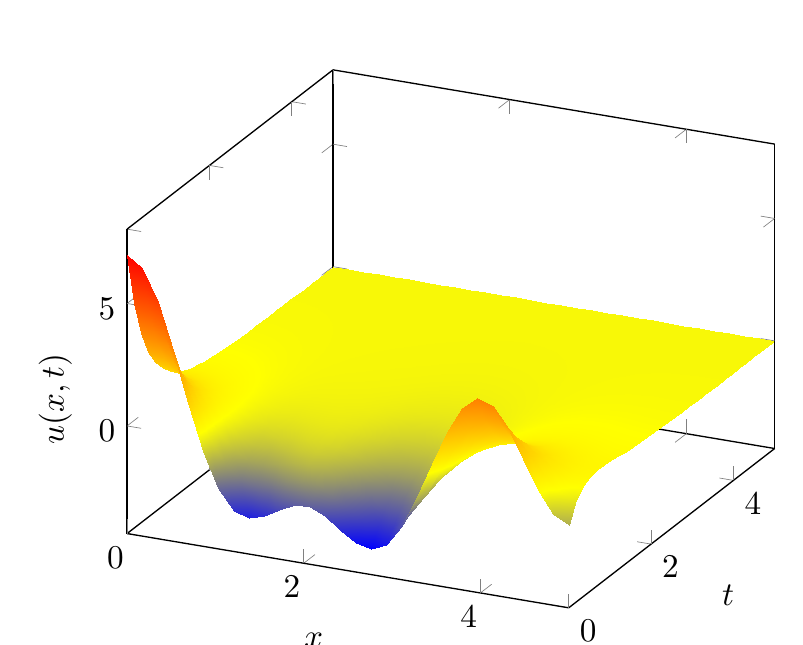
\begin{tikzpicture}[scale=1.2]
        \pgfdeclarelayer{pre main}
        \pgfsetlayers{pre main,main}

        \begin{axis}[        
        xlabel = $x$,
        ylabel = $t$,
        zlabel = {$u(x,t)$}]
        \addplot3[surf,
        samples=30,
        domain=0:5,y domain=0:5,
        z buffer=sort,
        shader=interp,
]
        {3*(cos(deg(2*pi*x/5))*e^(-(4 * pi^2 * y)/(25))) + 2*(cos(deg(3*pi*x/5))*e^(-(9 * pi^2 * y)/(25))) + 2*(cos(deg(pi*x))*e^(-(pi^2 * y)/(5)))};
        \end{axis}
    \end{tikzpicture}
    \caption{Primer spreminjanja stanja na palici s časom}
\end{figure}

Oglejmo si toplotno enačbo na premici $\R$ (delamo se, da je izolirana od preostalega prostora).
Naj bo $u(x, t)$ temperatura v točki $x$ ob času $t$.
Potem je toplotna enačba $u_t = D u_{xx}$, kjer je $D$ difuzijska konstanta.
Za rešitev te enačbe potrebujemo začetni pogoj $u(x, 0) = f(x)$,
torej je $f(x)$ začetna porazdelitev temperature vzdolž $\R$.
Naj bo $f \in L^1 (\R)$. Uporabimo Fourierovo transformiranko na funkcijo $x \mapsto u(x, t)$
in dobimo 
$$\F (u_t) = \int_{-\infty} ^\infty e^{-2\pi i \xi x} u_t (x, t)\, dx = \frac{\partial}{\partial t} \left(\int_{-\infty} ^\infty e^{-2\pi i \xi x} u (x, t)\, dx\right).$$
Na drugi strani enačbe pa s Fourierovo transformacijo imamo
$$\F (D u_{xx}) = D \F (u_{xx}) (\xi) = D (2 \pi i \xi)^2 \F (u) (\xi).$$
Če vpeljemo oznako $U(\xi, t) = \F (u) (\xi)$, dobimo diferencialno enačbo oblike
$$U_t (\xi, t) = - (2 \pi \xi)^2 D U(\xi, t),$$
katere splošna rešitev je oblike $A e^{kt}$.
Torej je $U(\xi, t) = A(\xi) e^{-4 \pi^2 D \xi^2 t}$
ter $U(\xi, 0) = A(\xi) = \hat{f} (\xi)$, zato  
$$U(\xi, t) = \hat{f} (\xi) e^{-4 \pi^2 D \xi^2 t}.$$
Ker je $\F (e^{-a x^2}) (\xi) = \sqrt{\frac{\pi}{a}} e^\frac{-\pi^2 \xi^2}{a}$,
je $\F \left(\frac{1}{\sqrt{4 \pi D t}} e^{-\frac{x^2}{4 D t}}\right) = e^{-4 \pi^2 D \xi^2 t}$.
Definiramo $\frac{1}{\sqrt{4 \pi D t}} e^{-\frac{x^2}{4 D t}} = K(x, t)$ kot Gaussovo jedro.
Potem je $U(\xi, t) =\F (f) (\xi)\cdot \F (K) (\xi)$ in od tod sledi $u(x, t) = f * K(\cdot, t)$.
Tako dobimo
\begin{align*}
    u(x, t) &= \int_{-\infty} ^\infty f(y) K(x - y, t)\, dy\\
    &= \frac{1}{\sqrt{4 \pi D t}} \int_{-\infty} ^\infty e^{-\frac{(x - y)^2}{4 Dt}} f(y)\, dy\\
    &= \frac{1}{\sqrt{\pi}} \int_{-\infty} ^\infty e^{-s^2} f(x - s\sqrt{4Dt})\, ds
\end{align*}

\begin{opomba}
    Ta integral je v splošnem definiran le za $t > 0$.
    Če je $f$ omejena in zvezna, integral hitro konvergira in velja $u \in C^\infty (\R_x \times (0, \infty)_t)$.
    Opazimo tudi, da velja $K_t = D K_{xx}$, torej Gaussovo jedro reši toplotno enačbo 
    in je naš rezultat za $u$ smiseln.
\end{opomba}

\begin{trditev}
    Naj bo $f$ zvezna in omejena na $\R$.
    Potem je $\lim_{t \downarrow 0} u(x, t) = f(x)$ enakomerno na končnih intervalih $\R$.
\end{trditev}

\begin{dokaz}
    Naj bo $\varepsilon > 0$.
    Poglejmo razliko 
    $$|u(x, t) - f(x)| = \frac{1}{\pi} \left| \int_{-\infty} ^\infty e^{-s^2} (f(x - s\sqrt{4Dt}) - f(x))\, ds \right|$$
    Ker je $f$ omejena oziroma $\|f\|_\infty \leq M$, obstaja tak $N > 0$, da je
    \begin{align*}
        \frac{1}{\pi} \int_{-\infty} ^{-N} e^{-s^2} |f(x - s\sqrt{4 Dt}) - f(x)|\, ds
        &+ \frac{1}{\pi} \int_{N} ^{\infty} e^{-s^2} |f(x - s\sqrt{4 Dt}) - f(x)|\, ds\\
        &\leq \frac{4 M}{\pi} \int_{N} ^\infty e^{-s^2}\, ds < \frac{\varepsilon}{2}.
    \end{align*}
    Ostane še integral $$\frac{1}{\pi} \int_{-N} ^{N} e^{-s^2} |f(x - s\sqrt{4 Dt}) - f(x)|\, ds.$$
    Na končnih intervalih je $f$ enakomerno zvezna in za $s \in [-N, N]$ je $|s \sqrt{4 D t} | \leq N \sqrt{4 D t}$.
    Ko je $t$ dovolj majhen ($t < t_0$ za nek $t_0$), velja $|f(x - s \sqrt{4 D t}) - f(x)| < \frac{\varepsilon}{2}$
    za vsak $x$ iz nekega danega končnega intervala $x \in [a, b]$.
    Torej za $0 < t < t_0$ velja $|u(x, t) - f(x) | < \varepsilon$ za vse $x \in [a, b]$.
\end{dokaz}

\begin{posledica}[Weierstrassov izrek]
    Naj bo $f \in C([a, b])$ in naj bo $\varepsilon > 0$.
    Potem obstaja polinom $p$, da je $\|f - p\|_{\infty} < \varepsilon$ na $[a, b]$.
\end{posledica}


\begin{dokaz}
    Funkcijo $f$ zvezno razširimo na $\R$ z vrednostmi $0$ zunaj intervala $[a - 1, b + 1]$
    kot smo naredili poprej.
    Vemo, da $u(x, t) = \frac{1}{\sqrt{4 \pi D t}} \int_{-\infty} ^\infty f(y) e^{-\frac{(x - y)^2}{4Dt}}\, dy$
    konvergira enakomerno proti $f$ na $[a, b]$, ko gre $t \downarrow 0$ (pri tem bi lahko izbrali $D = 1$).
    Označimo $A = a -1$ in $B = b + 1$. Ker je razširitev $f$ enaka 
    $0$ zunaj $[A, B]$, je $$u(x, t) = \frac{1}{\sqrt{4 \pi D t}} \int_{A} ^B f(y) e^{-\frac{(x - y)^2}{4Dt}}\, dy.$$
    Torej $x \in [a, b]$ in $y \in [A, B]$.
    Naj bo za dani $\varepsilon > 0$ dovolj majhen $t_0$, da je 
    $\| u(x, t_0) - f(x)\|_\infty < \frac{\varepsilon}{2}$ na $[a, b]$.
    Izraz ${-\frac{(x - y)^2}{4Dt_0}}$ teče po omejenem intervalu na $\R$,
    torej lahko $e^{{-\frac{(x - y)^2}{4Dt_0}}}$ poljubno dobro enakomerno aproksimiramo na tem intervalu s Taylorjevim 
    polinomom v ${-\frac{(x - y)^2}{4Dt_0}}$, in sicer kot $\sum_0 ^N \frac{1}{n!} \left(-\frac{(x -y)^2}{4Dt_0}\right)^n.$
    To pa je polinom v $x$.
\end{dokaz}



\end{document}